\documentclass[]{dukedissertation2023}

%\documentclass[economy,twoside,bind]{dukedissertation}
% Use the second for a single-spaced copy suitable for duplex printing
% and binding.

% Other useful options (there are more options documented in Chapter 2):
%  * draft -- don't actually include images, print a black bar on overful
%             hboxes
%  * MS    -- Format for a Master's Thesis.  No UMI abstract page, some 
%             textual changes to title page.  


% Useful packages for dissertation writing:
\usepackage[T1]{fontenc}
\usepackage{titlesec}
\usepackage{amsmath, amssymb, amsfonts, amsthm, stmaryrd}
\usepackage[scr=rsfs]{mathalpha}
\usepackage{bm}
\usepackage{graphicx}
\usepackage[backend=biber,natbib,style=apa,]{biblatex}
\usepackage[title,titletoc]{appendix}
\usepackage{apptools}
%\usepackage{mathptmx} % Uncomment this to use Times instead of Palatino
\usepackage{color}
% \usepackage{mathabx} %If using Times, comment this out
\usepackage{multirow}
\usepackage{setspace}

% \usepackage{mathpazo} % Comment this out if you want to use Times instead of Pallatino
\usepackage{indentfirst}
\usepackage{enumitem}
% \usepackage{xfrac}
\usepackage{mathtools}
\usepackage{caption}
\usepackage{subcaption}
\usepackage{tabularx}
\usepackage{booktabs}
\usepackage{siunitx}
%\usepackage{lscape}
% Use the pdflscape package if you want the page to rotate
\usepackage{pdflscape}
%\usepackage{longtable}
\usepackage{listings}
\usepackage{xcolor}
\usepackage{pgfplots}\pgfplotsset{compat=1.18}
%\usepackage{acronym}
%\usepackage{showframe}
\usepackage{makecell}
\usepackage[super]{nth}
\usepackage{xr}

\setlist[itemize]{noitemsep,nolistsep}
\setlist[enumerate]{noitemsep,nolistsep}
\sisetup{per-mode = symbol}
\sisetup{uncertainty-mode = separate}
\sisetup{
	output-open-uncertainty = [,
	output-close-uncertainty = ],
	uncertainty-separator = \,
}

%\usepackage{cite}  % If you include this, hyperlink cites will
                     % break.  It's nice to use this package if your bibstyle
							% sorts entries by order-of-use, rather than
							% alphabetically (as plain does).
							
%Theorem, Lemma, etc. environments
\newtheorem{theorem}{Theorem}%[section]
\newtheorem{lemma}[theorem]{Lemma}
\newtheorem{proposition}[theorem]{Proposition}
\newtheorem{corollary}[theorem]{Corollary}
\newtheorem{result}[theorem]{Result}

% Personal commands and abbreviations.
%Define and personal commands here

%Graphics Path to find your pictures
\graphicspath{{./Pictures/}{./Chapter1}} %Add multiple paths if there are images in multiple spots



%-----------------------------------------------------------------------------%
% PREAMBLE 
%-----------------------------------------------------------------------------%
\author{Peiyi Chen}
\title{[Your Title Here Even If It Is Very Very Very Very Very Very Long. Truly It Is A Miraculously Long Title For A Dissertation]}
\supervisor{Johann Guilleminot}
\department{Mechanical Engineering and Materials Science} % Appears as Department of \department
% Declare dissertation subject used on UMI abstract page.  List of
% categories: http://dissertations.umi.com/duke/subject_categories.html
%\subject{[Your Subject Here]}

\date{2023} % Anything but the year is ignored.

% Copyright text.  If undefined, default is 'All rights reserved'
% (Example sets the text to a hyperlinked Creative Commons Licence)
\copyrighttext{All rights reserved except the rights granted by the \href{http://creativecommons.org/licenses/by-nc/3.0/us/}{Creative Commons Attribution-Noncommercial Licence}}

% Committee Members other than supervisor.  No more than five beyond the
% supervisor allowed.Do not include titles (e.g. `Dr.')
\defensedate{November 20, 2023 (TBD)}
\member{John Dolbow}
\member{Cate Brinson}
\member{David Carlson}
% \member{[Committee Member 4]}
% \member{[Committee Member 5]}
%-----------------------------------------------------------------------------%

%-----------------------------------------------------------------------------%
% HYPERREF: plain black hypertext references for ref's and cite's.
%-----------------------------------------------------------------------------%
\usepackage[pdftex, pdfusetitle, plainpages=false, bookmarks, bookmarksnumbered, colorlinks, linkcolor=black, citecolor=black, filecolor=black, urlcolor=black,linktoc=none]{hyperref}
\usepackage[capitalise]{cleveref}
\creflabelformat{equation}{#2#1#3}
\makeatletter

\newcommand\getfontsizeofheading{The current font size is: \fontname\font \f@size pt}
% print given font size in point and in its "font size" (i.e. larger or smaller)
\newcommand\getfontsizeforfontsizeclass[1]{{\string #1 is printed as #1  \fontname\font \f@size pt\par}}
% print the entire string in the size of the fontsize (i.e. larger or smaller)
\newcommand\printfontsizeforfontsizeclass[1]{{#1 \string #1 is printed in  \fontname\font \f@size pt\par}}
\makeatother

%% macro from Peiyi

\newtheorem*{remark}{Remark}
\newtheorem{prop}{Proposition}

%% MACROS
\newcommand\bfa{\boldsymbol{a}}
\newcommand\bfb{\boldsymbol{b}}
\newcommand\bfc{\boldsymbol{c}}
\newcommand\bfd{\boldsymbol{d}}
\newcommand\bfe{\boldsymbol{e}}
\newcommand\bff{\boldsymbol{f}}
\newcommand\bfg{\boldsymbol{g}}
\newcommand\bfh{\boldsymbol{h}}
\newcommand\bfi{\boldsymbol{i}}
\newcommand\bfj{\boldsymbol{j}}
\newcommand\bfk{\boldsymbol{k}}
\newcommand\bfl{\boldsymbol{l}}
\newcommand\bfm{\boldsymbol{m}}
\newcommand\bfn{\boldsymbol{n}}
\newcommand\bfo{\boldsymbol{o}}
\newcommand\bfp{\boldsymbol{p}}
\newcommand\bfq{\boldsymbol{q}}
\newcommand\bfr{\boldsymbol{r}}
\newcommand\bfs{\boldsymbol{s}}
\newcommand\bft{\boldsymbol{t}}
\newcommand\bfu{\boldsymbol{u}}
\newcommand\bfv{\boldsymbol{v}}
\newcommand\bfw{\boldsymbol{w}}
\newcommand\bfx{\boldsymbol{x}}
\newcommand\bfy{\boldsymbol{y}}
\newcommand\bfz{\boldsymbol{z}}
%
\newcommand\bfA{\boldsymbol{A}}
\newcommand\bfB{\boldsymbol{B}}
\newcommand\bfC{\boldsymbol{C}}
\newcommand\bfD{\boldsymbol{D}}
\newcommand\bfE{\boldsymbol{E}}
\newcommand\bfF{\boldsymbol{F}}
\newcommand\bfG{\boldsymbol{G}}
\newcommand\bfH{\boldsymbol{H}}
\newcommand\bfI{\boldsymbol{I}}
\newcommand\bfJ{\boldsymbol{J}}
\newcommand\bfK{\boldsymbol{K}}
\newcommand\bfL{\boldsymbol{L}}
\newcommand\bfM{\boldsymbol{M}}
\newcommand\bfN{\boldsymbol{N}}
\newcommand\bfO{\boldsymbol{O}}
\newcommand\bfP{\boldsymbol{P}}
\newcommand\bfQ{\boldsymbol{Q}}
\newcommand\bfR{\boldsymbol{R}}
\newcommand\bfS{\boldsymbol{S}}
\newcommand\bfT{\boldsymbol{T}}
\newcommand\bfU{\boldsymbol{U}}
\newcommand\bfV{\boldsymbol{V}}
\newcommand\bfW{\boldsymbol{W}}
\newcommand\bfX{\boldsymbol{X}}
\newcommand\bfY{\boldsymbol{Y}}
\newcommand\bfZ{\boldsymbol{Z}}
%
\newcommand\bs[1]{\boldsymbol{#1}}

\newcommand{\defgrad}{\bfF}
\newcommand{\rcg}{\bfC}
\newcommand{\grad}{\boldsymbol{\nabla}}
\DeclareMathOperator{\tr}{tr}
% \newcommand\hmmax{0}
% \newcommand\bmmax{0}
%%
%%

\AtBeginBibliography{\vspace*{\baselineskip}}
\setlength{\bibitemsep}{\baselineskip}

%\titleformat{\chapter}
%	{\Large\bfseries\usefont{T1}{phv}{b}{n}\fontsize{16pt}{\baselineskip}} %Format
%	{\thechapter.} %Label
%	{\fontdimen2\font\space} %Sep
%	{\normalbaselines} % Before 

%\renewcommand{\thesection}{\arabic{chapter}.\arabic{section}}
%\renewcommand{\thesubsection}{\arabic{chapter}.\arabic{section}.\arabic{subsection}}
%\renewcommand{\thesubsubsection}{\arabic{chapter}.\arabic{section}.\arabic{subsection}.\arabic{subsubsection}}

\titleformat{\section}[block]{\fontencoding{T1}\fontfamily{phv}\fontseries{b}%
  \fontshape{it}\fontsize{14pt}{11}\selectfont}{\thesection}{.2em}{\normalbaselines}
 \titleformat{\subsection}[block]{\fontencoding{T1}\fontfamily{phv}\fontseries{b}%
  \fontshape{n}\fontsize{13pt}{11}\selectfont}{\thesubsection}{.2em}{\normalbaselines}
 \titleformat{\subsubsection}[block]{\fontencoding{T1}\fontfamily{ppl}\fontseries{b}%
  \fontshape{n}\fontsize{11pt}{11}\selectfont}{\thesubsubsection}{.2em}{\normalbaselines}
  
  
\titlespacing\section{0pt}{14pt plus 0pt minus 0pt}{6pt plus 0pt minus 0pt}
\titlespacing\subsection{0pt}{14pt plus 0pt minus 0pt}{6pt plus 0pt minus 0pt}
\titlespacing\subsubsection{0pt}{14pt plus 0pt minus 0pt}{6pt plus 0pt minus 0pt}
\titlespacing\paragraph{0pt}{6pt plus 0pt minus 0pt}{6pt plus 0pt minus 0pt}
\titlespacing\subparagraph{0pt}{6pt plus 0pt minus 0pt}{6pt plus 0pt minus 0pt}

\setcounter{secnumdepth}{4}

\newcolumntype{L}[1]{>{\raggedright\let\newline\\\arraybackslash\hspace{0pt}}b{#1}}
\newcolumntype{C}[1]{>{\centering\let\newline\\\arraybackslash\hspace{0pt}}b{#1}}
\newcolumntype{R}[1]{>{\raggedleft\let\newline\\\arraybackslash\hspace{0pt}}b{#1}}

\usepackage{subfiles}
\addbibresource{./Bibliography/mybib.bib} %your bibliography file - change the path if needed
\begin{document}

%-----------------------------------------------------------------------------%
% TITLE PAGE -- provides UMI abstract title page & copyright if appropriate
%-----------------------------------------------------------------------------%
\maketitle

%-----------------------------------------------------------------------------%
% ABSTRACT -- included file should start with '\abstract'.
%-----------------------------------------------------------------------------%
\abstract
In the abstract, you must (1) present the problem of the thesis/dissertation, (2) discuss the materials and methods used, and (3) state the conclusions reached. Individual chapters should not have abstracts.
 
Note that this will be the first numbered page: it is page \textit{iv}; pages \textit{i}, \textit{ii} and \textit{iii} (copyright, signature page and abstract signature page) were counted but not numbered. If you look ahead, you will see that numbering up to the first page of text is in roman numerals. On the first page of Introduction or Chapter One, begin numbering at Arabic number 1. This numbering (1, 2, 3, 4 \dots) is consecutive through the rest of the document. 

Also note that the page margins are set with a 1.5-inch margin on the left side and a 1-inch margin on the top, right side, and bottom, throughout the entire document.

The page number below should be above the 1-inch margin and centered to the page margins, not the page edges.

%-----------------------------------------------------------------------------%
% DEDICATION -- OPTIONAL.  Put the text inside the braces.
%               (Long 'dedications' probably belong in the acknowledgements)
%-----------------------------------------------------------------------------%
% \dedication{If you want to dedicate your thesis to anyone do so here.}

%-----------------------------------------------------------------------------%
% FRONTMATTER -- ToC is required, LoT and LoF are required if you have any
% tables or figures, respectively. List of Abbreviations and Symbols is 
% optional.
%-----------------------------------------------------------------------------%
\tableofcontents % Automatically generated

\listoftables	% If you have any tables, automatically generated

\listoffigures	% If you have any figures, automatically generated

%\include{./Abbreviations/listofabbr} % List of Abbreviations. Start file with '\abbreviations'

%-----------------------------------------------------------------------------%
% ACKNOWLEDGEMENTS -- included file should start with '\acknowledgements'
%-----------------------------------------------------------------------------%
\acknowledgements

I would like to deeply thank my PhD advisor, Professor Johann Guilleminot, for the wealth of knowledge I have acquired under his guidancethe, and the amazing time that we worked together. He is a wonderful mentor and dedicated coolaborator, and always an inovative researcher. In moments of challenge throughout my doctoral journey, he consistently offers invaluable insights during discussions and provides assistance in resolving issues. His devotion and passion to his research inspired and motivated me to become a committed and serious engineer.

I would like to extend my gratitude to my esteemed collaborator, Professor Christian Soize, whose significant contributions have played a crucial role in bringing this dissertation to completion. I would also like to thank Professor John Dolbow, Professor Wilkins Aquino, Professor Hossein Salahshoor for accepting to evaluate this work.

I acknowledge the financial support of the Graduate School at Duke University. This work was partially funded by the National Science Foundation (NSF) under grants CMMI-1726403, CMMI-1942928, and DGE-2022040.

Last but not least, I thank my fiancé Gary, and my dog Rudy for believing in me and supporting me during all these years.

%==============================================================================
%-----------------------------------------------------------------------------%
%
% MAIN BODY OF PAPER
%
%
%-----------------------------------------------------------------------------%
\chapter{Introduction}
\label{chap:Introduction}

The mathematically-consistent representation and identification of parametric uncertainties is a central task of uncertainty quantification (UQ) in computational mechanics. From a mechanics of materials standpoint \cite{GUILLEMINOT2020385}, such fluctuations can be primarily attributed to subscale variability, which itself---and most often---stems from complex processing conditions for engineered composites (such as fiber-reinforced composites or concrete), or evolution-based optimization in the case of biological tissues. There has been a tremendous amount of works focusing on the integration of such uncertainties in the past three decades. Labeled statistical distributions, such as Gaussian, Gamma, and lognormal distributions, are generally assumed to model homogeneous stochastic inputs. The choice of these distributions is sometimes arbitrarily made or based on data fitting (which may lead to ill-posed forward problems), and can facilitate uncertainty propagation through spectral approaches \cite{Ghanem1991, OLM, Ghanem2017} where quantities of interest are represented by polynomial chaos surrogate models \cite{Wiener,Cameron,Xiu2002,Soize2004}. When an accurate microstructural description is not possible, due to data limitation, prior models can be constructed that capture available physical information, such as anisotropy, as well as mathematical constraints related to well-posedness for the associated forward propagation problem. Information-theoretic contributions proceeding along those lines can be found in \cite{Soize2006,Guilleminot-IJNME-2017,Guilleminot-SIAM-2013,STABER2017399} for the case of tensor-valued coefficients in linear differential operators, to list a few; see also \cite{Grigoriu2016} for yet another type of methodology, as well as \cite{SOIZE2011} for integration within a Bayesian setting.

While traditional approaches have established a solid foundation for uncertainty quantification in computational mechanics, the complex nature of certain materials demands more adaptive and data-driven approaches. Lately, constitutive models based on neural networks (NN) have also received growing attention over the past few years, owing to their ability to represent nonlinear mappings in a high dimensional setting. There is a very substantial amount of papers published on this topic, for a wide variety of material behaviors; see, \textit{e.g.},  \cite{flaschel2021unsupervised,xu2021learning,holzapfel2021predictive,jung2006neural,ghaboussi1998autoprogressive,ghaboussi1998new,hashash2004numerical,furukawa1998implicit,joshi2022bayesian,as2022mechanics,Asad-IJNME,KLEIN2022104703} and the references therein, in a non-exhaustive manner. Beyond classical data science aspects that pertain to architecture design, training and validation strategies, and the analysis of approximation capabilities, a central concern is to make such surrogates amenable to scientific simulations where such models are typically set to parameterize systems of partial differential equations. In this context, the surrogate must satisfy both physical assumptions and mathematical properties (\textit{e.g.}, boundedness or a certain type of convexity) to ensure the existence (and potentially, the uniqueness) of solutions. From the interests of mathematically-consistent representations, where precision and robustness are significant, we know that a high-fidelity simulation, oftentimes in the form of coupled partial differential equations (PDEs), is computationally prohibitive as a feasible forward simulation within the outer loop in many decision-making applications, e.g. inverse problem, optimal control, uncertainty quantification, etc. To avoid evaluating the expensive high-fidelity model in a forward simulation, a reduced order model (ROM) can be trained as its surrogate with reasonable accuracy, hence significantly reducing the computational cost allowing for faster simulations and real-time applications without sacrificing the essence of the underlying mathematical principles. Nonlinear PDEs describe a wide spectrum of engineering problems. High-fidelity numerical solvers based on high-dimensional spatial discretizations are prohibitively expensive in many-query settings. Intrusive and non-intrusive LS-ROMs reduce the dimensionality of the model by projecting the solution of the high-dimensional model onto a linear subspace. Several approaches to defining the approximation subspace have been proposed (see e.g. \cite{benner2015survey} for a review). A common empirical choice is the proper orthogonal decomposition (POD) subspace, which spans the leading principal components of an available set of state data \cite{berkooz1993proper,lumley1967structure,sirovich1987turbulence}. For PDEs with only linear and polynomial terms, the projection-based reduced model admits an efficient low-dimensional numerical representation that can be cheaply evaluated at a cost independent of the dimension of the original model \cite{benner2015two,benner2015survey,cuong2005certified,goyal2016algebraic,hesthaven2016certified}. For PDEs with more general nonlinear terms, an additional level of approximation, e.g., interpolation \cite{astrid2008missing,barrault2004empirical,carlberg2013gnat,chaturantabut2010nonlinear,drmac2016new,grepl2007efficient,nguyen2008best}, is generally needed to achieve computational efficiency. Alternatively, the works in \cite{benner2015two,goyal2016algebraic,kramer2019nonlinear,kramer2019balanced} transform PDEs with general nonlinear terms to representations with only quadratic nonlinearities via the use of structure-exposing lifting transformations, and then project the quadratic operators of the resultant lifted PDE to obtain a reduced model. In recent years, machine learning based approaches to NM-ROMs have received an increasing interest. Some treat the weights and biases of a deep neural network (DNN) as unknowns in the solution process \cite{dissanayake1994neural,lagaris1998artificial,meade1994numerical,van1995neural}, while others incorporate physical laws into DNN-based surrogates whose weights and biases are determined in the training phase \cite{han2018solving,lu2019deeponet,lu2021deepxde,pang2019fpinns,raissi2019physics,lee2020model,lee2019deep}. 

Notet that uncertainties within nonlinear constitutive models can be defined in a multiscale framework where material parameters are made random. Concurrent nonlinear simulations involve the strong coupling between a macroscopic (or structural) formulation and a microscopic description capturing subscale details \cite{ghosh1996two,smit1998prediction,feyel1999multiscale,feyel2000fe2,terada2001class,kouznetsova2002multi,geers2016multiscale,raju2021review}. One popular approach is the so-called FE$^2$ method \cite{feyel1999multiscale,feyel2000fe2}, where information (in the form of a deformation gradient and any adapted stress variable) is transferred back-and-forth between quadrature points at the macroscale and statistical or representative volume elements (depending on whether the separation of scales exists or not). While versatile and powerful, such frameworks require significant computational resources that often surpass the capabilities of intermediate-power computers, especially when the underlying behavior is highly nonlinear. In this context, the development of surrogate models for large-scale systems has become a very active research domain and has generated a substantial body of literature. Various methodologies have been proposed to address this challenge, including (in a non-exhaustive manner) the development of deterministic representations \cite{yvonnet2007reduced,monteiro2008computational,yvonnet2009numerically, temizer2007adaptive,temizer2007numerical,fritzen2013reduced,bhattacharjee2016nonlinear, yvonnet2013computational,fritzen2018two,liu2016self,han2020efficient,feng2021concurrent} and probabilistic/statistical-based approaches \cite{efendiev2004multiscale,efendiev2009multiscale,weinan2003heterognous,weinan2007heterogeneous,abdulle2013adaptive,abdulle2012heterogeneous}, and more recently, the integration of machine learning (ML) tools, both with and without probabilistic/statistical formulations; see, e.g., \cite{le2015computational,rao2020three,lu2019data,leung2022nh,nguyen2019surrogate,minh2020surrogate,feng2022finite,han2023neural,wessels2022computational,black2023deep}. In most of the above contributions, the multiscale surrogate is built either through polynomial approximations or deep learning models, and applied \textit{locally} at each point of the coarse scale discretization. In these settings, the intrinsic randomness --- and potential non-locality --- induced by random media with non-separated scales is very challenging to capture due to representation limitations.

The goal of this thesis lies in the construction of mathematically-consistent representation for deep learning methods and uncertainty quatification in computational mechanics. We consider the class of hyperelastic models with a specific interest in soft biological tissues characterized by extensive variability attributed to factors like age, gender, health conditions and microstructural complexity. Uncertainties raised by these factors make it chanllenging to applications such as computer-assisted diagnostics and surgical procedures or the growth of compatible artificial substitutes.

\section{Research Contributions}

\begin{itemize}
    \item[1.] We develop a stochastic model for the spatially-dependent material parameters parameterizing anisotropic strain energy density functions. The construction is cast within the framework of information theory, which is invoked to derive a least-informative model while ensuring consistency with theoretical requirements in finite elasticity. Specifically, almost sure polyconvexity and uniform growth conditions are enforced through proper repulsion constraints and regularization, hence making the forward problem of uncertainty propagation well posed. In addition, transformations arising from the linearization procedure are introduced for consistency and induce statistical dependencies in the primary variables. The latter include material moduli, a weight balancing between the isotropic and anisotropic contributions, and the angle defining the structural tensors. The identification of the model is subsequently performed, using an existing database on human arterial walls. Maximum likelihood estimators are obtained and provided for the adventitia, media, and intima layers, which enables the use of the proposed model as a generative surrogate for, e.g., training and classification in data-driven approaches integrating inter-patient variability. Finally, uncertainty propagation on a realistic, patient-specific geometry is conducted to demonstrate the efficiency of the stochastic modeling framework.
    \item[2.] We propose a simple approach to rectify unconstrained neural networks for hyperelastic constitutive models with the aim of ensuring both mathematical well-posedness (in terms of existence theorems) and physical consistency. The surrogate involves neural networks that are made admissible by selecting a proper parameterization, following standard results in continuum mechanics, and by enforcing polyconvexity through integral representations. We also demonstrate the relevance of the formulation by considering digitally synthesized and experimental datasets for isotropic and anisotropic materials, including the case of soft biological tissues.
    \item[3.] We develop a nonlinear manifold reduced order model (NM-ROM) based on Convolutional Neural Network-based autoencoders (CNNAE) with iteration-dependent trainable kernels inspired from adpative basis methods. We investigate DNN-based operator inference strategies between latent spaces, and propose a strategy to perform vectorized implicit time integration. We demonstrate that the proposed CNN-based NM-ROM, combined with DNN-based operator inference, generally performs better than commonly employed strategies (in terms of prediction accuracy) on a benchmark advection-dominated problem. The method also presents substantial gain in terms of training speed per epoch, with a training time about one order of magnitude smaller than the one associated with a state-of-the-art technique performing with the same level of accuracy.
    \item[4.] We present a methodology that addresses the construction of statistical surrogates for concurrent multiscale modeling in structures comprising nonlinear random materials from the point of view of probabilistic learning. More specifically, we formulate the approximation problem using conditional statistics, and use probabilistic learning on manifolds to draw samples of the nonlinear constitutive model at mesoscale accelerating multiscale computations bypass solving the nonlinear boundary problems at the mesocopic scale. Two applications, relevant to inverse problem solving and forward propagation, are presented in the context of nonlinear elasticity. The framework enables accurate predictions (in probability law), despite the small amount of training data and the very high levels of nonlinearity and stochasticity in the considered system.
\end{itemize}

\section{Organization of the dissertation}

In Chapter~\ref{chap:artery}, we revisit and extend the methodological steps presented in \cite{STABER201894} to model spatially-varying stochastic anisotropic strain energy density functions. The regularization is imposed on the isotropic part of the strain energy density function and the parameterization is extended to account for fluctuations and waviness in the structural tensors and covariance kernel. We also address the identification of the model based on experimental results available on human arterial walls, with the goal of providing interested readers with the capability to generate datasets that are consistent with inter-patient fluctuations. In Chapter~\ref{chap:polyconvex}, we construct a convex neural network model without affecting expressiveness (that is, without constraining weights \textit{a priori}) and training cost (which can be affected by transformations performed on weights at the training stage). The rectified neural network models is then deployed on digitally synthesized and experimental datasets, relevant to both isotropic and anisotropic materials. In Chapter~\ref{chap:cnnae}, we devise a novel structure for the decoder in the NM-ROM, such that the underlying nonlinear mapping closely resembles the formulation of adaptive basis methods. We also propose a DNN-based reduced operator inference that learns from the latent space for full models based on time-dependent partial differential equations. In Chapter~\ref{chap:fe2}, we introduce a statistical surrogate model for concurrent multiscale simulations involving nonlinear materials with non-separated scales. The methodology combines probabilistic learning on manifolds, a generative model that allows for measure concentration and support information to be accurately captured, with the use of conditional statistics to approximate the mapping between apparent strain and stress variables --- namely, the right Cauchy-Green tensor and the second Piola-Kirchhoff stress tensor --- at a finite set of points (defining a subregion of interest where concurrent coupling must be deployed). In the Section~\ref{sec:intro-background}, we'll briefly recall the framework of continuum mechanics of hyperelastic materials that will be used in this work.

\section{Notation}

\noindent (i) {\textit{Conventions for variables}}.\\
A lower-case Latin or Greek letter, such as $x$ or $\eta$, is a deterministic real variable.\\
A boldface lower-case Latin or Greek letter, such as $\bfx$ or $\bfeta$, is a deterministic vector.\\
An upper-case Latin or Greek letter, such as $X$ or $\Xi$, is a real-valued random variable.\\
A boldface upper-case Latin letter, such as $\bfX$, is a vector-valued random variable.\\
A lower- or upper-case Latin letter between brackets, such as $[x]$ or $[X]$, is a deterministic matrix.\\
A boldface upper-case letter between brackets, such as $[\bfX]$, is a matrix-valued random variable.\\

\noindent (ii) {\textit{Probability space, random variable, probability measure, and probability density function.}}\\
For any finite integer $m\geq 1$, the Euclidean space $\RR^m$ is equipped with the $\sigma$-algebra $\curB_{\RR^m}$.
If $\bfY$ is a $\RR^m$-valued random variable defined on the probability space $(\Theta,\curT,\curP)$, $\bfY$ is a  mapping $\theta\mapsto\bfY(\theta)$ from $\Theta$ into $\RR^m$, measurable from $(\Theta,\curT)$ into $(\RR^m,\curB_{\RR^m})$,
and $\bfY(\theta)$ is a realization (sample) of $\bfY$ for $\theta\in\Theta$. 
The probability distribution of $\bfY$ is the probability measure $P_{\bfY}(d\bfy)$ on the measurable set $(\RR^m,\curB_{\RR^m})$ (we will simply say on $\RR^m$). 
The Lebesgue measure on $\RR^m$ is denoted by $d\bfy$ and $P_{\bfY}(d\bfy) = p_{\bfY}(\bfy)\, d\bfy$, with $p_{\bfY}$ the probability density function (pdf) on $\RR^m$ of $P_{\bfY}(d\bfy)$ with respect to $d\bfy$.
Finally, $E$ denotes the mathematical expectation operator.\\

\noindent (iii) {\textit{Algebraic notations}}.\\
$\RR$: set of all the real numbers.\\
$\RR^n$: Euclidean vector space on $\RR$ of dimension $n$.\\
$\MM_{n,m}$: set of all the $(n\times m)$ real matrices.\\
$\MM_n$: set of all the square $(n\times n)$ real matrices.\\
$\MM_n^+$: set of all the positive-definite symmetric $(n\times n)$ real matrices.\\
$[I_{n}]$: identity matrix in $\MM_n$.\\
$\bfx = (x_1,\ldots,x_n)$: point in $\RR^n$.\\
$\langle \bfx,\bfy \rangle = x_1 y_1 + \ldots + x_n y_n$: inner product in $\RR^n$.\\
$\Vert\,\bfx\,\Vert$:  norm in $\RR^n$ such that $\Vert\,\bfx\,\Vert = \langle \bfx,\bfx \rangle$.\\
$[x]^T$: transpose of matrix $[x]$.\\
$\Vert\, [x]\, \Vert$: Frobenius norm of matrix  $[x]$.\\
$\delta_{kk'}$: Kronecker's symbol.

\section{Background}
\label{sec:intro-background}
\subsection{Constitutive Modeling for Arterial Tissues}
\label{subsubsec:constitutive-modeling}
Let $B$ be a collection of material points identified with their vector of coordinates $\bfx$ in $\mathbb{R}^3$, and denote by $\partial B$ the boundary of $B$. For any material point $\bfx \in B$, the spatial point $\bfx_\varphi$ in the deformed configuration $B_\varphi$ is given by $\bfx_\varphi = \varphi (\bfx)$, where $\varphi$ is the deformation map. For any $\bfx \in B$, the deformation gradient $\bfF$ is a second-order tensor defined as $\bfF = \boldsymbol{\nabla}_{\bfx} \bfx_\varphi$. The right Cauchy-Green deformation tensor is defined as $\bfC = \bfF^T \bfF$. For later use, we introduce the isochoric counterpart $\overline{\bfC}$ of $\bfC$, defined as $\overline{\bfC} = J^{-2/3}\bfC$, with $J = \det(\bfF)$ the Jacobian of the transformation. Notice that notations $\bfx$ and $\bfx_\varphi$ to denote points in the reference and deformed configurations, respectively, is unusual in the literature of finite elasticity \cite{Ciarlet1988} but is introduced for the sake of consistency with the rest of this paper---where deterministic vector-valued variables are represented with bold lowercase symbols.

Following standard assumptions \cite{Holzapfel2000,Gasser2006,Holzapfel2010,Holzapfel2015,Holzapfel2017} (see also \cite{Brinkhues2013ModelingAS} and the references therein for instance), the material is assumed to be hyperelastic, nearly-incompressible, and anisotropic. Note that while a transversely isotropic model is considered hereinafter, due to the considered application, the methodological ingredients related to the construction of the stochastic model remain valid for other classes of anisotropy. The nonlinear constitutive model is thus defined by a strain energy density function $\psi:\mathbb{M}^3_+ \to \mathbb{R}$ taken as
\begin{align}
    \psi(\bfF) = \psi^{\text{MR}}(\bfF) + \psi^\text{p}(\bfF) + \sum_{k=1}^{2} \psi_{(k)}^\text{ti}(\bfF)\,, \label{eq: strain energy density function}
\end{align}
in which $\psi^{\text{MR}}$ denotes an isochoric Mooney-Rivlin strain energy density function, $\psi^\text{p}$ is a penalty term used to account for the near-incompressibility constraint \cite{charrier1988existence}, and $\{\psi_{(k)}^\text{ti}\}_{k = 1}^2$ are anisotropic strain energy density functions to be defined momentarily. The Mooney-Rivlin contribution is given by
\begin{align}
    \psi^{\text{MR}}(\bfF) &= \mu_1 \left( \textnormal{tr}(\overline{\bfC}) - 3 \right) + \mu_2 \left( \textnormal{tr}(\text{Cof}(\overline{\bfC}))^{3/2} - 3^{3/2}\right) \label{eq: MR} 
\end{align}
with a slight abuse of notation, where $\mu_1$ and $\mu_2$ are strictly positive material parameters, ``$\textnormal{tr}$'' denotes the trace operator and ``$\text{Cof}$'' is the matrix of cofactors, $\text{Cof}(\overline{\bfA}) = \det(\bfA)\bfA^{-T}$ for any matrix $\bfA$. The penalty term is given by
\begin{align}
    \psi^\text{p}(\bfF) & = \mu_3 (J^{\beta_3}+J^{-\beta_3} - 2)\,, \label{eq: penalty}
\end{align}
where $\mu_3 \in \mathbb{R}_{> 0}$ and $\beta_3 \in \mathbb{R}_{> 2}$ are viewed as numerical model parameters. The anisotropic contribution modeling the stiffening effect of the tissue in tension (only), along a direction defined by a unit vector $\bfa^{(k)}$, is defined as
\begin{equation}
    \psi_{(k)}^\text{ti}(\bfF) = \frac{\mu_4}{\beta_4} \left\{ \exp \left(\beta_4 \left( (1-\rho)(\textnormal{tr}(\bfC)-3)^2 + \rho (\vert \vert \bfF \bfa^{(k)} \vert \vert ^2_2 - 1)^2 \right) \right) - 1\right\}\,, \label{eq: psi tissue-artery}
\end{equation}
where $\mu_4 \in \mathbb{R}_{> 0}$, $\beta_4 \in \mathbb{R}_{> 0}$, and $\rho \in [0,1]$ are material parameters \cite{holzapfel2005determination}. Following standard modeling assumptions, the unit vectors $\bfa^{(1)}$ and $\bfa^{(2)}$ are defined as
\begin{equation}    
    \bfa^{(1)} = \cos(\alpha) \bfe^{(1)} + \sin(\alpha)\bfe^{(2)}\,, \quad 
    \bfa^{(2)} = \cos(\alpha) \bfe^{(1)} - \sin(\alpha)\bfe^{(2)}\,,
\end{equation}
where $\bfe^{(1)}$ and $\bfe^{(2)}$ are unit vectors defining a local basis at every location $\bfx$ in the reference configuration, and $\alpha$ is the angle between tissue orientation and the aforementioned basis. Notice that $\psi_{(1)}^\text{ti} = \psi_{(2)}^\text{ti}$ in this case, owing to the evenness of the right-hand side in Eq.~\eqref{eq: psi tissue-artery}.

\begin{prop}
The stored energy density function $\psi$ defined by Eq.~\eqref{eq: strain energy density function} is polyconvex and satisfies proper growth conditions, hence ensuring the well-posedness of the nonlinear boundary value problem \cite{Ciarlet1988,ball2002some}.
\end{prop}

\begin{proof} 
The strain energy density function $\bfF \mapsto \psi(\bfF)$ is polyconvex if and only if there exists a convex function $\psi^*$ such that
\begin{align}
    \psi(\bfF) & = \psi^*(\bfF, \text{Cof}(\bfF), \det(\bfF))
\end{align}
for all $\bfF$ in $\mathbb{M}^3$. For an additive decomposition, the above requirement amounts to showing that each term in $\psi$ is a convex function in the associated variable. For the isotropic contribution, the convexity of the functions $\bfF \mapsto \textnormal{tr}(\overline{\bfC}) = \vert \vert \bfF \vert \vert_F^2/(\det(\bfF))^{2/3}$ and $\bfF \mapsto \textnormal{tr}(\text{Cof}(\overline{\bfC}))^{3/2} = \vert \vert \text{Cof}(\bfF) \vert \vert_F^3/(\det(\bfF))^2$ was established in many references; see, e.g., \cite{hartmann2003polyconvexity,schroder2003invariant}. Regarding the anisotropic counterpart, notice first that the convexity of the function $\bfF \mapsto \langle \vert \vert \bfF \bfa_k \vert \vert ^2-1 \rangle^2_m$ was shown in \cite{balzani2006polyconvex}. Since the function $\bfF \mapsto \textnormal{tr}(\bfC)$ is convex, it then follows that the convex combination $(1-\rho)(\textnormal{tr}(\bfC)-3)^2 + \rho \langle \vert \vert \bfF \bfa_k \vert \vert ^2-1 \rangle^2_m$, with $\rho \geq 0$,  also defines a convex function in $\bfF$. For $\beta_4 > 0$, the exponential term in Eq.~\eqref{eq: psi tissue-artery} is thus the composition of a (strictly) convex nondecreasing function and a convex function, and is therefore convex. For $\mu_4 > 0$, the strain energy density function defined is hence polyconvex. For growth conditions, see, e.g., \cite{ball2002some}.
\end{proof}

\subsection{Definition of the Boundary Value Problem}\label{subsec:def-NBVP}

In a general setting, the strong form of the boundary value problem (balance of linear momentum) in the reference configuration is stated as \cite{wriggers2008nonlinear}
\begin{align}
    \boldsymbol{\nabla}_{\bfx} \bf{P} + \bf{b}  = {\bf{0}}\,,& \quad \forall\,\bfx \in {B}\,, \label{eq: stress divergence}\\
    \bfu = \overline{\bfu}\,,& \quad \forall\, \bfx \in \partial B_D\,,\\
    \bfP \cdot \bfN = \overline{\bft}\,,& \quad \forall\, \bfx \in \partial B_N\,,
\end{align}
where $\boldsymbol{\nabla}_{\bfx}$ denotes the divergence operator in the reference configuration, $\bfP$ is the first Piola-Kirchhoff stress tensor defined as
\begin{equation}
    \bfP = \displaystyle{\frac{\partial w(\bfF)}{\partial \bfF}}\,,
\end{equation}
the vector $\bfb$ is the body force, $\bfN$ is unit vector normal to the boundary in the reference configuration, $\overline{\bfu}$ and $\overline{\bft}$ are given smooth vector fields on the Dirichlet and Neumann boundaries, denoted by $\partial B_D$ and $\partial B_N$ respectively. The solution to the above problem is classically sought (in an appropriate function space) as a stationary point of the following energy functional \cite{wriggers2008nonlinear}:
\begin{align}
    \Pi(\varphi) &= \int_B \psi(\bfF) \, dV - \int_{B} \bfb \cdot \varphi\,dV - \int_{\partial B_N} \overline{\bft} \cdot \varphi\,dA\,.
\end{align}
\chapter{Spatially-Dependent Material Uncertainties in Anisotropic Nonlinear Elasticity: Stochastic Modeling, Identification, and Propagation}
\label{chap:artery}

An underlying Gaussian measure, usually reduced by means of a Karhunen-Lo\`{e}ve expansion (to tackle the so-called curse of dimensionality) and pushed-forward by a given (e.g., exponential) transformation (to ensure almost sure positiveness as coefficient in an elliptic operator for instance), is usually invoked for heterogeneous inputs, described as random fields \cite{Ghanem1991,Ghanem2017}. Alternatively, input probability measures for constitutive models may be \textit{implicitly} described through scale-bridging procedures where microstructural features are modeled \cite{Sobczyk,Torquato}, homogenized at mesoscale \cite{OstojaBook, ostoja1998, baxter2001a, baxter2001b, STEFANOU2017319}, and potentially integrated within generic frameworks for dimensionality reduction \cite{BESSA2017633} and materials design \cite{Yin2009}. Such approaches can provide more realistic descriptions of material variability, owing to the fact that they rely on a mechanistic, multiscale-informed generator for the stochastic inputs.

Modeling contributions in the context of nonlinear behavior are far more scarce. As with the case of linear elasticity, implicit descriptions can be obtained through computational homogenization; see \cite{Clement2012,Clement2013} for hyperelastic microstructures, and \cite{OZTURK2021104294} for plasticity. Another approach aimed at prescribing dependencies evaluated through the statistical treatment of a digital database on hyperelastic solids was reported in \cite{caylak2018stochastic}. The first attempts to construct stochastic models for hyperelastic materials based on information theory can be found in \cite{staber2015stochastic} and \cite{Staber2017zamm} for the incompressible and compressible (homogeneous) cases, respectively. Here, constraints related to polyconvexity and linearization at small strains were considered to ensure well-posedness and introduce statistical dependencies between the primary material parameters. Such models were used to identify the probabilistic behavior of soft biological tissues based on physical experiments in \cite{STABER2017743}, and to investigate a series of theoretical propagation problems in \cite{Mihai-1, Mihai-2, Mihai-3, Mihai-4} (see also \cite{mihai2018stochastic}). These developments served as the basis to address the heterogeneous case, where properties are allowed to vary spatially, in \cite{STABER201894}. In addition to admissibility, the model also enforced the structural compliance of the covariance kernel on patient-specific geometries by relying on noise filtering---a technique that we will use in this paper as well. The methodology was later used in \cite{staber2019stochastic} to identify fluctuations in the anisotropic strain energy density function defining a composite laminate. Finally, a Bayesian approach relying on a regular covariance kernel (evaluated with the Euclidean metric) was proposed in \cite{Biehler2015}; see also \cite{fitt2019uncertainty} for Bayesian model selection for the homogeneous case. 

We restrict the analysis to the passive mechanical response of the artery: the integration of the active component, which can play an important role in vivo \cite{YOSIBASH201251}, is left for future study. To the authors' best knowledge, this represents the first contribution where both the stochastic model and the calibrated hyperparameters are presented in a self-contained manner. This may, in particular, support the development of data-driven frameworks, which are increasingly used to model and classify the behavior of such soft biological tissues (see \cite{Holzapfel2021} as an example). It is also important to note that the methodology of construction is applicable for modeling other classes of materials, such as engineered composite laminates that can be experimentally characterized through full-field measurement techniques.

This section is structured as follows. In Section~\ref{sec:background-det-nonlin}, we recall the necessary background pertaining to constitutive modeling in finite elasticity. In Section~\ref{sec:sto-homogeneous}, we address the modeling of stochastic stored energy functions parameterized by homogeneous random coefficients. These results are subsequently invoked and extended in Section \ref{sec:sto-heterogeneous} where we consider the case of spatially-dependent material parameters, modeled as non-Gaussian random fields. Calibration aspects are discussed in Section \ref{sec:calibration}, using physical experiments taken from the literature. Uncertainty propagation on patient-specific geometries is finally conducted in Section \ref{sec:uncertainty-propagation}.

\section{Background in Nonlinear Elasticity}
\label{sec:background-det-nonlin}


\subsection{Elasticity Tensor at Small Strains} \label{Linearization}
We conclude this section by deriving the linearized elasticity tensor at small strains associated with the deterministic strain energy density function $\psi$. This calculation will be used, in Section \ref{sec:sto-homogeneous}, to introduce suitable constraints, as well as an ad hoc parameterization, in the stochastic models. The small strain elasticity tensor is denoted by $\mathbb{C}$ and is defined as (see \cite{Holzapfel-Book-2000} for instance)
\begin{equation}
    \mathbb{C} = \left.4\frac{\partial^2 \psi}{\partial \bfC \partial \bfC}\right\vert_{\bfC = \bfI}\,. \label{eq:elasticity-def}
\end{equation}
Following Eq.~\ref{eq: strain energy density function}, we introduce the decomposition
\begin{equation}
    \mathbb{C} = \mathbb{C}^{MR} + \mathbb{C}^{p} + \mathbb{C}^{ti}
\end{equation}
with
\begin{equation}
    \mathbb{C}^{\text{MR}} = \left.4\frac{\partial^2 \psi^{\text{MR}}}{\partial \bfC \partial \bfC}\right\vert_{\bfC = \bfI}\,, \quad
    \mathbb{C}^{\text{p}} = \left.4\frac{\partial^2 \psi^{\text{p}}}{\partial \bfC \partial \bfC}\right\vert_{\bfC = \bfI}\,, \quad
    \mathbb{C}^{\text{ti}} = \left.4\frac{\partial^2(\psi_{(1)}^{\text{ti}} + \psi_{(2)}^{\text{ti}})}{\partial \bfC \partial \bfC}\right\vert_{\bfC = \bfI}\,.
\end{equation}
Proceeding with standard tensor calculus, we obtain
\begin{equation}
    \mathbb{C}^{\text{MR}} = (4 \mu_1 + 6 \sqrt{3} \mu_2) \mathbb{K}\,, \quad \mathbb{C}^{\text{p}} = 6 \mu_3 \beta_3^2 \mathbb{J}\,, \quad \mathbb{C}^{\text{ti}} = 48 \mu_4(1-\rho)\mathbb{J}\,,
\end{equation}
where $\mathbb{J}$ and $\mathbb{K}$ are the standard basis tensors for the set of isotropic tensors, given by
\begin{equation}
    \mathbb{J}_{ijk\ell} = (1/3) \delta_{ij} \delta_{k\ell}\,, \quad \mathbb{K}_{ijk\ell} = \mathbb{I}_{ijk\ell} - \mathbb{J}_{ijk\ell}\,,
\end{equation}
with $\mathbb{I}$ the fourth-order symmetric identity tensor, defined as $\mathbb{I}_{ijk\ell} = (\delta_{ik}\delta_{j\ell}+\delta_{i\ell}\delta_{jk})/2$. The total contribution therefore writes as
\begin{equation}
    \mathbb{C} = (6 \mu_3 \beta_3^2+48 \mu_4(1 - \rho))\mathbb{J} + (4\mu_1+6\sqrt{3}\mu_2) \mathbb{K}\,. \label{eq:elasticity}
\end{equation}
Eq.~\eqref{eq:elasticity} indicates that the model exhibits isotropy at small strains and can thus be rewritten as
\begin{equation}
    \mathbb{C} = 3 c_1 \mathbb{J} + 2 c_2\mathbb{K}\,,
\end{equation}
where $c_1$ and $c_2$ are identified as the bulk and shear moduli, respectively:
\begin{equation}
    c_1 = 2 \mu_3 \beta_3^2+16\mu_4(1-\rho)\,,\quad c_2 = 2\mu_1+3\sqrt{3}\mu_2\,.
\end{equation}
The above relationships can be used to express $\mu_2$ and $\mu_4$ in terms of the remaining variables, yielding
\begin{equation}
     \mu_2 = 3^{-3/2}(c_2 - 2\mu_1)\,, \quad \mu_4 = (c_1 - 2 \mu_3 \beta_3^2)/\left(16(1-\rho)\right)\,.
\end{equation}
For later use, it is convenient to introduce two auxiliary variables $u$ and $v$ defined as
\begin{equation}
    u = 2\mu_1/c_2\,, \quad v = c_1 - 2 \mu_3 \beta_3^2\,,
\end{equation}
so that 
\begin{equation}
    \mu_2 = 3^{-3/2} c_2 (1 - u)\,, \quad \mu_4 = v/\left(16(1-\rho)\right)\,.
\end{equation}
It should be observed that by construction, $u \in \, ]0,1[$ and $v > 0$. As indicated earlier, these variables will be used in subsequent sections to define an appropriate parameterization of the probabilistic representations.

\section{Stochastic Model for Homogeneous Material Parameters}\label{sec:sto-homogeneous}


In this section, we discuss the construction of the stochastic stored energy function ensuring the well-posedness of the stochastic nonlinear boundary value problem. We specifically define an information-theoretic probabilistic representation using the consistency condition at small strains.

\subsection{Regularization and Well-Posedness}\label{subsec:regularization}

In order to lay the ground for spatially-dependent behaviors and in particular, to enforce uniform growth conditions \cite{STABER201894}, we decompose the stochastic stored energy function as
\begin{align}
    \Psi_{\epsilon}(\bfF) & = \frac{1}{1+\epsilon}( \Psi^{\text{MR}}(\bfF) + \epsilon \mathbb{E}(\Psi^{\text{MR}}(\bfF))) + \psi^\text{p}(\bfF) + \sum_{k=1}^{2} \Psi_{(k)}^\text{ti}(\bfF)\,,\label{eq:regularized-SEF-homogeneous}
\end{align}
where $0 < \epsilon \ll 1$ is a regularization parameter, $\mathbb{E}$ denotes the operator of mathematical expectation, $\psi^\text{p}$ is the \textit{deterministic} penalty term introduced previously, $\Psi^{\text{MR}}$ is a stochastic Mooney-Rivlin strain energy density function written as
\begin{align}
    \Psi^{\text{MR}}(\bfF) &= G_1 \textnormal{tr}(\overline{\bfC}) + G_2 \textnormal{tr}(\text{Cof}(\overline{\bfC}))^{3/2}\,, \label{eq: MR-Sto} 
\end{align}
where $G_1$ and $G_2$ are random variables defined on a probability space $(\Theta, \mathcal{F}, P)$ and with values in $\mathbb{R}_{> 0}$, and $\Psi_{(k)}^\text{ti}$ is the stochastic counterpart of the anisotropic term $\psi_{(k)}^\text{ti}$, $k = 1,2$:
\begin{align}
    \Psi_{(k)}^\text{ti}(\bfF) = \frac{G_4}{B_4} \left\{ \exp \left(B_4 \left( (1-R)(\textnormal{tr}(\bfC)-3)^2 + R ( \vert \vert \bfF \bfA^{(k)} \vert \vert ^2 - 1 )^2 \right) \right) - 1\right\}\,, \label{eq: psi tissue-Sto}
\end{align}  
where $G_4$, $B_4$, and $R$ are random variables defined on $(\Theta, \mathcal{F}, P)$ and with values in $\mathbb{R}_{> 0}$, $\mathbb{R}_{> 0}$, and $[0,1]$ respectively, and 
\begin{equation}    
    \bfA^{(1)} = \cos(A) \bfe^{(1)} + \sin(A)\bfe^{(2)}\,, \quad \bfA^{(2)} = \cos(A) \bfe^{(1)} - \sin(A)\bfe^{(2)}\,,
\end{equation}
where $A$ is a random variable defined on $(\Theta, \mathcal{F}, P)$ and with values in $[0, \pi/2]$. 

Let $\underline{g}_1$ and $\underline{g}_2$ denote the mean values of $G_1$ and $G_2$, respectively. Consequently, one has
\begin{equation}
    \frac{1}{1+\epsilon}( \Psi^{\text{MR}}(\bfF) + \epsilon \mathbb{E}(\Psi^{\text{MR}}(\bfF))) = \frac{1}{1+\epsilon}(G_1 + \epsilon \underline{g}_1) \textnormal{tr}(\overline{\bfC}) +  \frac{1}{1+\epsilon}(G_2 + \epsilon \underline{g}_2) \textnormal{tr}(\text{Cof}(\overline{\bfC}))^{3/2}\,,
\end{equation}
so that 
\begin{equation}
    \frac{1}{1+\epsilon}( \Psi^{\text{MR}}(\bfF) + \epsilon \mathbb{E}(\Psi^{\text{MR}}(\bfF))) \geq \frac{\epsilon}{1+\epsilon}(\underline{g}_1 \textnormal{tr}(\overline{\bfC}) + \underline{g}_2 \textnormal{tr}(\text{Cof}(\overline{\bfC}))^{3/2})
\end{equation}
with probability one. Owing to the definition of the state spaces for the involved random variables and to the positiveness of the functions in the strain energy density function, it can be deduced that
\begin{equation}
    \Psi_{\epsilon}(\bfF) \geq \frac{\epsilon}{1+\epsilon}(\underline{g}_1 \textnormal{tr}(\overline{\bfC}) + \underline{g}_2 \textnormal{tr}(\text{Cof}(\overline{\bfC}))^{3/2})\,,\quad \forall \bfF \in \mathbb{M}^3\,,
\end{equation}
which shows that the regularized strain energy density function satisfies standard growth (coercivity) conditions almost surely. Provided that all remaining parameters satisfy the inequality constraints raised by the polyconvexity requirement (see Section \ref{subsubsec:constitutive-modeling}), it follows that the stochastic strain energy density function defined by Eq.~\eqref{eq:regularized-SEF-homogeneous} makes the stochastic nonlinear boundary value problem well-posed, almost surely.

\subsection{Construction of the Stochastic Model Using Information Theory}

\subsubsection{Background on Information Theory}\label{subsubsec:background-inf-theory}

In this subsection, we detail background related to the construction of stochastic models using information theory and more specifically, the principle of maximum entropy. Let $\bfZ$ denote a generic vector-valued random variable (with $n \geq 1$ components), defined by a probability density function $f_{\bfZ}$, and let $\mathscr{S}_{\bfZ} \subseteq \mathbb{R}^n$ be the support of $f_{\bfZ}$. Assume that some prior information related to $\bfZ$ is available in the form of a mathematical expectation:
\begin{equation}
    \mathbb{E}\{\mathcal{H}(\bfZ)\} = \bfm\,, \label{eq:constraint}
\end{equation}
where $\mathcal{H}$ is a given measurable mapping from $\mathbb{R}^n$ into $\mathbb{R}^m$ and $\bfm$ is a given deterministic vector in $\mathbb{R}^m$. Notice that the value of $\bfm$ shall be left undefined for the purpose of model construction. Eq.~\eqref{eq:constraint} represents a set of algebraically-independent constraints on $\bfZ$, including, e.g., standard statistical moments or specific constraints. The principle of maximum entropy stated by Jaynes in the late 50's \cite{Jaynes1957a,Jaynes1957b} then states that $f_{\bfZ}$ should be ``maximally noncommittal with regard to missing information'', so that the model ``avoids bias while agreeing with whatever information is given''. Mathematically, $f_{\bfZ}$ is then defined as
\begin{equation}
    f_{\bfZ} = \text{arg max}_{f\,\in\,\mathcal{C}}~\mathcal{E}\{f\}\,,
\end{equation}
where $\mathcal{C}$ is the set of all probability density functions supported over $\mathcal{S}$ that satisfy the constraints defined by Eq.~\eqref{eq:constraint}. The quantity 
\begin{equation}
    \mathcal{E}\{f\} = - \int_{\mathbb{R}^n} f(\bs{z}) \log_e \left(f(\bs{z})\right)\,d\bs{z}
\end{equation}
denotes the Shannon's entropy of $f \in \mathcal{C}$ and quantifies the uncertainty in the model. From a technical standpoint, the above functional optimization problem can easily be solved by using the method of Lagrange multipliers, leading to the solution
\begin{equation}
    f_{\bfZ}(\bfz) = \mathbb{1}_{\mathcal{S}_{\bfZ}}(\bfz) K \exp \left( - \langle \boldsymbol{\tau}, \mathcal{H}(\bfz) \rangle \right)\,,
\end{equation}
where $\mathbb{1}_{\mathcal{S}_{\bfZ}}$ is the indicator function of $\mathcal{S}_{\bfZ}$, $K$ is the positive normalization constant, $\langle \cdot, \cdot \rangle$ denotes the Euclidean inner product in $\mathbb{R}^m$, and $\boldsymbol{\tau}$ is the Lagrange multiplier such that the constraint given by Eq.~\eqref{eq:constraint} is satisfied. 

In this information-theoretical framework, the definition of the information defining the space $\mathcal{C}$ is of primary importance. In particular, it should be noticed that the consideration of univariate constraints (that is, for $\mathcal{H}(\bfz) = (\mathcal{H}_1(\bfz), \ldots \mathcal{H}_m(\bfz))^T$ where each component $\mathcal{H}_i(\bfz)$, $1 \leq i \leq m$, only depends on one single component of $\bfz$, denoted by $z_{j_i}$ with $1 \leq j_i \leq n$) leads to statistically independent components when the indicator function $\mathbb{1}_{\mathcal{S}_{\bfZ}}$ exhibits a separable structure, that is
\begin{equation}
    \mathbb{1}_{\mathcal{S}_{\bfZ}}(\bfz) = \prod_{i = 1}^{n} \mathbb{1}_{\mathcal{S}_{z_i}}(z_i)\,,
\end{equation}
in which $\mathbb{1}_{\mathcal{S}_{z_i}}$ is the indicator function associated with the component $z_i$.

\subsubsection{Stochastic Model} \label{Stochastic Model Homogeneous}

We now turn to the construction of the stochastic model for the material parameters in the probabilistic strain energy density function. The regularized decomposition introduced in Section \ref{subsec:regularization} suggests a parameterization of the form
\begin{equation}
    \bfZ = (G_1, G_2, G_4, B_4, R, A)^T~,
\end{equation}
where the random variables $G_1$ and $G_2$ define the stochastic Mooney-Rivlin potential $\Psi^{\text{MR}}$, and the variables $B_4$, $R$, and $A$ define $\Psi_{(1)}^\text{ti}$ and $\Psi_{(2)}^\text{ti}$. Recall that without loss of generality, the penalty term $\psi^\text{p}$ is left deterministic hereinafter. Based on the discussion in Section \ref{subsubsec:background-inf-theory}, the use of such a parameterization leads to statistically independent parameters, owing to the fact that well-posedness constraints (in terms of both polyconvexity and growth conditions) do not introduce cross-information between the parameters. Following earlier works by the authors \cite{staber2015stochastic,Staber2017zamm,STABER201894,staber2019stochastic}, we pursue a different approach where constraints raised by the linearization at small strains are accounted for. 

The randomization of material parameters naturally leads to the definition of the stochastic counterpart of $\mathbb{C}$, denoted by $\pmb{\mathbb{C}}$. Following the notation introduced in Section \ref{subsec:regularization}, the stochastic elasticity tensor $\pmb{\mathbb{C}}$ is given by
\begin{equation}
    \pmb{\mathbb{C}} = (6 \mu_3 \beta_3^2 + 48 G_4(1 - R))\mathbb{J} + (4G_1 + 6\sqrt{3}G_2) \mathbb{K}
\end{equation}
where
\begin{equation}
    G_2 = 3^{-3/2} C_2 (1 - U)\,, \quad G_4 = V/\left(16(1-R)\right)\,,
\end{equation}
and the random variables $U$ and $V$ correspond to the stochastic counterparts of $u$ and $v$. We can then define the elasticity tensor
\begin{equation}
    \pmb{\mathbb{C}}_{\epsilon} = \frac{1}{1+\epsilon}( \pmb{\mathbb{C}}^{\text{MR}} + \epsilon \mathbb{E}(\pmb{\mathbb{C}}^{\text{MR}})) + \mathbb{C}^{\text{p}} + \pmb{\mathbb{C}}^{\text{ti}}
\end{equation}
associated with the linearization of the regularized stochastic potential $\Psi_{\epsilon}$. It follows that
\begin{equation}
    \pmb{\mathbb{C}}_{\epsilon} = 3 C_{\epsilon 1} \mathbb{J} + 2 C_{\epsilon 2}\mathbb{K}\,,
\end{equation}
where the regularized stochastic bulk and shear moduli are given by
\begin{equation}
    C_{\epsilon 1} = C_1\,, \quad C_{\epsilon 2} = \frac{1}{1+\epsilon}(C_2 + \epsilon \mathbb{E}(C_2))\,,
\end{equation}
and
\begin{equation}
    C_{1} = 2 \mu_3 \beta_3^2 + 16 G_4(1 - R)\,, \quad C_{2} = 2G_1+3\sqrt{3}G_2\,.
\end{equation}
Following these changes of variables, we then consider 
\begin{equation}
    \bfZ = (C_2, V, B_4, U, R, T)^T~,
\end{equation}
where $T = 2A/\pi$ takes values in $[0,1]$ and components are organized such that variables exhibiting a semi-bounded support (namely, $C_2$, $V$, and $B_4$) or a bounded support (that are, $U$, $R$, and $T$) are placed next to one another. Below, we use the generic notation $Z_i$ to denote the $i$th component of $\bfZ$ (that is, $Z_1$ stands for $C_2$, $Z_2$ for $U$, etc.), with the aim of deriving models in a concise manner. Recall that the random variables $G_1$, $G_2$, and $G_4$ are defined as
\begin{equation}
    G_1 = C_2 U /2\,, \quad G_2 = 3^{-3/2} C_2 (1 - U)\,, \quad G_4 = V/\left(16(1-R)\right)\,.
\end{equation}
The above formulation offers two benefits:
\begin{itemize}
    \item All variables are normalized in terms of the supports for their probability density functions, as they take values in either $\mathbb{R}_{> 0}$ or $[0,1]$;
    \item The statistical dependencies generated by the linearization at small strains become apparent, as both $G_1$ and $G_2$ are expressed as functions of $C_2$ and $U$ for instance.
\end{itemize}
We first address the definition of the available information for the variables taking values in $\mathbb{R}_{> 0}$. In order to facilitate identification using limited data (through minimal parameterization), only constraints related to well-posedness are introduced hereinafter. We therefore assume that the mean values are known, that is
\begin{equation}\label{eq:mean-1-2-3}
    \mathbb{E}\{Z_i\} = \underline{z}_i\,, \quad 1 \leq i \leq 3\,,
\end{equation}  
and note that $ C_1$ and $C_2$ should satisfy  
\begin{equation}\label{eq:inequality-lin-elas}
    |\mathbb{E}\{ \log(C_1)\}| < +\infty\,, \quad |\mathbb{E}\{\log(C_2)\}| < +\infty\,,
\end{equation}
to make the stochastic linearized elasticity problem well-posed \cite{Soize2006,STABER2017399}. The properties in Eq.~\eqref{eq:inequality-lin-elas} generate vanishing probability levels near the origin and are called, for this reason, repulsive constraints. Since 
\begin{equation}
    C_1 = V + 2 \mu_3 \beta_3^2\,,
\end{equation}
where $\mu_3 \beta_3^2$ is finite and positive, it follows that the property $|\mathbb{E}\{\log(V)\}| < +\infty$ must hold. We also assume a similar constraint for $B_4$, given its appearance in the denominator in the anisotropic terms, and hence we consider the additional constraints
\begin{equation}\label{eq:rep-1-2-3}
    \mathbb{E}\{\log{(Z_i)}\} = \chi_i\,, \quad \quad |\chi_i| < + \infty \,, \quad 1 \leq i \leq 4\,.
\end{equation}
We next focus on variables taking values in $[0, 1]$. In this case, we impose repulsive constraints at the boundary of the support, viz.
\begin{equation}\label{eq:rep-left-4-5-6}
    \mathbb{E}\{\log{(Z_i)}\} = \underline{\chi}_i\,, \quad \quad |\underline{\chi}_i| < + \infty \,, \quad 5 \leq i \leq 6
\end{equation}
and 
\begin{equation}\label{eq:rep-right-4-5-6}
    \mathbb{E}\{\log{(1-Z_i)}\} = \overline{\chi}_i\,, \quad \quad |\overline{\chi}_i| < + \infty \,, \quad 5 \leq i \leq 6\,.
\end{equation}
Using the constraints given by Eqs.~\eqref{eq:mean-1-2-3}, \eqref{eq:rep-1-2-3}, \eqref{eq:rep-left-4-5-6}, and \eqref{eq:rep-right-4-5-6} into the principle of maximum entropy, it can be deduced that $f_{\bfZ}$ exhibits a separable structure, 
\begin{equation}\label{eq:def-MaxEnt-marginal}
    f_{\bfZ}(\bfz) = \prod_{i = 1}^{6} \mathbb{1}_{\mathcal{S}_{z_i}}(z_i) f_{Z_i}(z_i)\,,
\end{equation}
where $f_{Z_i}$ denotes the probability density function defining the random variable $Z_i$. Specifically, it is found that
\begin{equation}\label{eq:def-MaxEnt-1-3}
    Z_i \sim \mathbb{\Gamma}(\delta_i^{-2}, \underline{z}_i \delta_i^{-2})
\end{equation}
for $1 \leq i \leq 3$, where $\mathbb{\Gamma}(\alpha_1, \alpha_2)$ is the Gamma distribution with shape parameter $\alpha_1$ and scale parameter $\alpha_2$, and
\begin{equation}\label{eq:def-MaxEnt-4-6}
    Z_i \sim \mathbb{B}(-(\underline{z}_i\delta_i^2 + \underline{z}_i - 1)/\delta_i^2, ((\underline{z}_i - 1)(\underline{z}_i\delta_i^2 + \underline{z}_i - 1))/(\underline{z}_i \delta_i^2))
\end{equation}
for $4 \leq i \leq 6$, where $\mathbb{B}(\alpha_1, \alpha_2)$ is the Beta distribution with shape parameter $\alpha_1$ and scale parameter $\alpha_2$. In the above equations, $\underline{z}_i$ and $\delta_i$ are the mean and coefficient of variation of $Z_i$, respectively. While the form of $f_{\bfZ}$ given in Eq.~\eqref{eq:def-MaxEnt-marginal} implies that the variables $C_2$, $V$, $B_4$, $U$, $R$, and $T$ are independent, it should be noticed that the transformation pulling these variables back to the primary variables parameterizing the stochastic strain energy density function (that is, $G_1$, $G_2$, $G_4$, $B_4$, $R$, and $A$) induces some statistically dependencies between these variables (in particular, between $G_1$, $G_2$, $G_4$, and $R$).

\section{Stochastic Model for Spatially-Dependent Material Parameters}\label{sec:sto-heterogeneous}

\subsection{Regularization and Well-Posedness for the Heterogeneous Case}\label{subsec:reg-well-posedness-heterogeneous}

Following the derivations proposed in Section \ref{sec:sto-homogeneous}, we introduce the regularized stochastic strain energy density function $\Psi_{\epsilon}$ defined as
\begin{align}
    \Psi_{\epsilon}(\bfF, \bfx) & = \frac{1}{1+\epsilon}( \Psi^{\text{MR}}(\bfF, \bfx) + \epsilon \mathbb{E}(\Psi^{\text{MR}}(\bfF, \bfx))) + \psi^\text{p}(\bfF) + \sum_{k=1}^{2} \Psi_{(k)}^\text{ti}(\bfF, \bfx)\,,\label{eq:regularized-SEF}
\end{align}
where the second argument in the strain energy density functions (if any) emphasizes spatial dependency for material parameters, with
\begin{align}\label{eq:psi-MR-hetero}
    \Psi^{\text{MR}}(\bfF, \bfx) &= G_1(\bfx) \textnormal{tr}(\overline{\bfC}) + G_2(\bfx) \textnormal{tr}(\text{Cof}(\overline{\bfC}))^{3/2}\,,
\end{align}
and
\begin{align}\label{eq:psi-AN-hetero}
    \Psi_{(k)}^\text{ti}(\bfF, \bfx) = \frac{G_4(\bfx)}{B_4(\bfx)} \left\{ \exp \left(B_4(\bfx) \left( (1-R(\bfx))(\textnormal{tr}(\bfC)-3)^2 + R(\bfx) ( \vert \vert \bfF \bfA^{(k)}(\bfx) \vert \vert ^2-1 )^2 \right) \right) - 1\right\}
\end{align}  
for $k = 1,2$, and
\begin{equation}\label{eq:psi-Afield-hetero}  
    \bfA^{(1)}(\bfx) = \cos(A(\bfx)) \bfe^{(1)}(\bfx) + \sin(A(\bfx))\bfe^{(2)}(\bfx)\,, \quad \bfA^{(2)}(\bfx) = \cos(A(\bfx)) \bfe^{(1)}(\bfx) - \sin(A(\bfx))\bfe^{(2)}(\bfx)\,.
\end{equation}
In Eqs.~(\ref{eq:psi-MR-hetero}--\ref{eq:psi-Afield-hetero}), the terms $\{G_1(\bfx), \bfx \in B\}$, $\{G_2(\bfx), \bfx \in B\}$, $\{G_4(\bfx), \bfx \in B\}$, $\{B_4(\bfx), \bfx \in B\}$, $\{R(\bfx), \bfx \in B\}$, and $\{A(\bfx), \bfx \in B\}$ represent random fields defined on $(\Theta, \mathcal{F}, P)$ and with values in $\mathbb{R}_{> 0}$, $\mathbb{R}_{> 0}$, $\mathbb{R}_{> 0}$, $[0,1]$, and $[0, \pi/2]$, respectively. Here we assume that $\mathbb{E}\{G_1(\bfx)\} = \underline{g}_1(\bfx) \geq \underline{\overline{g}}_1 > 0$ and $\mathbb{E}\{G_2(\bfx)\} = \underline{g}_2(\bfx) \geq \underline{\overline{g}}_2 > 0$, where $\underline{\overline{g}}_1$ and $\underline{\overline{g}}_2$ are given deterministic lower bounds, independent of $\bfx$. Following similar derivations as in Section \ref{subsec:regularization}, it is seen that
\begin{equation}\label{eq-uniform-coercivity}
    \Psi_{\epsilon}(\bfF, \bfx) \geq \frac{\epsilon}{1+\epsilon}(\underline{\overline{g}}_1 \textnormal{tr}(\overline{\bfC}) + \underline{\overline{g}}_2 \textnormal{tr}(\text{Cof}(\overline{\bfC}))^{3/2})\,,\quad \forall \bfF \in \mathbb{M}_+^3\,, \quad \forall \bfx \in B\,.
\end{equation}
Eq.~\eqref{eq-uniform-coercivity} implies that the regularized stochastic strain energy density function satisfies \textit{uniform} standard growth (coercivity) conditions almost surely, hence ensuring the well-posedness of the stochastic nonlinear boundary value problem.

The linearization (at small strains) of the spatially-dependent regularized strain energy density function yields  
\begin{equation}
    \pmb{\mathbb{C}}_{\epsilon}(\bfx) = 3 C_{\epsilon 1}(\bfx) \mathbb{J} + 2 C_{\epsilon 2}(\bfx)\mathbb{K}\,,
\end{equation}
in which the random fields $\{C_{\epsilon 1}(\bfx), \bfx \in B\}$ and $\{C_{\epsilon 2}(\bfx), \bfx \in B\}$ of regularized stochastic bulk and shear moduli read
\begin{equation}
    C_{\epsilon 1}(\bfx) = C_1(\bfx)\,, \quad C_{\epsilon 2}(\bfx) = \frac{1}{1+\epsilon}(C_2(\bfx) + \epsilon \mathbb{E}(C_2(\bfx)))\,,
\end{equation}
with
\begin{equation}
    C_{1}(\bfx) = 2 \mu_3 \beta_3^2 + 16 G_4(\bfx)(1 - R(\bfx))\,, \quad C_{2}(\bfx) = 2G_1(\bfx)+3\sqrt{3}G_2(\bfx)\,.
\end{equation}

Following the changes of variables proposed in Section \ref{Stochastic Model Homogeneous}, we next introduce the vector-valued random field $\{\bfZ(\bfx), \bfx \in B\}$ with statistically independent components, defined on the probability space $(\Theta, \mathcal{F}, P)$ as
\begin{equation}
    \bfZ(\bfx) = (C_2(\bfx), V(\bfx), B_4(\bfx), U(\bfx), R(\bfx), T(\bfx))^T~,
\end{equation}
where the auxiliary random fields $\{C_2(\bfx), \bfx \in B\}$, $\{V(\bfx), \bfx \in B\}$, $\{U(\bfx), \bfx \in B\}$, and $\{T(\bfx), \bfx \in B\}$ are related to the material parameters random fields by 
\begin{align}
    G_1(\bfx) & = C_2(\bfx) U(\bfx) /2\,,\\
    G_2(\bfx) & = 3^{-3/2} C_2(\bfx) (1 - U(\bfx))\,,\\
    G_4(\bfx) & = V(\bfx)/\left(16(1-R(\bfx))\right)\,,\\
    A(\bfx) & = 2T(\bfx)/\pi\,.
\end{align}
In the next two sections, we address the construction of a stochastic model for $\{\bfZ(\bfx), \bfx \in B\}$ in the class defined by the push-forward action
\begin{equation}
    \bfZ(\bfx) = H \{{\bf \Xi}(\bfx)\}\,, \quad \forall \bfx \in B\,,
\end{equation}
where $H$ is a measurable nonlinear mapping and $\{{\bf \Xi}(\bfx), \bfx \in B\}$ is an auxiliary centered Gaussian random field with values in $\mathbb{R}^6$, called the latent Gaussian field \cite{GrigoriuBook}.

\subsection{Definition and Sampling of the Latent Gaussian Field}\label{subsec:def-Gaussian}

In order to define the random field $\{\bfZ(\bfx), \bfx \in B\}$ following Eq.~\eqref{eq:def-push-forward}, we first define the latent Gaussian random field $\{{\bf \Xi}(\bfx), \bfx \in B\}$. This vector-valued Gaussian has statistically independent components and is assumed to be centered. Each of these components therefore defines a scalar-valued random field $\{\Xi_i(\bfx), \bfx \in B\}$, $1 \leq i \leq 6$, that is uniquely determined by a correlation function $(\bfx, \bfy) \mapsto R_i(\bfx, \bfy) = \mathbb{E}(\Xi_i(\bfx) \Xi_i(\bfy))$. 

When the reference geometry $B$ is such that the correlation function $R_i$ can be specified in closed form, and depending on whether the field is assumed to be homogeneous (in which case $R_i$ only depends on the distance $\|\bfx - \bfy\|$) or not, realizations of $\{\Xi_i(\bfx), \bfx \in B\}$ can be obtained using standard techniques, including quadrature rules for integral representations \cite{Shinozuka1991,Poirion1995} (see also \cite{Bocchini2008,SHIELDS2011511} for techniques in the case of translation fields), a Karhunen-Lo\`eve expansion, and direct or iterative factorization techniques (see \cite{lord_powell_shardlow_2014} for theoretical and implementation details, for instance). 

When the geometrical complexity of $B$ does not allow $R_i$ to be specified analytically, the methodology proposed in \cite{STABER2017399,STABER201894} for stochastic modeling in linear and finite elasticity, respectively, can be followed. The strategy relies on the stochastic partial differential equation (SPDE) approach proposed in \cite{Lindgren2011}, in which the anisotropic filtering operator is tuned in order to capture natural correlation paths over $B$. In a nutshell, each component $\{\Xi_i(\bfx), \bfx \in B\}$ is defined as the solution to the anisotropic fractional stochastic partial differential equation \cite{Whittle,Fuglstad}
\begin{equation}
    (\gamma^2 \mathcal{I} -\langle \nabla, \bs{D}\nabla\rangle)^{\alpha/2} U = \dot{W}~,
    \label{eq:spdeH}
\end{equation}
where $\mathcal{I}$ and $\Delta$ are the identity and Laplacian operators, $\gamma$ is a scaling parameter, $\alpha$ is a parameter controlling the smoothness of the field (and in particular, its mean-squared differentiability), $\dot{W}$ denotes the normalized Gaussian white noise in $\mathbb{R}^3$, and equality holds in the sense of distributions \cite{Whittle}. Here $\bs{D}$ denotes a spatially-varying field with values in the set $\mathbb{S}_{\succ 0}^3$ of $(3 \times 3)$ symmetric positive definite matrices, termed the diffusion field. Neumann boundary conditions are considered and rescaling is performed to account for folding boundary effects; see \cite{Roininen2014,Daon2018,Khristenko2019} for discussions on alternative boundary conditions. Readers are referred to \cite{Lindgren2011} for an efficient strategy to solve the SPDE (this approach is summarized in \ref{sec:solver-SPDE} for the sake of self-containedness), based on Galerkin projection and regression (depending on $\alpha$); see Section \ref{sec:uncertainty-propagation} for a numerical example. 

\subsection{Definition of the Transport Map}

As discussed at the end of Section \ref{subsec:reg-well-posedness-heterogeneous}, the non-Gaussian random field $\{\bfZ(\bfx), \bfx \in B\}$ is defined through the pointwise transformation
\begin{equation}\label{eq:def-push-forward}
    \bfZ(\bfx) = H \{{\bf \Xi}(\bfx)\}\,, \quad \forall \bfx \in B\,,
\end{equation}
where $H$ is a mapping to be defined and $\{{\bf \Xi}(\bfx), \bfx \in B\}$ is the underlying Gaussian random field defined in Section \ref{subsec:def-Gaussian}. In this work, $H$ is constructed by imposing the first-order marginal distribution for the field, that is, $H$ is such that
\begin{equation}
    \bfZ(\bfx) \sim \pi(d\bfz)
\end{equation}
for any $\bs{x}$ fixed in $B$, where $\pi(d\bfz)$ denotes a target probability measure. Here, we use the results derived in Section \ref{Stochastic Model Homogeneous} and define $\pi(d\bfz)$ as
\begin{equation}
    \pi(d\bfz) = f_{\bfZ}(\bfz)\,d\bfz\,,
\end{equation}
where $f_{\bfZ}$ is given by Eq.~\eqref{eq:def-MaxEnt-marginal}. Consequently, the mapping $H$ is defined for the first three components of $\bfZ(\bfx)$ through
\begin{equation}
    Z_i(\bfx) = \left( F_{\mathbb{\Gamma}(\delta_i^{-2}, \underline{z}_i \delta_i^{2})}^{-1} \circ F_{\mathcal{N}(0,1)} \right)(\Xi_i(\bfx))\,, \quad \forall \bfx \in B\,,
\end{equation}
for $1 \leq i \leq 3$ (see Eq.~\eqref{eq:def-MaxEnt-1-3}), where $F_{\mathbb{\Gamma}}$ and $F_{\mathcal{N}}$ are the cumulative distribution functions associated with the Gamma and normal distributions, respectively, and the symbol ``$\circ$'' denotes the composition of functions. Likewise, we set
\begin{equation}
    Z_i(\bfx) = \left( F_{\mathbb{B}(-(\underline{z}_i\delta_i^2 + \underline{z}_i - 1)/\delta_i^2, (\underline{z}_i - 1)(\underline{z}_i\delta_i^2 + \underline{z}_i - 1)/(\underline{z}_i \delta_i^2))}^{-1} \circ F_{\mathcal{N}(0,1)} \right)(\Xi_i(\bfx))\,, \quad \forall \bfx \in B\,,
\end{equation}
for $4 \leq i \leq 6$ (see Eq.~\eqref{eq:def-MaxEnt-4-6}), with $F_{\mathbb{B}}$ the cumulative distribution functions of the Beta distribution. Notice that $H$ can be made spatially dependent on purpose, to model nonstationary effects for instance. 

\section{Identification Based on Physical Experiments} \label{sec:calibration}
We now address the calibration of the hyperparameters using interpatient physical data. To that end, we consider the set of experiments presented in \cite{holzapfel2005determination}, corresponding to uniaxial extension tests on human illiac artery walls. In those experiments, 13 specimens were used and 2 different strips were harvested along the circumferential and axial (longitudinal) directions on each specimen to capture anisotropic effects. The results were subsequently used to fit material parameters in a strain energy density function that slightly differs from the one used in this work: the parameters fitted on each specimen (as listed in Table~3), together with Eq.~(1) in \cite{holzapfel2005determination}, were used to synthesize the data that are considered in this section. Since the experiments are concerned with macroscopic tension, they do not allow information related to the random field (such as the first-order marginal distribution and correlation structure) to be extracted. However, they enable the identification of hyperparameters related the first-order marginal distribution, namely the parameters $\{\underline{z}_i\}_{i = 1}^6$ (means) and $\{\delta_i\}_{i = 1}^6$ (coefficients of variation). In order to proceed with the identification, we follow a two-step strategy:
\begin{enumerate}
    \item First, realizations of the random material parameters are obtained by fitting the strain energy density function defined by Eq.~\eqref{eq: strain energy density function} for both directions, for each specimen.
    \item Second, we use these realizations to compute the aforementioned parameters, using the maximum likelihood method---to compensate for data scarcity.
\end{enumerate}
These two steps are described in Sections \ref{subsec:det-calibration} and \ref{subsec:sto-calibration}, respectively. Notice that some values listed in Table~3 in \cite{holzapfel2005determination} were found to produce results that are not consistent with the experimental results (specifically, the results associated with samples 4 and 7 for the adventitia layer, and samples 6 and 9 in the intima) and may therefore contain typographical errors. Such results (i.e., specimens) were discarded in our analysis.

\subsection{Deterministic Calibration on Experimental Samples}\label{subsec:det-calibration}

Following the above methodology, realizations of the stochastic coefficients are first computed by fitting the deterministic model presented in Section \ref{subsubsec:constitutive-modeling} on each specimen. Here, we consider the identification of the material parameters $\mu_1$, $\mu_2$, $\mu_4$, $\beta_4$, $\rho$, and $\alpha$, while the values for the numerical (penalty) parameters are taken from a previous study \cite{STABER201894}: $\mu_3 = 9.7$, $\beta_3 = 3.6$.

In order to proceed with the calibration of the aforementioned material parameters, we denote by $\lambda_1$ the stretch in the direction of extension (which can be either circumferential or longitudinal), and by $\lambda_2$ the in-plane transverse stretch. Since the material is assumed to be anisotropic, the deformation gradient $\bfF$ and the right Cauchy-Green tensor $\bfC$ are given by
\begin{equation}
    \bfF = \mathrm{diag}\left(\lambda_1, \lambda_2, 1/(\lambda_1 \lambda_2)\right)\,, \quad \bfC = \mathrm{diag}\left(\lambda_1^2, \lambda_2^2, 1/(\lambda_1^2 \lambda_2^2)\right)\,.
\end{equation}
The value of $\lambda_2$ is obtained, for a given stretch $\lambda_1$, by imposing the free-stress condition $S_{22} = 0$, where $\bfS$ is the second Piola-Kirchhoff stress tensor. The stress component $S_{11}$ is subsequently computed, and the corresponding component for the Cauchy stress is evaluated as
\begin{align}
    \sigma^{\text{model}}(\lambda_{1}) &= \lambda_{1}^2 S_{11}\,,
\end{align}
where the superscript ``model'' indicates the use of the continuum mechanics model. Denoting by $\bfp=(\mu_1,\mu_2,\mu_4,\beta_4,\rho,\alpha)$ the vector of parameters to be calibrated, we introduce the objective function
\begin{align}
    \overline{r}(\bfp) &= \frac{\sum_{i=1}^{n_p^c} \left( \sigma^{\text{exp}}(\lambda_{1}^c) - \sigma^{\text{model}}(\lambda_{1}^c; \bfp) \right)^2}{\sum_{i=1}^{n_p^c} \sigma^{\text{exp}}(\lambda_{1}^c)^2} + \frac{\sum_{i=1}^{n_p^a} \left( \sigma^{\text{exp}}(\lambda_{1}^a) - \sigma^{\text{model}}(\lambda_{1}^a; \bfp) \right)^2}{\sum_{i=1}^{n_p^a} \sigma^{\text{exp}}(\lambda_{1}^a)^2}\,,
\end{align}
where the superscripts ``c'' and ``a'' refer to data obtained by stretching along the circumferential and axial directions, respectively, $n_p^c$ and $n_p^a$ are the associated numbers of datapoints, and the dependence of the model on $\bfp$ is made explicit (see \cite{Brinkhues2013ModelingAS}). The optimal parameters for a given specimen are then defined as 
\begin{align}
    \bfp^* &= \min_{\bfp\,\in\,\mathcal{C}_{\bfp}} \overline{r}(\bfp)\,, \label{identification_minimize}
\end{align}
where $\mathcal{C}_{\bfp} \subset \mathbb{R}^6$ is the admissible set for the parameters. This procedure is summarized in the flowchart in Fig.~\ref{fig:flowchart}. 
\begin{figure}[ht!]
    \begin{center}
        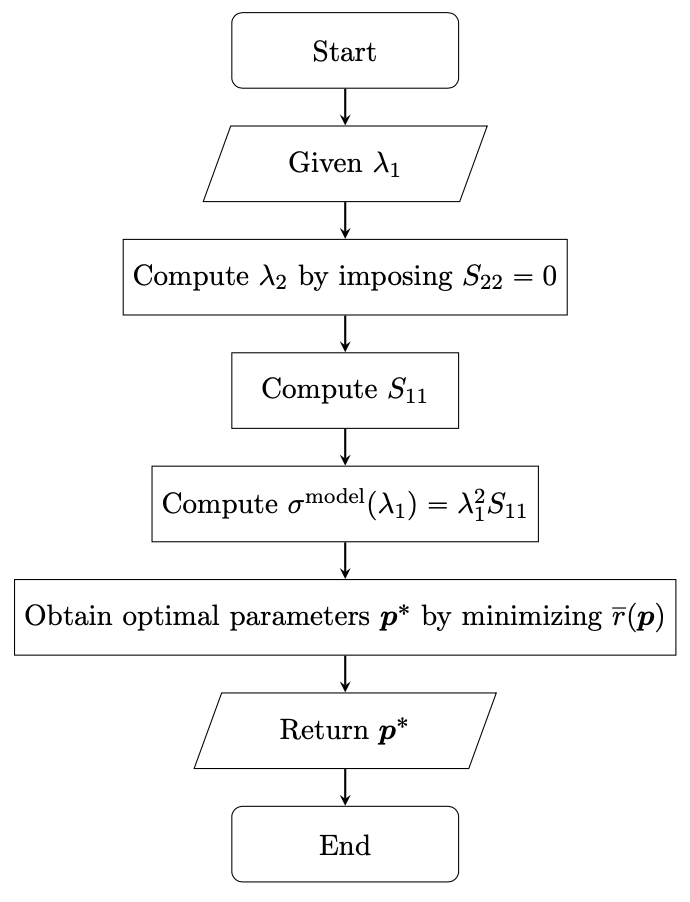
\includegraphics[width = 0.4\textwidth]{Flowchart.png}
    \end{center}
    \caption[Summary of the deterministic calibration.]{Summary of the procedure enabling the deterministic calibration of material parameters on the synthesized samples.}
    \label{fig:flowchart}
\end{figure}
Notice that the optimal values for the parameters involved in the stochastic formulation, gathered in a realization vector $\bfz^*$, are then obtained by using the changes of variables defined in Section \ref{Stochastic Model Homogeneous}.

The results of the adjusted material model and the digitally-generated data for the three layers are shown in Figs.~\ref{fig:det-fit-adv}, \ref{fig:det-fit-med}, and \ref{fig:det-fit-int}. 
\begin{figure}[ht!]
    \begin{center}
        \includegraphics[width = 0.48\textwidth]{Adv_Circ.pdf} \includegraphics[width = 0.48\textwidth]{Adv_Long.pdf}
    \end{center}
    \caption[Fitting results for the adventitia layer.]{Fitting results for the adventitia layer. The reference results are shown in solid black line, while the results obtained with the proposed model are shown in red solid line. Left panel: circumferential direction. Right panel: longitudinal direction.}
    \label{fig:det-fit-adv}
\end{figure}
\begin{figure}[ht!]
    \begin{center}
        \includegraphics[width = 0.48\textwidth]{Med_Circ.pdf} \includegraphics[width = 0.48\textwidth]{Med_Long.pdf}
    \end{center}
    \caption[Fitting results for the media layer.]{Fitting results for the media layer. The reference results are shown in solid black line, while the results obtained with the proposed model are shown in red solid line. Left panel: circumferential direction. Right panel: longitudinal direction.}
    \label{fig:det-fit-med}
\end{figure}
\begin{figure}[ht!]
    \begin{center}
        \includegraphics[width = 0.48\textwidth]{Int_Circ.pdf} \includegraphics[width = 0.48\textwidth]{Int_Long.pdf}
    \end{center}
    \caption[Fitting results for the intima layer.]{Fitting results for the intima layer. The reference results are shown in solid black line, while the results obtained with the proposed model are shown in red solid line. Left panel: circumferential direction. Right panel: longitudinal direction.}
    \label{fig:det-fit-int}
\end{figure}
It is seen that the model can reproduce the data very well, as expected given the similarities between the strain energy density functions used in this paper and in the reference work \cite{holzapfel2005determination} (which only differs in the isotropic contribution). The lists of material parameters thus obtained are provided for all layers in Table~\ref{tab:cal-par-det-adv}, \ref{tab:cal-par-det-med}, and \ref{tab:cal-par-det-int}. The mean averages for these parameters (in the order $\mu_1$, $\mu_2$, $\mu_4$, $\beta_4$, $\alpha$, and $\rho$) are provided for each layer below:
\begin{itemize}
    \item Adventitia: 6.5462 [kPa], 0.1034 [kPa], 21.3557 [kPa], 96.6721 [--], 1.1419 [rad], 0.5151 [--];
    \item Media: 1.2079 [kPa], 0.0230 [kPa], 10.7838 [kPa], 8.1899 [--], 0.3558 [rad], 0.2490 [--];
    \item Intima: 28.4956 [kPa], 0.4725 [kPa], 145.8811 [kPa], 177.3867 [--], 1.1096 [rad], 0.5044 [--].
\end{itemize}

\begin{table}[ht!]
\caption[Calibrated parameters for the adventitia layer.]{Calibrated parameters for the adventitia layer. Specimens numbers are associated with the results presented in \cite{holzapfel2005determination}. Note that the parameter $\mu_4$ here is half of the corresponding parameter in \cite{holzapfel2005determination}, given the expression for the strain energy density function.}
\label{tab:cal-par-det-adv}
\begin{center}
    \begin{tabular}{|c |c| c| c| c| c| c| c|} 
 \hline
 \quad Specimen \quad & \quad $\mu_1$ \quad & \quad $\mu_2$ \quad & \quad $\mu_4$ \quad & \quad $\beta_4$ \quad & \quad $\alpha$ \quad & \quad $\rho$ \quad & Error $\overline{r}(\bfp^*)$ \quad \\
 \quad \# \quad & [kPa] \quad & \quad [kPa] \quad & \quad [kPa] \quad & \quad [--] \quad & \quad [rad] \quad & \quad [--] \quad & $\times 10^{-6}$ \quad \\
 \cline{1-8} 
    1 & 3.8154 & 0.0952   & 16.2516  & 103.8667 & 1.2681 & 0.6503 & 0.3131\\
    2 & 2.2703 & 0.0471   & 6.9480  & 81.3985 & 1.1781 & 0.7510 & 0.8667\\
    3 & 4.8053 & 0.0395   & 33.6126 & 49.4776 & 1.0699 & 0.4999 & 0.1708\\
    5 & 9.1153 & 0.2103   & 41.0040 & 145.0781 & 0.9320 & 0.3998 & 0.8243\\
    6 & 7.7952 & 0.0571   & 12.6815 & 67.9862 & 1.2264 & 0.7003 & 0.1121\\
    8 & 2.0467 & 0.0833   & 18.8116 & 48.7029 & 1.1422 & 0.4040 & 0.2818 \\
    9 & 5.6493 & 0.2089   & 16.4234 & 167.2432 & 1.3151 & 0.2998 & 0.2761\\
    10 & 14.7392 & 0.0778 & 59.5418 & 214.0337 & 0.9320 & 0.6001 & 0.2067\\
    11 & 12.3502 & 0.1629 & 17.5735 & 84.9840 & 1.2083 & 0.6005 & 0.2450\\
    12 & 2.8631 & 0.1009  & 8.7606 & 68.4434 & 0.9597 & 0.4105 & 0.9009\\
    13 & 6.5583 & 0.0541  &  3.3039 & 32.1794 & 1.3297 & 0.3500 & 0.2420\\
 \hline 
\end{tabular}
\end{center}
\end{table}

\begin{table}[ht!]
\caption[Calibrated parameters for the media layer.]{Calibrated parameters for the media layer. Specimens numbers are associated with the results presented in \cite{holzapfel2005determination}. Note that the parameter $\mu_4$ here is half of the corresponding parameter in \cite{holzapfel2005determination}, given the expression for the strain energy density function.}
\label{tab:cal-par-det-med}
\begin{center}
    \begin{tabular}{|c |c| c| c| c| c| c| c|} 
 \hline
 \quad Specimen \quad & \quad $\mu_1$ \quad & \quad $\mu_2$ \quad & \quad $\mu_4$ \quad & \quad $\beta_4$ \quad & \quad $\alpha$ \quad & \quad $\rho$ \quad & Error $\overline{r}(\bfp^*)$ \quad \\
 \quad \# \quad & [kPa] \quad & \quad [kPa] \quad & \quad [kPa] \quad & \quad [--] \quad & \quad [rad] \quad & \quad [--] \quad & $\times 10^{-6}$ \quad \\
 \cline{1-8}
    1 & 0.9122 & 0.0094  & 6.6063  & 10.7580 & 0.3592 & 0.2476 & 0.2793\\
    2 & 1.0174 & 0.0269  & 12.8334  & 5.8988 & 0.4449 & 0.2970 & 0.2268\\
    3 & 1.7214 & 0.0236  & 10.4581  & 5.7353 & 0.3916 & 0.1967 & 0.2478\\
    4 & 1.5992 & 0.0109  &  13.1523 & 9.5337 & 0.4439 & 0.3980 & 0.1677\\
    5 & 2.4868 & 0.0223  & 8.3441  & 13.8411 & 0.2968 & 0.2000 & 0.2959\\
    6 & 0.6409 & 0.0338  & 15.2760  & 5.3399 & 0.3226 & 0.2987 & 0.2007\\
    7 & 0.8698 & 0.0246  & 12.4674  & 7.5124 & 0.2147 & 0.1500 & 0.2853\\
    8 & 0.2368 & 0.0313  &  13.9616 & 5.4142 & 0.1840 & 0.1993 & 0.1661\\
    9 & 2.2856 & 0.0119  &  4.2552  & 12.8970 & 0.4405 & 0.3032 & 0.1334\\
    10 & 0.7071 & 0.0531 & 15.5753 & 2.5561 & 0.2740 & 0.0986 & 0.1921\\
    11 & 1.1838 & 0.0117 & 6.5073 & 8.4201 & 0.5203 & 0.3015 & 0.3128\\
    12 & 0.8871 & 0.0263 & 10.7400 & 7.7343 & 0.3482 & 0.1480 & 0.2638\\
    13 & 1.1550 & 0.0130 & 10.0128 & 10.8277 & 0.3842 & 0.3984 & 0.2561\\
 \hline
\end{tabular}
\end{center}
\end{table}

\begin{table}[ht!]
\caption[Calibrated parameters for the intima layer.]{Calibrated parameters for the intima layer. Specimens numbers are associated with the results presented in \cite{holzapfel2005determination}. Note that the parameter $\mu_4$ here is half of the corresponding parameter in \cite{holzapfel2005determination}, given the expression for the strain energy density function.}
\label{tab:cal-par-det-int}
\begin{center}
    \begin{tabular}{|c |c| c| c| c| c| c| c|} 
 \hline
 \quad Specimen \quad & \quad $\mu_1$ \quad & \quad $\mu_2$ \quad & \quad $\mu_4$ \quad & \quad $\beta_4$ \quad & \quad $\alpha$ \quad & \quad $\rho$ \quad & Error $\overline{r}(\bfp^*)$ \quad \\
 \quad \# \quad & [kPa] \quad & \quad [kPa] \quad & \quad [kPa] \quad & \quad [--] \quad & \quad [rad] \quad & \quad [--] \quad & $\times 10^{-6}$ \quad \\
 \cline{1-8} 
   1 & 26.0930 &   1.0707 &  61.8350 & 180.6829  &  1.2129 &   0.5496 &  0.1064\\
   2 & 42.0952 &   0.1300 & 132.1545 & 286.9763  &  0.9372  &  0.6999 & 0.0253\\
   3 & 24.8050 &   0.2085 & 117.1730 & 176.7649  &  1.0085  &  0.5005 & 0.0233\\
   4 & 48.1296 &   2.2548 & 930.3108 & 454.7669  &  0.8168  &  0.3994 & 0.0235\\
   5 & 24.2734 &   0.1897 & 184.8636 & 342.9503  &  0.6965  &  0.7002 & 0.0266\\
   7 & 34.2402 &   0.1682  & 27.4200 &  92.7600  &  1.2620  &  0.3498 & 0.0307\\
   8 & 25.8023 &   0.1473  & 30.0657 & 110.3671  &  1.2950  &  0.3499 & 0.0253\\
   10 & 27.2055 &   0.1071 &  16.2175 &  72.3563  &  1.1521  &  0.3998 & 0.0223\\
   11 & 25.8057 &   0.1510 &  28.1253  & 77.8412  &  1.1570  &  0.4999 & 0.0256\\
   12 & 15.2380 &   0.5128 &  40.1371 &  73.7906  &  1.3643  &  0.6499 & 0.0203\\
   13 & 19.7643 &   0.2577 &   36.3891 &  81.9973 &   1.3036  &  0.4498 & 0.0263\\
 \hline 
\end{tabular}
\end{center}
\end{table}


\subsection{Calibration of the Stochastic Model} \label{subsec:sto-calibration}

Since the components of $\bfZ$ are statistically independent, we use the maximum likelihood method to calibrate the hyperparameters for each random variable. Denote by $\boldsymbol{s}$ the vector gathering the set of hyperparameters for a given component of $\bfZ$ in the stochastic model. The optimal value of $\boldsymbol{s}$ is then obtained as
\begin{align}
    \hat{\boldsymbol{s}} &= \text{argmax}_{\boldsymbol{s} \in \mathcal{C}_{\boldsymbol{s}}} \quad \mathcal{L}(\boldsymbol{s}; \bfy)\,,
\end{align}
where $\mathcal{C}_{\boldsymbol{s}}$ denotes the parameter space, $\mathcal{L}$ is the likelihood function, and $\bfy$ is the observed data sample. The values of all hyperparameters are given in Table~\ref{tab:hyperparameters}, and the associated probability density functions (together with samples) are shown in Figs.~\ref{fig:MLE-Set-1}, \ref{fig:MLE-Set-2}, and \ref{fig:MLE-Set-3}.
\begin{table}[ht!]
\caption[Hyperparameters estimated with the maximum likelihood method.]{Hyperparameters estimated with the maximum likelihood method for all layers.}
\label{tab:hyperparameters}
\begin{center}
    \begin{tabular}{|c|c|c|c|} 
 \hline
 \quad Parameter \quad & \quad $\hat{\boldsymbol{s}}$ (adventitia) \quad & \quad $\hat{\boldsymbol{s}}$ (media) \quad & \quad $\hat{\boldsymbol{s}}$ (intima) \quad \\
 \cline{1-4} 
    $C_2$ & $(2.9459, 4.6266)$  & $(3.6841, 0.7075)$   & $(1.4120, 35.8575)$\\
    $V$   & $(1.6574, 99.5985)$ & $(5.9044, 22.4244)$  & $(0.6364, 1.645 \times 10^3)$\\
    $B_4$ & $(3.5262, 27.4153)$ & $(5.2736, 1.5154)$   & $(1.1744, 129.0230)$\\
    $U$   & $(48.4729, 2.5140)$ & $(14.4793, 1.1649)$  & $(34.4290, 1.43553)$\\
    $R$   & $(5.8703, 5.5101)$  & $(6.25578, 19.3627)$ & $(3.1868, 1.9178)$\\
    $T$   & $(17.7955, 6.6881)$ & $(8.8830, 30.5876)$  & $(4.5830, 5.2297)$\\
 \hline 
\end{tabular}
\end{center}
\end{table}
In practice, these hyperparameters can used to generate mathematically-consistent virtual samples. 

\begin{figure}[ht!]
    \begin{center}
        \includegraphics[width = 0.48\textwidth]{MLE-C2.pdf} \includegraphics[width = 0.48\textwidth]{MLE-V.pdf}
    \end{center}
    \caption[Probability density functions (PDFs) of $C_2$ and $V$.]{Probability density functions (PDFs), with hyperparameters estimated with the maximum likelihood method, and experimental samples. Left panel: random variable $C_2$. Right panel: random variable $V$.}
    \label{fig:MLE-Set-1}
\end{figure}
\begin{figure}[ht!]
    \begin{center}
        \includegraphics[width = 0.48\textwidth]{MLE-B4.pdf} \includegraphics[width = 0.48\textwidth]{MLE-U.pdf}
    \end{center}
    \caption[Probability density functions (PDFs) of $B_2$ and $U$.]{Probability density functions (PDFs), with hyperparameters estimated with the maximum likelihood method, and experimental samples. Left panel: random variable $B_2$. Right panel: random variable $U$.}
    \label{fig:MLE-Set-2}
\end{figure}
\begin{figure}[ht!]
    \begin{center}
        \includegraphics[width = 0.48\textwidth]{MLE-T.pdf} \includegraphics[width = 0.48\textwidth]{MLE-R.pdf}
    \end{center}
    \caption[Probability density functions (PDFs) of $T$ and $R$.]{Probability density functions (PDFs), with hyperparameters estimated with the maximum likelihood method, and experimental samples. Left panel: random variable $T$. Right panel: random variable $R$.}
    \label{fig:MLE-Set-3}
\end{figure}

Using these results, new samples of $\bfZ$ can be generated and pulled back to obtain samples of the primary parameters defining the strain energy density function. Using $10^{6}$ samples, the following mean values were obtained for these parameters:
\begin{itemize}
    \item Adventitia: 6.4760 [kPa], 0.1297 [kPa], 24.0164 [kPa], 96.4960 [--], 1.1426 [rad], 0.5172 [--];
    \item Media: 1.2076 [kPa], 0.0379 [kPa], 11.1438 [kPa], 8.0084 [--], 0.3539 [rad], 0.2440 [--];
    \item Intima: 24.2965 [kPa], 0.3893 [kPa], 136.2482 [kPa], 151.3538 [--], 0.9806 [rad], 0.4672 [--].
\end{itemize}
It is seen that these results slightly differ from the ones reported in Section \ref{subsec:det-calibration}, where mean averaging was used instead of a maximum likelihood estimator. In order to qualitatively assess this result, the mean responses obtained by using either parameterization (that is, the one provided in Section \ref{subsec:det-calibration} or the one given above) are shown for all layers and both directions in Figs.~\ref{fig:mean-adv}, \ref{fig:mean-med}, and \ref{fig:mean-int}. The difference between the two responses is most noticeable for the intima layer, due to the strong stiffening effect. Finally, 95\% confidence intervals were estimated with the model, using 100,000 independent samples. These intervals are also displayed in Figs.~\ref{fig:mean-adv}, \ref{fig:mean-med}, and \ref{fig:mean-int}, and are seen to capture experimental variability with reasonable accuracy.
\begin{figure}[ht!]
    \begin{center}
        \includegraphics[width = 0.48\textwidth]{MeanCI-Adv-Circ.pdf} \includegraphics[width = 0.48\textwidth]{MeanCI-Adv-Long.pdf}
    \end{center}
    \caption[Experimental results obtained for the adventitia layer.]{Experimental results (black solid lines), mean responses obtained for the adventitia layer by using either the MLE-based estimate (blue solid line) or a mean average (blue dashed line), and 95\% confidence interval (red solid line). Left panel: circumferential direction. Right panel: longitudinal direction.}
    \label{fig:mean-adv}
\end{figure}
\begin{figure}[ht!]
    \begin{center}
        \includegraphics[width = 0.48\textwidth]{MeanCI-Med-Circ.pdf} \includegraphics[width = 0.48\textwidth]{MeanCI-Med-Long.pdf}
    \end{center}
    \caption[Experimental results obtained for the media layer.]{Experimental results (black solid lines), mean responses obtained for the media layer by using either the MLE-based estimate (blue solid line) or a mean average (blue dashed line), and 95\% confidence interval (red solid line). Left panel: circumferential direction. Right panel: longitudinal direction.}
    \label{fig:mean-med}
\end{figure}
\begin{figure}[ht!]
    \begin{center}
        \includegraphics[width = 0.48\textwidth]{MeanCI-Int-Circ.pdf} \includegraphics[width = 0.48\textwidth]{MeanCI-Int-Long.pdf}
    \end{center}
    \caption[Experimental results obtained for the intima layer.]{Experimental results (black solid lines), mean responses obtained for the intima layer by using either the MLE-based estimate (blue solid line) or a mean average (blue dashed line), and 95\% confidence interval (red solid line). Left panel: circumferential direction. Right panel: longitudinal direction.}
    \label{fig:mean-int}
\end{figure}

\section{Uncertainty Propagation} \label{sec:uncertainty-propagation}


\subsection{Definition of the Random Field Model on a Patient-Specific Geometry}

In this section, we consider the propagation of the uncertainties associated with the proposed random field model on a patient-specific geometry. Without loss of generality, we assume that the latter corresponds to the adventitia layer (which is the outermost layer in the arterial wall). We use the domain studied in \cite{STABER201894}, which was obtained by postprocessing the inner surface available as file 0098 in the Aneurisk database \cite{AneuriskWeb}. The domain is about $12$ [mm] long and is shown in Fig.~\ref{fig:geometry}. Details about discretization are provided in Section \ref{subsec:SFEM-propagation}.
\begin{figure}[ht!]
    \begin{center}
        \includegraphics[trim = {5cm 7cm 5cm 7cm}, clip, width = 0.48\textwidth]{Artery3D.pdf} \includegraphics[trim = {5cm 5cm 5cm 7cm}, clip, width = 0.4\textwidth]{ArterySlice.pdf}
    \end{center}
    \caption[Three-dimensional and slice views of the arterial wall.]{Three-dimensional and slice views of the arterial wall, computed from \cite{AneuriskWeb}.}
    \label{fig:geometry}
\end{figure}

In order to define the latent Gaussian field $\{{\bf \Xi}(\bfx), \bfx \in B\}$, we use the SPDE approach introduced in Section \ref{subsec:def-Gaussian} (with $\alpha = 2$). As a preliminary step, we use the Laplace-Dirichlet Rule-Based algorithm \cite{Bayer2012,Augustin2014} to define some local orientation fields involved in the parameterization of the diffusion $[H]$. Specifically, we introduce the vector fields $\bfx \mapsto \bfe^{(1)}(\bfx)$ and $\bfx \mapsto \bfe^{(2)}(\bfx)$ defined as
\begin{equation}
\bs{e}^{(1)}(\bs{x}) = \frac{\nabla\Psi_2(\bs{x})}{ \| \nabla \Psi_2(\bs{x}) \| }~, \quad \bs{e}^{(2)}(\bs{x}) = \bs{e}^{(3)}(\bs{x}) \times \bs{e}^{(1)}(\bs{x})~, \quad \bs{e}^{(3)}(\bs{x}) = \frac{\nabla \Psi_1(\bs{x})}{ \| \nabla \Psi_1(\bs{x}) \| }~,
\end{equation}
where $\bs{x} \mapsto \Psi_1(\bs{x})$ satisfies 
\begin{equation}
\Delta \Psi_1({\bs{x}}) = 0~, \quad \forall \, {\bs{x}} \in B~,
\end{equation}
with $\Psi_1({\bs{x}}) = 0$ on the inlet surface and $\Psi_1({\bs{x}}) = 1$ on the outlet surface, and $\bs{x} \mapsto \Psi_2(\bs{x})$ is the solution to a similar Laplace problem with $\Psi_2({\bs{x}}) = 0$ on the inner surface and $\Psi_2({\bs{x}}) = 1$ on the outer surface \cite{STABER201894}.

As a first step, we then consider the Gaussian component associated with the angle random field $\{A(\bfx), \bfx \in B\}$ and use a SPDE where the diffusion field is defined as
\begin{equation}\label{eq:def-H-final-application}
    \bs{D}(\bfx) = \kappa \bs{I} + \tau_1 \hat{\bfe}^{(1)}(\bfx) \otimes \hat{\bfe}^{(1)}(\bfx) + \tau_2 \hat{\bfe}^{(2)}(\bfx) \otimes \hat{\bfe}^{(2)}(\bfx)\,,
\end{equation}
where
\begin{equation}    
    \hat{\bfe}^{(1)}(\bfx) = \cos(\underline{a}) \bfe^{(1)}(\bfx) + \sin(\underline{a})\bfe^{(2)}(\bfx)\,, \quad \hat{\bfe}^{(2)}(\bfx) = \cos(\underline{a}) \bfe^{(1)}(\bfx) - \sin(\underline{a})\bfe^{(2)}(\bfx)\,,
\end{equation}
and $\underline{a}$ is the mean value for the angle obtained from the calibrated step detailed in Section \ref{sec:calibration} (for the adventitia layer). In effect, this introduces some waviness effect in the local orientation, for both the anisotropic mechanical behavior and covariance structure, which can be related to waviness in the orientation of collagen fibers at a finer scale. By construction, this modeling feature can be turned off by setting the associated coefficient of variation to zero.

Next, and for a \textit{given} sample $\bfx \mapsto a(\bfx, \theta)$ of the angle random field thus obtained, with $\theta \in \Theta$, the latent Gaussian components associated with the other material random fields are defined and sampled by solving the SPDE with the diffusion taken as in Eq.~\eqref{eq:def-H-final-application}, where the orientation vectors are now defined as
\begin{equation}    
    \hat{\bfe}^{(1)}(\bfx) = \cos(a(\bfx, \theta)) \bfe^{(1)}(\bfx) + \sin(a(\bfx, \theta))\bfe^{(2)}(\bfx)
\end{equation}
and
\begin{equation}    
 \hat{\bfe}^{(2)}(\bfx) = \cos(a(\bfx, \theta)) \bfe^{(1)}(\bfx) - \sin(a(\bfx, \theta))\bfe^{(2)}(\bfx)\,.
\end{equation}

Following the methodology of construction presented in Section \ref{sec:sto-heterogeneous}, we now proceed with the specification of the hyperparameters defining the transport map $H$. A natural choice here is to use the parameters identified in Section \ref{subsec:sto-calibration}; see Table~\ref{tab:hyperparameters}. However, the associated probability density functions represent inter-patient variability and would therefore generate unrealistically large (intra-patient) spatial fluctuations. For this reason, we propose to preserve the mean values estimated at the calibration stage, and to scale the coefficients of variation in a proportional manner (meaning that properties that exhibit larger fluctuations still present larger spatial variations). The proposed values for these coefficients of variation are listed in Table~\ref{tab:scaled-hyperparameters}.
\begin{table}[ht!]
\caption[Scaled coefficients of variation of the random variables.]{Scaled values for the coefficients of variation of the random variables.}
\label{tab:scaled-hyperparameters}
\begin{center}
    \begin{tabular}{|c|c|c|} 
 \hline
 \quad Parameter \quad & \quad Data-based coefficient of variation \quad & \quad Scaled coefficient of variation \quad \\
 \cline{1-3} 
    $C_2$ & $0.5826$  & $0.15$ \\
    $V$   & $0.7768$ & $0.2$ \\
    $B_4$ & $0.5325$ & $0.1371$ \\
    $U$   & $0.0316$ & $0.0081$ \\
    $R$   & $0.2753$  & $0.0709$ \\
    $T$   & $0.1214$ & $0.0313$ \\
 \hline 
 \end{tabular}
\end{center}
\end{table}
The corresponding set of hyperparameters are provided in Table~\ref{tab:hyperparameters-scaled}.
\begin{table}[ht!]
\caption[Hyperparameters corresponding to the scaled coefficients of variation.]{Hyperparameters corresponding to the scaled coefficients of variation (given in the far-right column in Table~\ref{tab:scaled-hyperparameters}).}
\label{tab:hyperparameters-scaled}
\begin{center}
    \begin{tabular}{|c|c|} 
 \hline
 \quad Parameter \quad & \quad $\hat{\boldsymbol{s}}$ (adventitia) \quad \\
 \cline{1-2} 
    $C_2$ & $(44.4351, 0.3067)$\\
    $V$   & $(25, 6.6031)$\\
    $B_4$ & $(53.1877, 1.8176)$\\
    $U$   & $(744.5323, 38.6146)$\\
    $R$   & $(95.81, 89.9306)$\\
    $T$   & $(278.6547, 104.727)$\\
 \hline 
\end{tabular}
\end{center}
\end{table}

Realizations of the random fields of material parameters are shown in Figs.~\ref{fig:samples-1}, \ref{fig:samples-2}, and \ref{fig:samples-3}, for $\gamma = 1$, $\kappa = 0.1$, and $\tau_1 = \tau_2 = 10$. These values are selected for the sake of illustration to induce moderate correlation ranges on the arterial wall. The identification of such parameters requires spatial data that are not currently available for the proposed application (and may be obtained using, e.g., ultrasound characterization techniques) and is left for future work.
\begin{figure}[ht!]
    \begin{center}
        
    \includegraphics[trim = {6cm 3cm 6cm 5cm}, clip, width = 0.48\textwidth]{Sample_G1.pdf} \includegraphics[trim = {6cm 3cm 6cm 5cm}, clip, width = 0.48\textwidth]{Sample_G2.pdf}
    \end{center}
    \caption[Sample of $\{G_1(\bfx), \bfx \in B\}$ and $\{G_2(\bfx), \bfx \in B\}$ in the adventitia layer.]{Sample of $\{G_1(\bfx), \bfx \in B\}$ (left) and $\{G_2(\bfx), \bfx \in B\}$ (right) in the adventitia layer.}
    \label{fig:samples-1}
\end{figure}

\begin{figure}[ht!]
    \begin{center}
        \includegraphics[trim = {6cm 3cm 6cm 5cm}, clip, width = 0.48\textwidth]{Sample_G4.pdf} \includegraphics[trim = {6cm 3cm 6cm 5cm}, clip, width = 0.48\textwidth]{Sample_B4.pdf}
    \end{center}
    \caption[Sample of $\{G_4(\bfx), \bfx \in B\}$ and $\{B_4(\bfx), \bfx \in B\}$ in the adventitia layer.]{Sample of $\{G_4(\bfx), \bfx \in B\}$ (left) and $\{B_4(\bfx), \bfx \in B\}$ (right) in the adventitia layer.}
    \label{fig:samples-2}
\end{figure}

\begin{figure}[ht!]
    \begin{center}
        \includegraphics[trim = {6cm 3cm 6cm 5cm}, clip, width = 0.48\textwidth]{Sample_R.pdf} \includegraphics[trim = {6cm 3cm 6cm 5cm}, clip, width = 0.48\textwidth]{Sample_A.pdf}
    \end{center}
    \caption[Sample of $\{R(\bfx), \bfx \in B\}$ and $\{A(\bfx), \bfx \in B\}$ in the adventitia layer.]{Sample of $\{R(\bfx), \bfx \in B\}$ (left) and $\{A(\bfx), \bfx \in B\}$ (right) in the adventitia layer.}
    \label{fig:samples-3}
\end{figure}

\subsection{Propagation of Uncertainties}\label{subsec:SFEM-propagation}

In this work, the nonlinear boundary value problem is solved by the finite element method, using a total Lagrangian formulation and a three-field formulation ($\mathbb{P}_2$-$\mathbb{P}_0$-$\mathbb{P}_0$ discretization) to handle quasi-incompressibility \cite{wriggers2008nonlinear}. The geometry shown in Fig.~\ref{fig:geometry} is discretized with a mesh containing $297,828$ cells and $432,250$ nodes. An inflating pressure of 1 [kPa] is applied on the inner layer and sliding displacement boundary conditions are prescribed on the inlet and outlet surfaces (the system is made statically determined by restricting additional degrees of freedom at two nodes located on the outlet surface). Implementation was performed within the MOOSE finite element framework \cite{permann2020moose} and code verification was conducted through the method of manufactured solution (described in \ref{app:VV-artery}).  

Given the random field modeling setting, a Monte-Carlo approach was used to propagate uncertainties (see the remark at the end of this section). Interested readers are referred to \cite{Ghanem2017} for a comprehensive review on alternative stochastic solvers (see \cite{hauseux2018quantifying} for a specific discussion regarding hyperelastic materials). Parallel computing with 36 cores was used to accelerate the deterministic runs.

The fields of mean values and coefficients of variation are shown in Fig.~\ref{fig:vonMises}.
\begin{figure}[ht!]
    \begin{center}
        \includegraphics[trim = {6cm 3cm 6cm 5cm}, clip, width = 0.48\textwidth]{Mean-vMStress.pdf} \includegraphics[trim = {6cm 3cm 6cm 5cm}, clip, width = 0.48\textwidth]{CV-vMStress.pdf}
    \end{center}
    \caption[Mean and coefficient of variation for the von Mises stress.]{Mean (left) and coefficient of variation (right) for the von Mises stress (slice views).}
    \label{fig:vonMises}
\end{figure}
Substantial spatial variations are observed in both fields and localization is less pronounced than in the results presented in \cite{STABER201894}---as angular waviness tends to mitigate that effect. Values for the mean field range from 0.15 to 40 [kPa], while values for the coefficient of variation are distributed between 0.025 to 0.42. While these quantitative results are conditioned by the proposed scaling in variance (defined in Tab.~\ref{tab:scaled-hyperparameters}) and the selected values for the hyperparameters defining the latent Gaussian fields, they show the impact of material variability on the response of the arterial wall. Additional work assimilating spatial data is therefore necessary to refine the propagation analysis and translate the results into practical applications: the proposed modeling framework is a first step towards that goal.

\begin{remark}
The usual spectral approach to uncertainty propagation consists in representing the random fields through Karhunen-Lo\`eve expansions and in seeking a polynomial chaos surrogate in terms of the reduced variables. It is therefore instructive to analyze a posteriori the dimension obtained for a given field defined and sampled through the SPDE approach, say $\{G_1(\bfx), \bfx \in B\}$. The graph of the standard error function $n \mapsto \textnormal{Conv}(n)$, where
\begin{equation}
    \textnormal{Conv}(n) = 1 - \frac{\sum_{i = 1}^{n} \lambda_i}{\textnormal{tr}(\textnormal{Cov}\{G_1\})}
\end{equation}
and the covariance matrix $\textnormal{Cov}\{G_1\}$ (and its eigenvalues $\{\lambda_i\}_{i \geq 1}$) are computed by using a singular value decomposition on the matrix of centered samples (200 samples are used here), is shown in Fig.~\ref{fig:conv}.
\begin{figure}[ht!]
    \begin{center}
        \includegraphics[width = 0.5\textwidth]{ConvN.pdf}
    \end{center}
    \caption[Graph of the function $n \mapsto \textnormal{Conv}(n)$.]{Graph of the function $n \mapsto \textnormal{Conv}(n)$.}
    \label{fig:conv}
\end{figure}
Retaining a truncation threshold of $0.01$ leads to a reduced dimension of 158, which suggests---given that six random fields are involved in the parameterization of the stochastic strain energy density function---a very high-dimensional setting for propagation through collocation-type approaches.
\end{remark} % A regular chapter, starts with '\chapter{Title}'
\chapter{Polyconvex Neural Networks for Hyperelastic Constitutive Models: A Rectification Approach}
\label{chap:polyconvex}

Constitutive models based on neural networks (NN) have received growing attention over the past few years, owing to their ability to represent nonlinear mappings in a high dimensional setting. There is a very substantial amount of papers published on this topic, for a wide variety of material behaviors; see, \textit{e.g.},  \cite{flaschel2021unsupervised,xu2021learning,holzapfel2021predictive,jung2006neural,ghaboussi1998autoprogressive,ghaboussi1998new,hashash2004numerical,furukawa1998implicit,joshi2022bayesian,as2022mechanics,Asad-IJNME,KLEIN2022104703} and the references therein, in a non-exhaustive manner.

Beyond classical data science aspects that pertain to architecture design, training and validation strategies, and the analysis of approximation capabilities, a central concern is to make such surrogates amenable to scientific simulations where such models are typically set to parameterize systems of partial differential equations. In this context, the surrogate must satisfy both physical assumptions and mathematical properties (\textit{e.g.}, boundedness or a certain type of convexity) to ensure the existence (and potentially, the uniqueness) of solutions. 
In the case of nonlinear elasticity for instance, a strain energy density function is theoretically required to satisfy frame indifference, some asymptotic behavior, and specific convexity and growth conditions. There are various ways to enforce such properties and in particular, the convexity requirement. The simplest strategy consists in using some unconstrained neural network that, if properly calibrated on a rich enough dataset, may possess desired convexity. Another way to enforce convexity is to add a penalty term in the loss function during the training stage; see, \textit{e.g.}, \cite{liu2020generic}. This latter strategy corresponds to a weak enforcement and hence does not prevent from checking the condition \textit{a posteriori}. 

In this work, we consider enforcing convexity in the strong sense, by defining classes of surrogate models that satisfy the condition \textit{a priori}. The issue of ensuring the convexity of a neural network is not new and was mostly tackled by constraining the network through the use of non-negative weights and convex activation functions \cite{amos2017input}. Restriction on weights can be imposed by constraining the weights during training, or by using a mapping from $\mathbb{R}$ into $\mathbb{R}_{\geq 0}$ that acts on unconstrained weights \cite{sivaprasad2021curious,Asad-IJNME}. Applications in computational mechanics are presented in \cite{masi2021thermodynamics, as2022mechanics,Asad-IJNME} for example. A detailed analysis about the use of constrained neural networks for polyconvex anisotropic hyperelastic models can be found in \cite{KLEIN2022104703}, in particular.

Here, we aim to construct a convex neural network model without affecting expressiveness (that is, without constraining weights \textit{a priori}) and training cost (which can be affected by transformations performed on weights at the training stage). Building upon recent works on monotonic neural networks \cite{wehenkel2019unconstrained} and monotone transport maps for density estimation \cite{baptista2020adaptive}, our approach relies on simple integral representations to define an operator that transforms any arbitrary function (and in particular, a \textit{free} neural network) into a convex function. This strategy thus entails the rectification of the whole neural network model. We show, through various numerical experiments on both digitally synthesized and experimental datasets, that the proposed rectified models enable proper fitting. They are also seen to converge much faster than constrained models (in terms of number of iterations)---at the expense of an increased computational cost per iteration. 

The rest of this section is organized as follows. The mechanistic parameterization and rectification strategy are first presented in Section~\ref{sec:rectifiers} (together with a toy example). Applications to standard hyperelastic models relevant to both isotropic and anisotropic materials are then discussed in Section \ref{sec:applications}.

\section{Rectified Neural Network Representations}
\label{sec:rectifiers}

\subsection{Background in Elasticity}
Let $\Omega$ be a collection of material points identified with their vector of coordinates $\bfX$ in $\mathbb{R}^3$, and denote by $\partial \Omega$ the boundary of $\Omega$. For any material point $\bfX \in \Omega$, the spatial point $\bfx$ in the deformed configuration $\Omega^\varphi$ is given by $\bfx = \varphi (\bfX)$, where $\varphi$ is the deformation map. For any $\bfX \in \Omega$, the deformation gradient $\defgrad$ is a second-order tensor defined as $\defgrad = \grad_{\bfX} \bfx$. The left and right Cauchy-Green deformation tensors are given by $\bfB = \defgrad \defgrad^T$ and $\rcg = \defgrad^T \defgrad$, respectively.

We seek to construct a neural network surrogate that satisfies physical axioms and mathematical requirements arising in existence theorem in finite elasticity. From a theoretical standpoint, strain energy density functions are required to satisfy \cite{ciarlet1988mathematical,truesdell2004non}:
\begin{enumerate}
    \item Principle of material frame indifference (objectivity), stated as: $\forall \bfQ \in \mathrm{SO}(3)$,
    \begin{equation}
            w(\bfQ \bfF) = w(\bfF)\,, \quad \bfP(\bfQ \bfF) = \bfQ \bfP(\bfF)\,,
    \end{equation}
    where $\bfP$ is the first Piola-Kirchhoff stress tensor;
    \item Proper convexity conditions; 
    \item Some asymptotic behavior as $\det (\bfF) \to 0^+$; and
    \item A coerciveness inequality (growth conditions).
\end{enumerate}
In particular, the requirements (2--4) are fundamental to ensure the existence of (at least) one minimizer for the energy functional, see Chapter 7 in \cite{ciarlet1988mathematical} (see also \cite{pedregal2000variational,Dacorogna1989}).

Material frame-indifference is, in general, achieved by defining $w$ in terms of the right Cauchy-Green deformation tensor $\bfC$, which is an \textit{a priori} objective kinematic variable \cite{truesdell2004non}. Following the work by Ball \cite{ball1976convexity}, polyconvexity is often imposed in lieu of convexity, as (i) it does not conflict with any physical constraints; (ii) it is generally satisfied by commonly employed models; and (iii) it enables the derivation of powerful existence results \cite{ciarlet1988mathematical}. To proceed with the construction of the model, it is instructive at this point to recall the definition of polyconvexity. A strain energy density function $w:\mathbb{M}_+^3 \to \mathbb{R}$ is polyconvex if there exists a convex function $w^*:\mathbb{M}^3 \times \mathbb{M}^3 \times \mathbb{R}$ such that
\begin{equation}  
    w(\bfF) = w^*(\bfF, \mathrm{Cof}(\bfF), \det(\bfF))\,, 
\end{equation}
for all $\bfF \in \mathbb{M}_+^3$, where (i) $\mathrm{Cof}(\bfF)$ and $\det(\bfF)$ are the cofactor matrix and determinant of $\bfF$; (ii) $\mathbb{M}^3$ and $\mathbb{M}_+^3$ denote the sets of real square matrices of order $3$ with arbitrary and strictly positive determinants, respectively. The requirements (3) and (4) above, related to volume annihilation and coercivity, are crucial in the analytical derivation of functional forms for $w$. They are, however, less relevant to surrogate modeling which only involves bounded intervals, by construction. In this context, the choice of a proper parameterization (in terms of $\bfC$) and the satisfaction of the polyconvexity requirement are sufficient to ensure well-posedness and physical consistency. 

Following the previous discussion, we then consider the construction of a polyconvex surrogate, that is $w(\bfC) = w^*(I_1, I_2, I_3)$
% \begin{equation}
%     w(\bfC) = w^*(I_1, I_2, I_3)
% \end{equation}
owing to a slight abuse of notation, where $I_1 = \tr \bfC$, $I_2 = \tr [ \mathrm{Cof}\,\bfC ]$, and $I_3 = \det \bfC$ are the polyconvex invariants of the right Cauchy-Green tensor $\bfC$. We assume an additive decomposition and define $w^*$ as
\begin{equation}
    w^*(I_1, I_2, I_3) := \sum_{i = 1}^{3} w_i^*(I_i)\,,
\end{equation}
where $\{w_i^*\}_{i = 1}^3$ are convex in the associated variables, hence ensuring the polyconvexity of $w^*$ \cite{hartmann2003polyconvexity,schroder2003invariant}. Notice that the above formulation can readily be extended to model anisotropic behaviors, by including mixed invariants that involve structural tensors \cite{ebbing2010construction} (see Sections \ref{subsec:anisotropic-app} and \ref{subsec:exp-app}). 

Our aim now is to construct the set of convex functions $\{w_i^*\}_{i = 1}^3$ using \textit{fully unconstrained} neural networks. %To that end, we invoke the integral representation for convex functions, as detailed in the next section.

\subsection{Rectification of Unconstrained Neural Networks for Constitutive Modeling in Finite Elasticity}
\label{subsec:rectification}
In order to define the functions $\{w_i^*\}_{i = 1}^3$, we start by recalling the integral representation of convex functions, using generic notation. 

Let $f:I \to \mathbb{R}$ be a convex function. Then $f$ admits the representation
\begin{equation}\label{eq:Rec-Con}
    f(x) = f(a) + \int_a^x \phi(t)\,dt\,,
\end{equation}
for $a < x$ in the interval $I$, where $\phi:I \to \mathbb{R}$ is a nondecreasing function. The constant $f(a)$ in the right-hand side of Eq.~\eqref{eq:Rec-Con} can be derived by fixing the value of $f$ at some point $x^\star \geq a$ in $I$, that is
\begin{equation}\label{eq:Rec-Con-Value}
    f(a) = f(x^\star) - \int_a^{x^\star} \phi(t)\,dt\,.
\end{equation}
In the case of a strain energy density function, the point $x^\star$ is associated with the normalization condition $w(\bfI) = 0$.

The central idea is to define $\phi$ in terms of an arbitrary function, soon to be taken as an unconstrained NN. In order to enforce the monotonicity of $\phi$, we rely on the representation proposed in \cite{baptista2020adaptive} to enforce monotonicity on transport maps. Specifically, we define $\phi$ as
\begin{equation}\label{eq:Rec-Inc}
    \phi(t) := \Phi(0) + \int_{0}^{t} g\left(\frac{d\Phi(z)}{dz}\right)\,dz\,,
\end{equation}
where $\Phi:\mathbb{R} \to \mathbb{R}$ is \textit{any} smooth function and $g:\mathbb{R} \to \mathbb{R}_{\geq 0}$ is a positive function. The operator defined by Eq.~\eqref{eq:Rec-Inc} maps any function $\Phi$ into a non-decreasing function $\phi$ and was called, for this reason, a rectifier in \cite{baptista2020adaptive}. We use this terminology below, and write 
\begin{equation}
    \phi = \mathcal{R}_{\mathrm{inc}}\{\Phi\}\,, \quad \phi(t) = \mathcal{R}_{\mathrm{inc}}\{\Phi\}(t) \, \quad \forall t \in \mathbb{R}\,.
\end{equation}
Similarly, Eq.~\eqref{eq:Rec-Con} can be written as 
\begin{equation}
    f = \mathcal{R}_{\mathrm{cvx}}\{\phi\}\,, \quad f(x) = \mathcal{R}_{\mathrm{cvx}}\{\phi\}(x) \quad \forall x \in I\,,
\end{equation}
where $\mathcal{R}_{\mathrm{cvx}}$ is seen as a second rectifier. Consequently, the convex function $f$ can be defined as
\begin{equation}
    f = \mathcal{R}\{\Phi\}\,, \quad \mathcal{R} := \mathcal{R}_{\mathrm{cvx}} \circ \mathcal{R}_{\mathrm{inc}}\,,
\end{equation}
where the composite rectifier $\mathcal{R}$ implicitly depends on the function $g$. Several choices were proposed and studied in the literature, including the exponential, modified soft-plus, or square functions \cite{baptista2020adaptive}. It follows that each function $w_i^*$, $1 \leq i \leq 3$, can be defined as
\begin{equation}\label{eq:def-wistar}
    w_i^*(I_i) := \mathcal{R}\{\psi_i(\{\bfW_j^{(i)}, \bfb_j^{(i)}\}_{j = 1}^{n_i})\}(I_i)\,, 
\end{equation}
where $\psi_i$ is the \textit{unconstrained} neural network associated with input variable $I_i$, with weights and biases gathered in $\{\bfW_j^{(i)}\}_{j = 1}^{n_i}$ and $\{\bfb_j^{(i)}\}_{j = 1}^{n_i}$, respectively, and $n_i$ is the number of layers (including the hidden and output layers). The neural network $\psi_i$ associated with $I_i$ is written as
\begin{align}
     \psi_i(I_i) := & ~ \bfW_{n_i}^{(i)}(\ldots A_1^{(i)}(\bfW_1^{(i)} I_i + \bfb_1^{(i)}) \ldots) \nonumber \\
     & \quad + \bfb_{n_i}^{(i)}\,,
\end{align}
where $\{A_j^{(i)}\}_{j=1}^{n_i-1}$ are $(n_i-1)$ vector-valued, component-wise acting activation functions (note that no activation function is used for the outer layer). The rectified neural network surrogate for the strain energy function is finally obtained as
\begin{equation}
    w^*(I_1,I_2,I_3) = \sum_{i = 1}^{3} \mathcal{R}\{\psi_i(\{\bfW_j^{(i)}, \bfb_j^{(i)}\}_{j = 1}^{n_i})\}(I_i)\,. 
\end{equation}
While the neural networks $\{\psi_i\}_{i = 1}^3$ are left undefined at this stage, it should be noticed that the architectures must be such that the surrogate $w^*$ is twice differentiable. The integral representation makes this requirement weaker, as the neural network only needs to be differentiable. 
Finally, $w^*$ must satisfy the normalization condition 
\begin{equation}\label{eq:constraint-shift}
    w^*(3, 3, 1) = 0\,,
\end{equation}
as well as the constraint
\begin{equation}\label{eq:constraint-stationarity}
    \left.\frac{\partial w_1^*(I_1)}{\partial I_1}\right\vert_{I_1 = 3} + \left.2\frac{\partial w_2^*(I_2)}{\partial I_2}\right\vert_{I_2 = 3} + \left.\frac{\partial w_3^*(I_3)}{\partial I_3}\right\vert_{I_3 = 1} = 0\,,
\end{equation}
stemming from the stationarity of the (isotropic) strain energy density function at $\bfC = \bfI$. 

Eq.~\eqref{eq:constraint-shift} can be enforced by the shift defined by Eq.~\eqref{eq:Rec-Con-Value}. The constraint given by Eq.~\eqref{eq:constraint-stationarity}  can be accounted for in two ways. Weak enforcement can be achieved by adding a penalty term in the loss function during training. This strategy may, however, lead to spurious behaviors that were reported in \cite{Asad-IJNME} for example. Alternatively, the stress-free constraint may be integrated in the strong sense either by enforcing an algebraic equation on hyperparameters, or by simply shifting the stress value at the origin \cite{Asad-IJNME}. The former approach leads to nonlinear constraints and was found to affect expressiveness in numerical experiments. In contrast, the latter strategy usually enables good accuracy and can easily be implemented. For these reasons, the stress shift strategy will be used in the examples discussed in Section \ref{sec:applications}. Note that this amounts to adding a term in the strain energy density function that does not affect its properties in terms of theoretical requirements (\textit{e.g.}, convexity); see the discussion in \cite{Asad-IJNME}.

\begin{remark}
To illustrate the approach, let us consider the rectification of the function $\Phi(z) = \sin(z)$ on $I = [-6, 6]$, and take $g(x) = \exp(x)$. We have 
\begin{equation}
    \phi(t) = \mathcal{R}_{\mathrm{inc}}\{\Phi\}(t) = \sin(0) + \int_0^t \exp\left(\cos(z)\right)\,dz
\end{equation}
and
\begin{equation}
    f(x) = \mathcal{R}_{\mathrm{cvx}}\{\phi\}(x) = f(-6) + \int_{-6}^x \phi(t)\,dt\,.
\end{equation}
Here, we enforce the constraint $f(0) = 0$ (that is, $x^\star = 0$), so that
\begin{equation}
    f(x) = - \int_{-6}^{0} \phi(t)\,dt + \int_{-6}^x \phi(t)\,dt\,, \quad \forall x \geq -6\,. 
\end{equation}
The rectified function $f = \mathcal{R}\{\Phi\}$, together with the latent functions, are shown in Figs.~\ref{fig:sin example 1}, \ref{fig:sin example 2}, and \ref{fig:sin example 3}. 
\begin{figure}[ht!]
    \begin{center}
        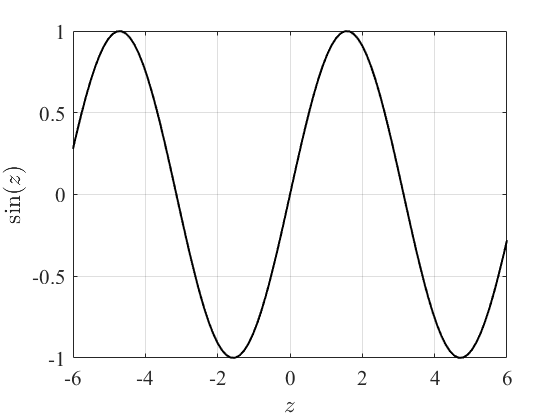
\includegraphics[width=0.35\textwidth]{Pictures/sin.png}
    \end{center}
    \caption[Graph of $\Phi$.]{Graph of $\Phi$ (unconstrained function).}
        \label{fig:sin example 1}
\end{figure}
\begin{figure}[ht!]
    \begin{center}
        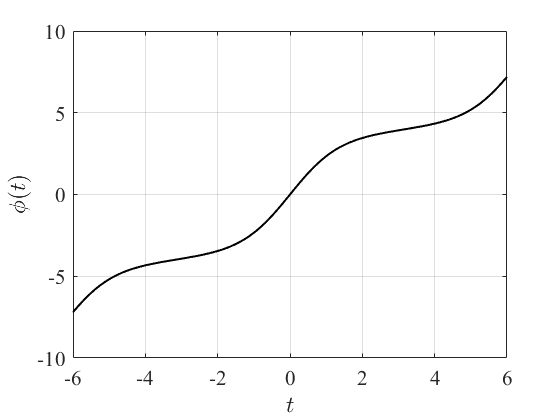
\includegraphics[width=0.35\textwidth]{Pictures/increased_sin.png}
    \end{center}
    \caption[Graph of $\phi = \mathcal{R}_{\mathrm{inc}}\{\Phi\}$.]{Graph of $\phi = \mathcal{R}_{\mathrm{inc}}\{\Phi\}$ (after first rectification).}
        \label{fig:sin example 2}
\end{figure}
\begin{figure}[ht!]
    \begin{center}
    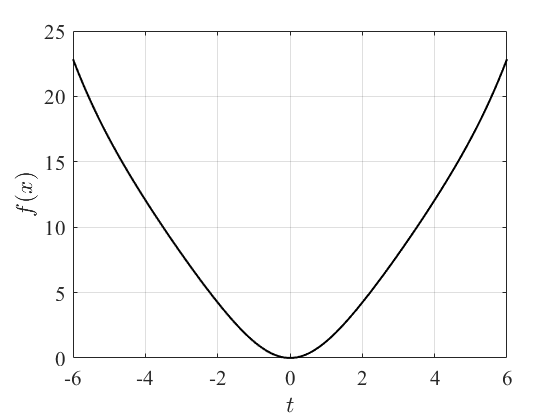
\includegraphics[width=0.35\textwidth]{Pictures/rectified_sin.png}
    \end{center}
    \caption[Graph of $f = \mathcal{R}_{\mathrm{cvx}}\{\phi\} = \mathcal{R}\{\Phi\}$.]{Graph of $f = \mathcal{R}_{\mathrm{cvx}}\{\phi\} = \mathcal{R}\{\Phi\}$ (fully rectified function).}
    \label{fig:sin example 3}
\end{figure}
Notice that in this example, the derivative of the rectified function $f$ cannot be required to vanish at an arbitrary point (as in Eq.~\eqref{eq:constraint-stationarity} for example), since the primary function $\Phi$ is fixed (as opposed to the case where it can be trained). 
\end{remark}


\section{Applications}\label{sec:applications}
We consider a standard setting where data are provided in the form stress-strain responses. For an incompressible material for instance, the Cauchy stress associated with the rectified NN is evaluated as
\begin{equation}
    {\bf\Sigma}^*(\bfF) = 2 {\bfF} \left(\sum_{i = 1}^{3} \frac{\partial w_i^*(I_i)}{ \partial I_i} \frac{\partial I_i}{ \partial \bfC} \right) \bfF^T - p\bfI\,,
\end{equation}
where the left-hand side depends on the parameters of the NN, $w_i^*$ is defined by Eq.~\eqref{eq:def-wistar}, $p$ is a Lagrange multiplier arising from the incompressibility condition (in practice, $p$ is evaluated by imposing a stress-free condition). 

Training with respect to data can be achieved using the cost function
\begin{equation}\label{eq:def-Ld}
     \mathcal{L}_d = \frac{\sum_{i = 1}^{N} \left( \Sigma^*(\bfF(\lambda_i)) - \Sigma^{\textnormal{data}}(\bfF(\lambda_i)) \right)^2}{\sum_{i = 1}^{N} \Sigma^{\textnormal{data}}(\bfF(\lambda_i))^2 }\,,
\end{equation}
along a loading path $\lambda \mapsto \bfF(\lambda)$, discretized with $N$ points. Here, $\Sigma^*$ denotes the relevant stress component (\textit{e.g.}, along testing direction), and $\{(\lambda_i, \Sigma^{\textnormal{data}}(\bfF(\lambda_i)))\}_{i = 1}^{N}$ constitutes the dataset. Note that the above loss function can be readily extended to cases where several loading conditions are considered (see Section \ref{subsec:exp-app}).

In the applications presented below, no attempt was made to fully optimize network architectures and training strategies. The numbers of layers and neurons per layer were determined through a standard parametric analysis on the validation loss defined by Eq.~\eqref{eq:def-Ld}. No activation function was used for the toy problem presented in Section \ref{subsec:toy}, while the sigmoid activation function was selected for all hidden layers in all other examples (in Sections \ref{subsec:MR}, \ref{subsec:anisotropic-app}, and \ref{subsec:exp-app}). 

The Adaptive Moment Estimation (ADAM) algorithm was used for training, with an implementation in JAX \cite{jax2018github}. 

\subsection{Toy Problem}\label{subsec:toy}
We first consider a toy example where the target convex function is given as
\begin{align}
        f^\textnormal{target}(x) = k_1 \exp\left( \frac{(x - k_2)^2}{2k_3^2} \right)\,, \quad \forall x \in \mathbb{R}\,,
\end{align}
where $k_1= 10$, $k_2= 5$, and $k_3= 20$. We seek to construct an approximation over the interval $I = [0, 10]$, centered without loss of generality around the abscissa $x = k_2$ at which $f^\textnormal{target}$ reaches its minimum, with $f(k_2) = k_1$. A set of $100$ equidistant data points is used for fitting, and 20 \% data points are used as the validation set. Adopting the generic notation $\psi$ for the neural network, the rectified model reads as
\begin{equation}
    f(x) = k_1 - \int_{0}^{k_2} \phi(t) \,dt + \int_{0}^x \phi(t) \,dt\,, \quad \forall x \in [0, 10]\,,
\end{equation}
where
\begin{equation}
    \phi(t) = \psi(0) + \int_{0}^t g\left(\frac{d\psi(z)}{dz}\right) \,dz\,.
\end{equation}
Three different choices for $g$ were considered, namely the square function $g(x) = x^2$, the exponential function $g(x) = \exp(x)$, and the modified soft-plus function $g(x) = \log(2^x+1)/\log(2)$. 

In this example, a simple neural network architecture with one hidden layer and two neurons is used (without activation functions). The learning rate for the ADAM optimizer is set to 0.01. Mean square validation errors for the rectified functions are reported in Tab.~\ref{tab:toy-problem-validation-errors} for the three choices of $g$. 
\begin{table}[ht!]
\caption[Results for the validation step (toy problem).]{Results for the validation step: $L^2$-norm errors for the rectified neural network model (toy problem).}
\label{tab:toy-problem-validation-errors}
\begin{center}
    \begin{tabular}{|c|c|} 
        \hline
        Function $g$ & Error $\epsilon$ \\ 
        \hline
        Square & $1.5850 \times 10^{-7}$ \\ 
        \hline
        Exponential & $2.0018 \times 10^{-5}$ \\ 
        \hline
        Soft-plus & $1.6069 \times 10^{-7}$ \\ 
        \hline
        \end{tabular}
\end{center}
\end{table}
The square and modified soft-plus functions provide fairly similar validation errors, smaller than the one obtained with the exponential function. In addition, the model rectified with the square function converged in 3,000 epochs, while the rectified model with the modified soft-plus function converged in about 8,000 epochs. The model with the exponential function converged in more than 10,000 epochs, which is slower than with the other two positive functions. In order to qualitatively assess the accuracy, the predictions obtained with the rectified neural network for the validation dataset are shown in Fig.~\ref{fig:toy-problem-qualitative-results} (see Tab.~\ref{tab:toy-problem-validation-errors} for validation metrics).
\begin{figure}[ht!]
    \begin{center}
        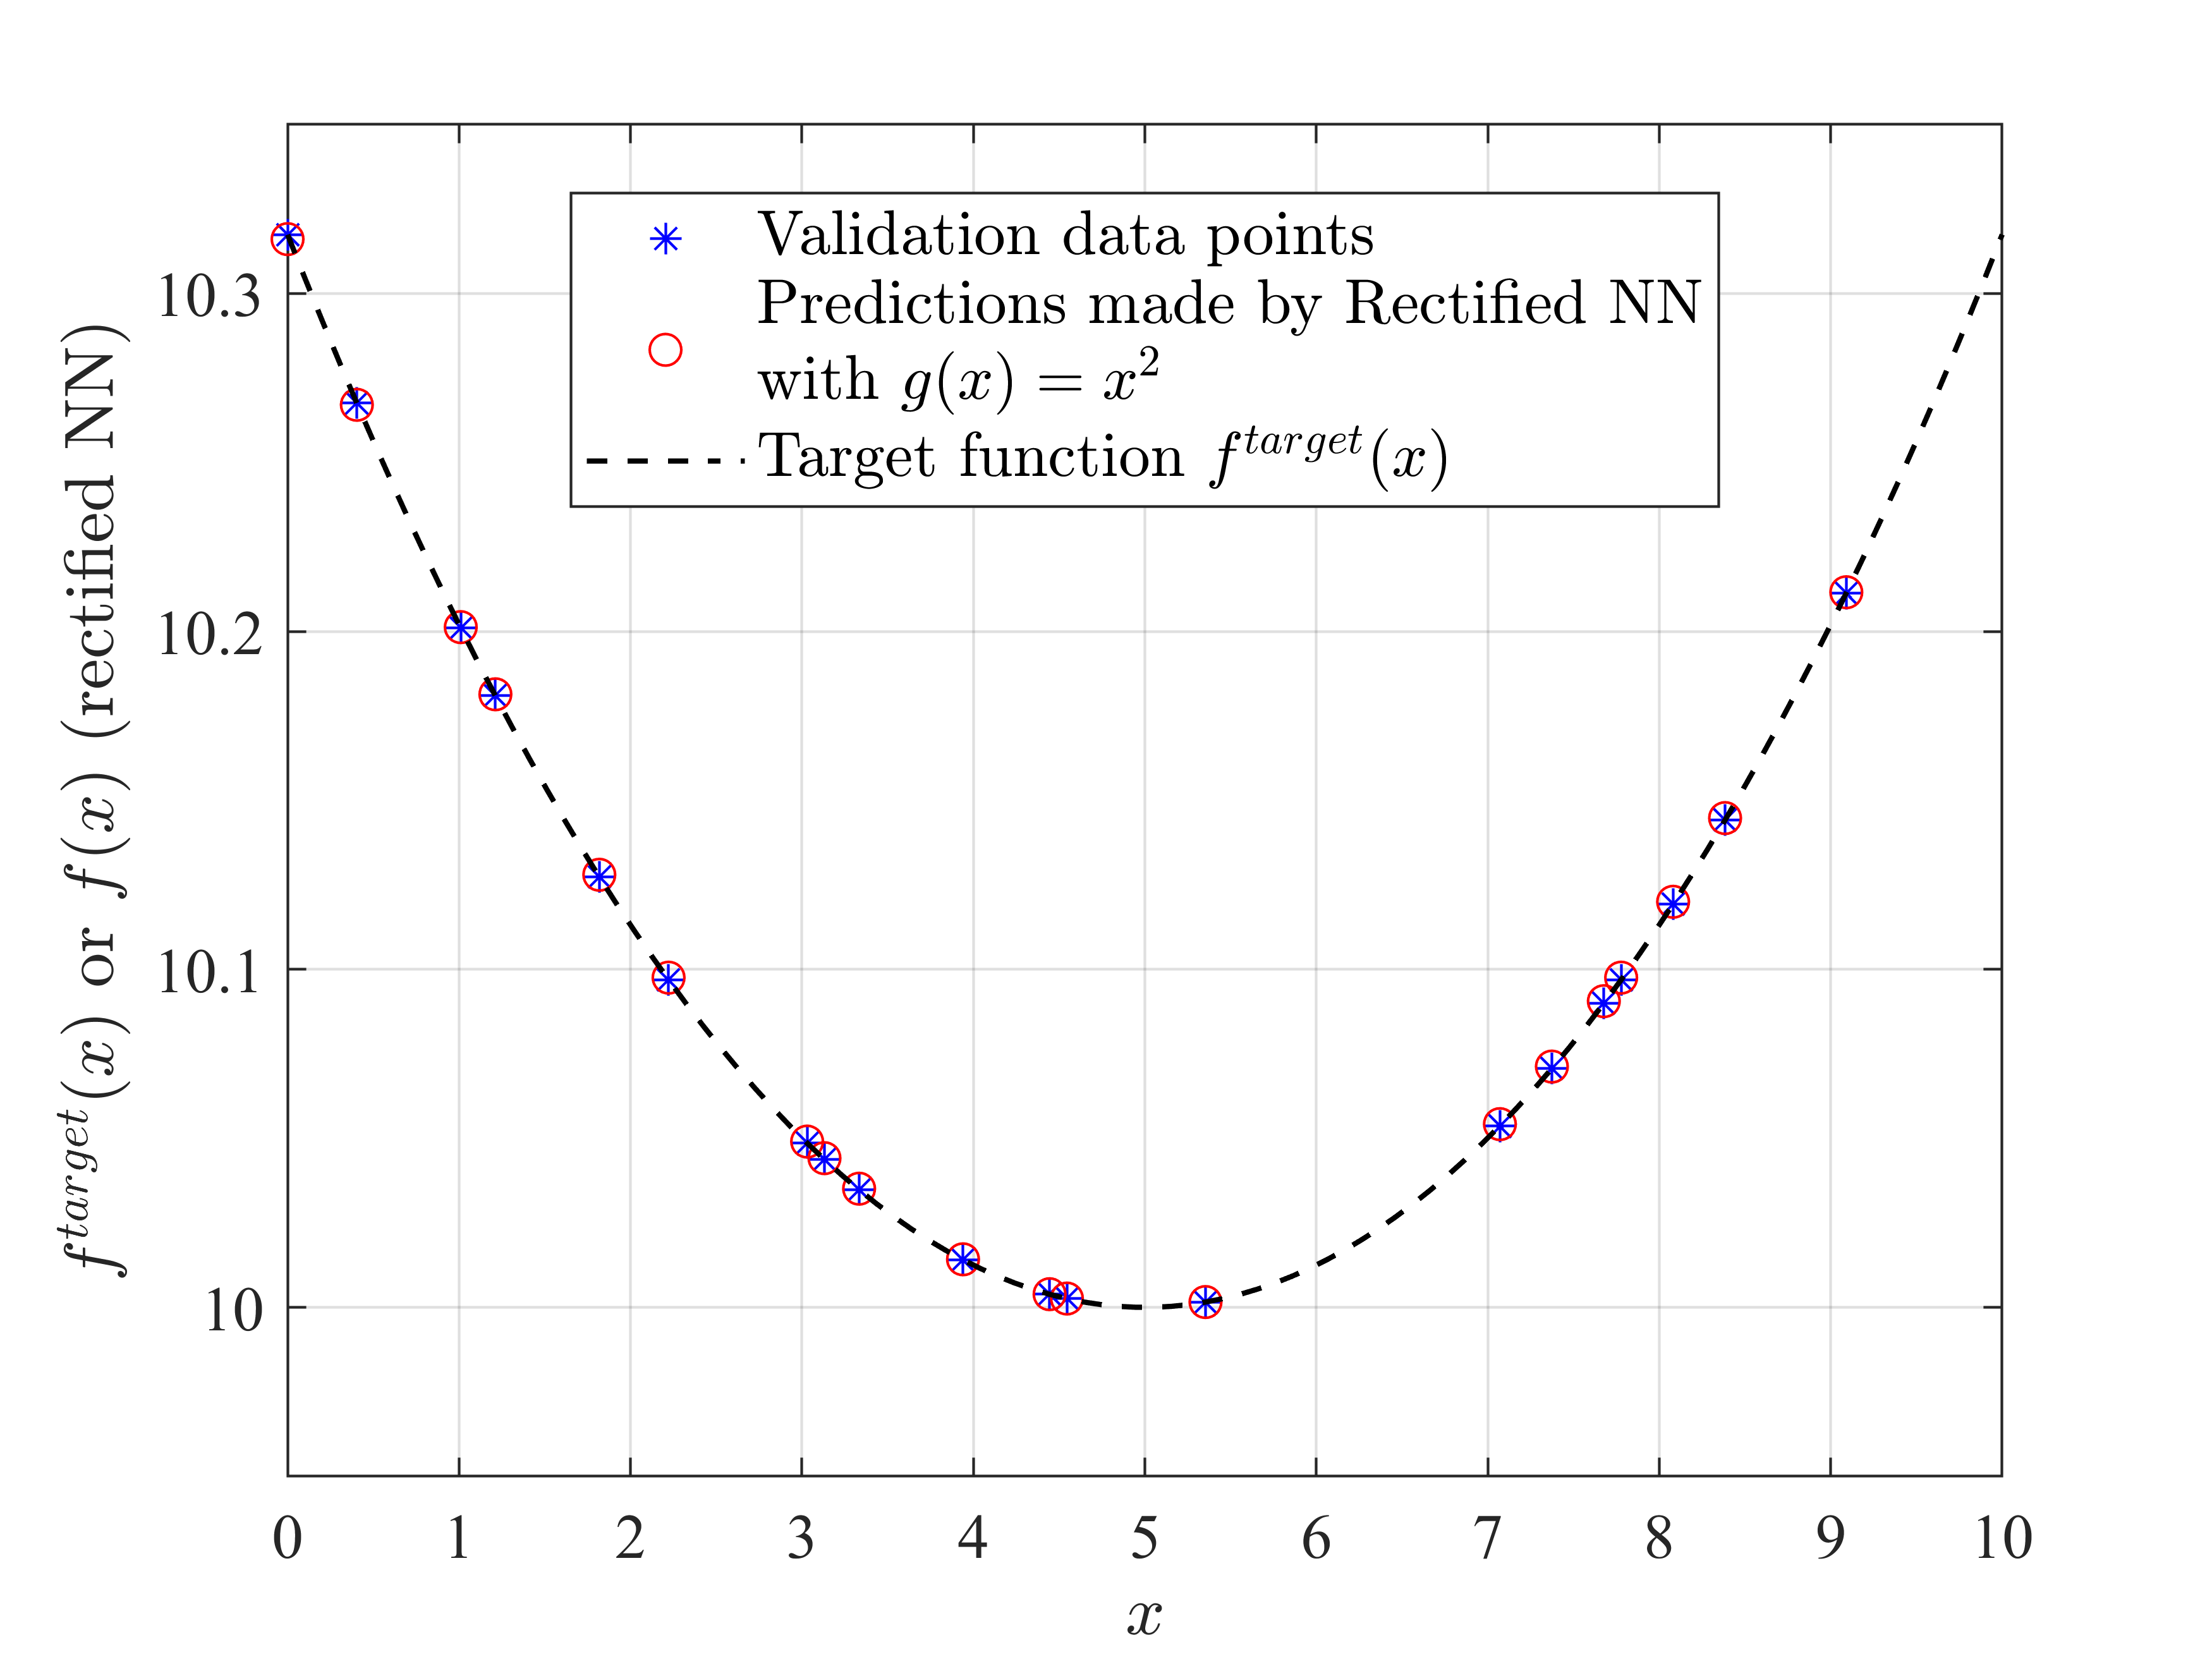
\includegraphics[width = 0.5\textwidth]{Pictures/toy.png}
    \end{center}
    \caption[Target function, reference values, and rectified neural network predictions.]{Target function (black dashed line), reference values (blue star), and rectified neural network predictions (red circles) for the validation dataset (random selection).}
    \label{fig:toy-problem-qualitative-results}
\end{figure}
Recall that no restrictions are imposed on weights and activation functions in the proposed formulation.

\subsection{Mooney-Rivlin Model}\label{subsec:MR}
Here we address the case of a Mooney–Rivlin material, defined by the stored energy function
\begin{equation}
    w{^\textnormal{MR}}(I_1,I_2) = C_1(I_1 - 3) + C_2(I_2 - 3)\,, \label{eq:MR}
\end{equation}
where $C_1$ and $C_2$ are strictly positive material parameters (see \cite{ciarlet1988mathematical}, p.~189). The rectified model is written as
\begin{equation}
    w^*(I_1, I_2) = w_1^*(I_1) + w_2^*(I_2)\,,
\end{equation}
with 
\begin{align}
    w_1^*(I_1) = \mathcal{R}\{\psi_1(\{\bfW_j^{(1)}, \bfb_j^{(1)}\}_{j = 1}^{n_1})\}(I_1)
\end{align}
and
\begin{align}
w_2^*(I_2) = \mathcal{R}\{\psi_2(\{\bfW_j^{(2)}, \bfb_j^{(2)}\}_{j = 1}^{n_2})\}(I_2)\,.
\end{align}
The Cauchy stress is given by (see \cite{HolzapfelBook}, p. 224)
\begin{equation}
    \boldsymbol{\Sigma} = 2C_1\bfB - 2C_2\bfB^{-1} - p \bfI\,.
\end{equation}
We consider uniaxial tension along the first direction for training purposes, in which case the uniaxial Cauchy stress writes 
\begin{equation}
    \Sigma(\lambda) = 2\left(C_1 + \frac{ C_2}{\lambda}\right)\left(\lambda^2 - \frac{1}{\lambda}\right)\,, \label{eq:MR_Cauchy}
\end{equation}
where $\lambda$ is the driving principal stretch. The uniaxial Cauchy stress associated with the rectified model can be evaluated as
\begin{equation}
    \Sigma^*(\lambda) = 2 \left( \frac{\partial w_1^*(I_1)}{\partial I_1} + \frac{\partial w_2^*(I_2)}{\partial I_2} \frac{1}{\lambda} \right) \left( \lambda^2 - \frac{1}{\lambda} \right)\,, 
\end{equation}
with
\begin{equation}
    \frac{\partial w_i^*(I_i)}{\partial I_i} =  \left( \psi_i(0) + \int_0^{I_i} g\left(\frac{d\psi_i}{dz}\right)\, dz \right)\,.
\end{equation}
Derivatives are computed using automatic differentiation. In this example, we consider an approximation for $\lambda \in [1.0, 1.4]$ ($I_1 \geq 3$ and $I_2 \geq 3$). The material parameters are arbitrarily chosen as $C_1 = 10$ and $C_2 = 5$. Normalization condition is imposed by taking $w_1^*(3) = w_2^*(3) = 0$ with the constant terms (see Eq.~\eqref{eq:Rec-Con}, with $a = 3$) set to 0. Note that the stress free condition is automatically satisfied owing to the definition of $p$.

Two hundreds datapoints are generated using Eq.~\eqref{eq:MR_Cauchy}, with 20 \% of samples allocated for validation.  Parametric studies on validation error were conducted to identify the NN architecture, using a learning rate set to $0.01$, 5,000 epochs, and the square function (in the first rectifier); see Fig.~\ref{fig:Mr_Err_Study}.
\begin{figure}[ht!]
    \begin{center}
        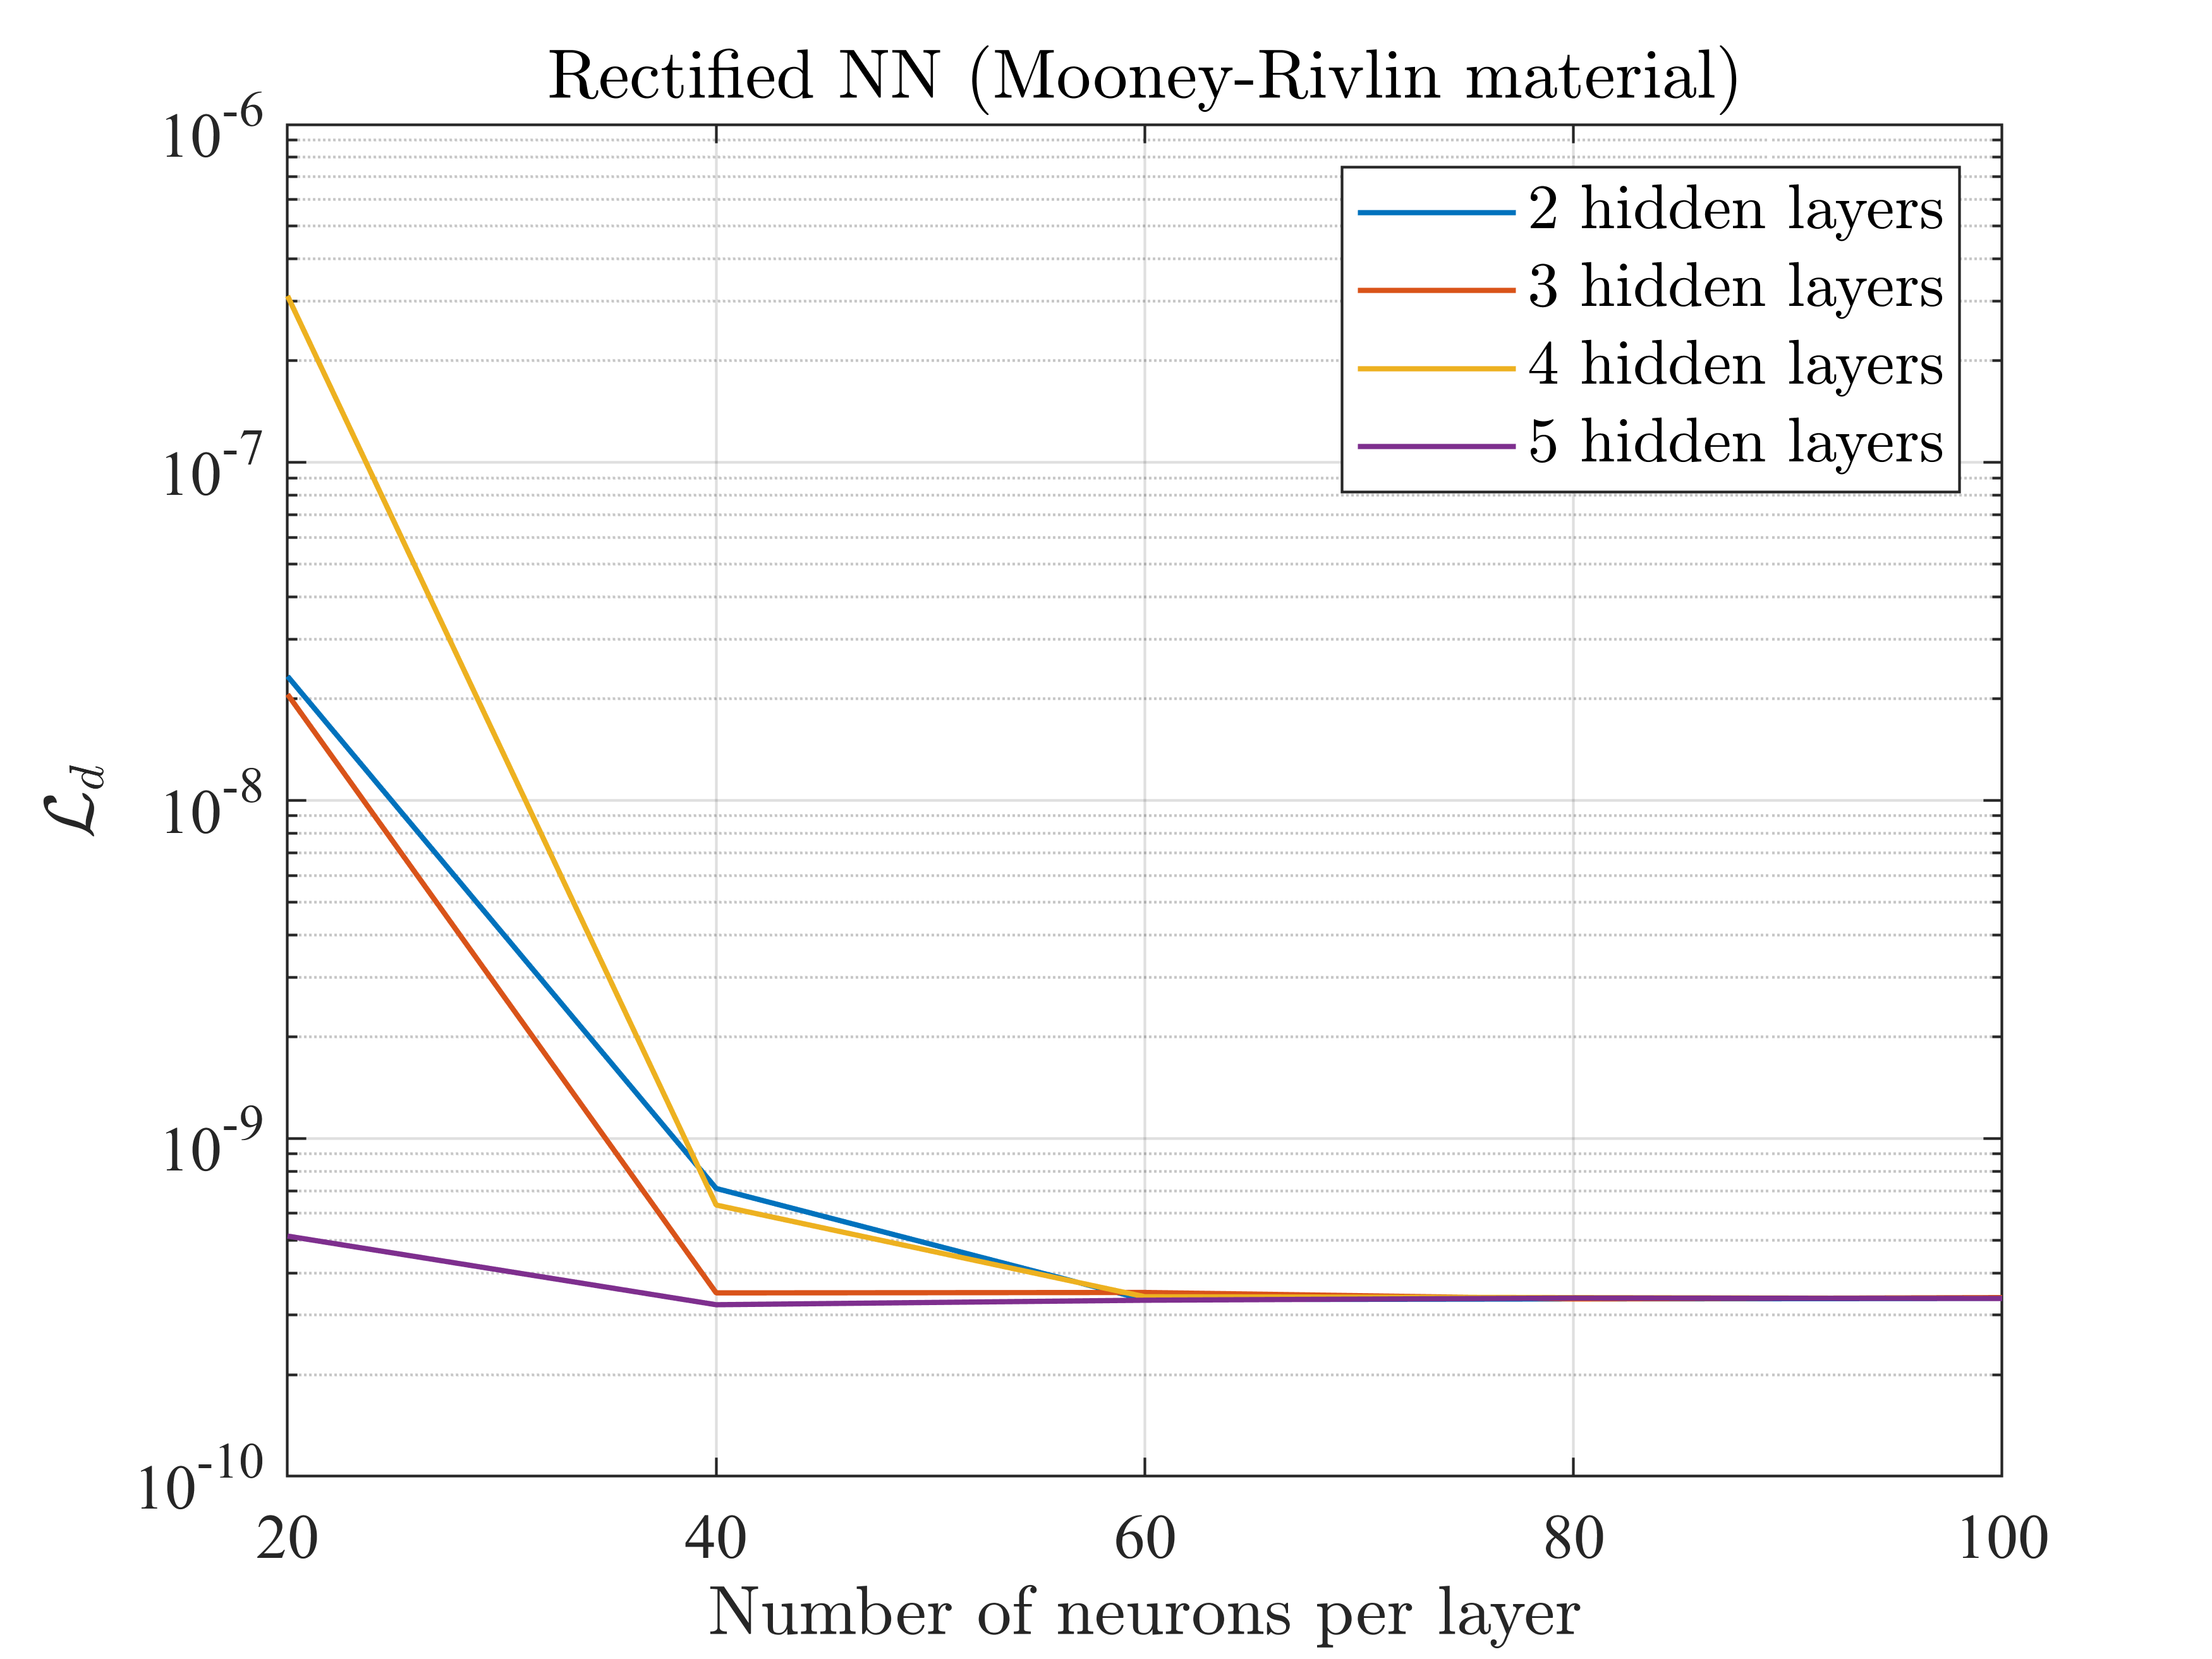
\includegraphics[width = 0.5\textwidth]{Pictures/Mr_Err.png}
    \end{center}
    \caption[Loss $\mathcal{L}_d$ for different neural network architectures.]{Loss $\mathcal{L}_d$ for different neural network architectures on the validation dataset (Mooney-Rivlin material).}
    \label{fig:Mr_Err_Study} 
\end{figure}
Results predicted by the calibrated rectified neural network model (with 5 layers and 40 neurons per layer) on the validation dataset is shown in Fig.~\ref{fig:MR best result 1}.
\begin{figure}[ht!]
    \begin{center}
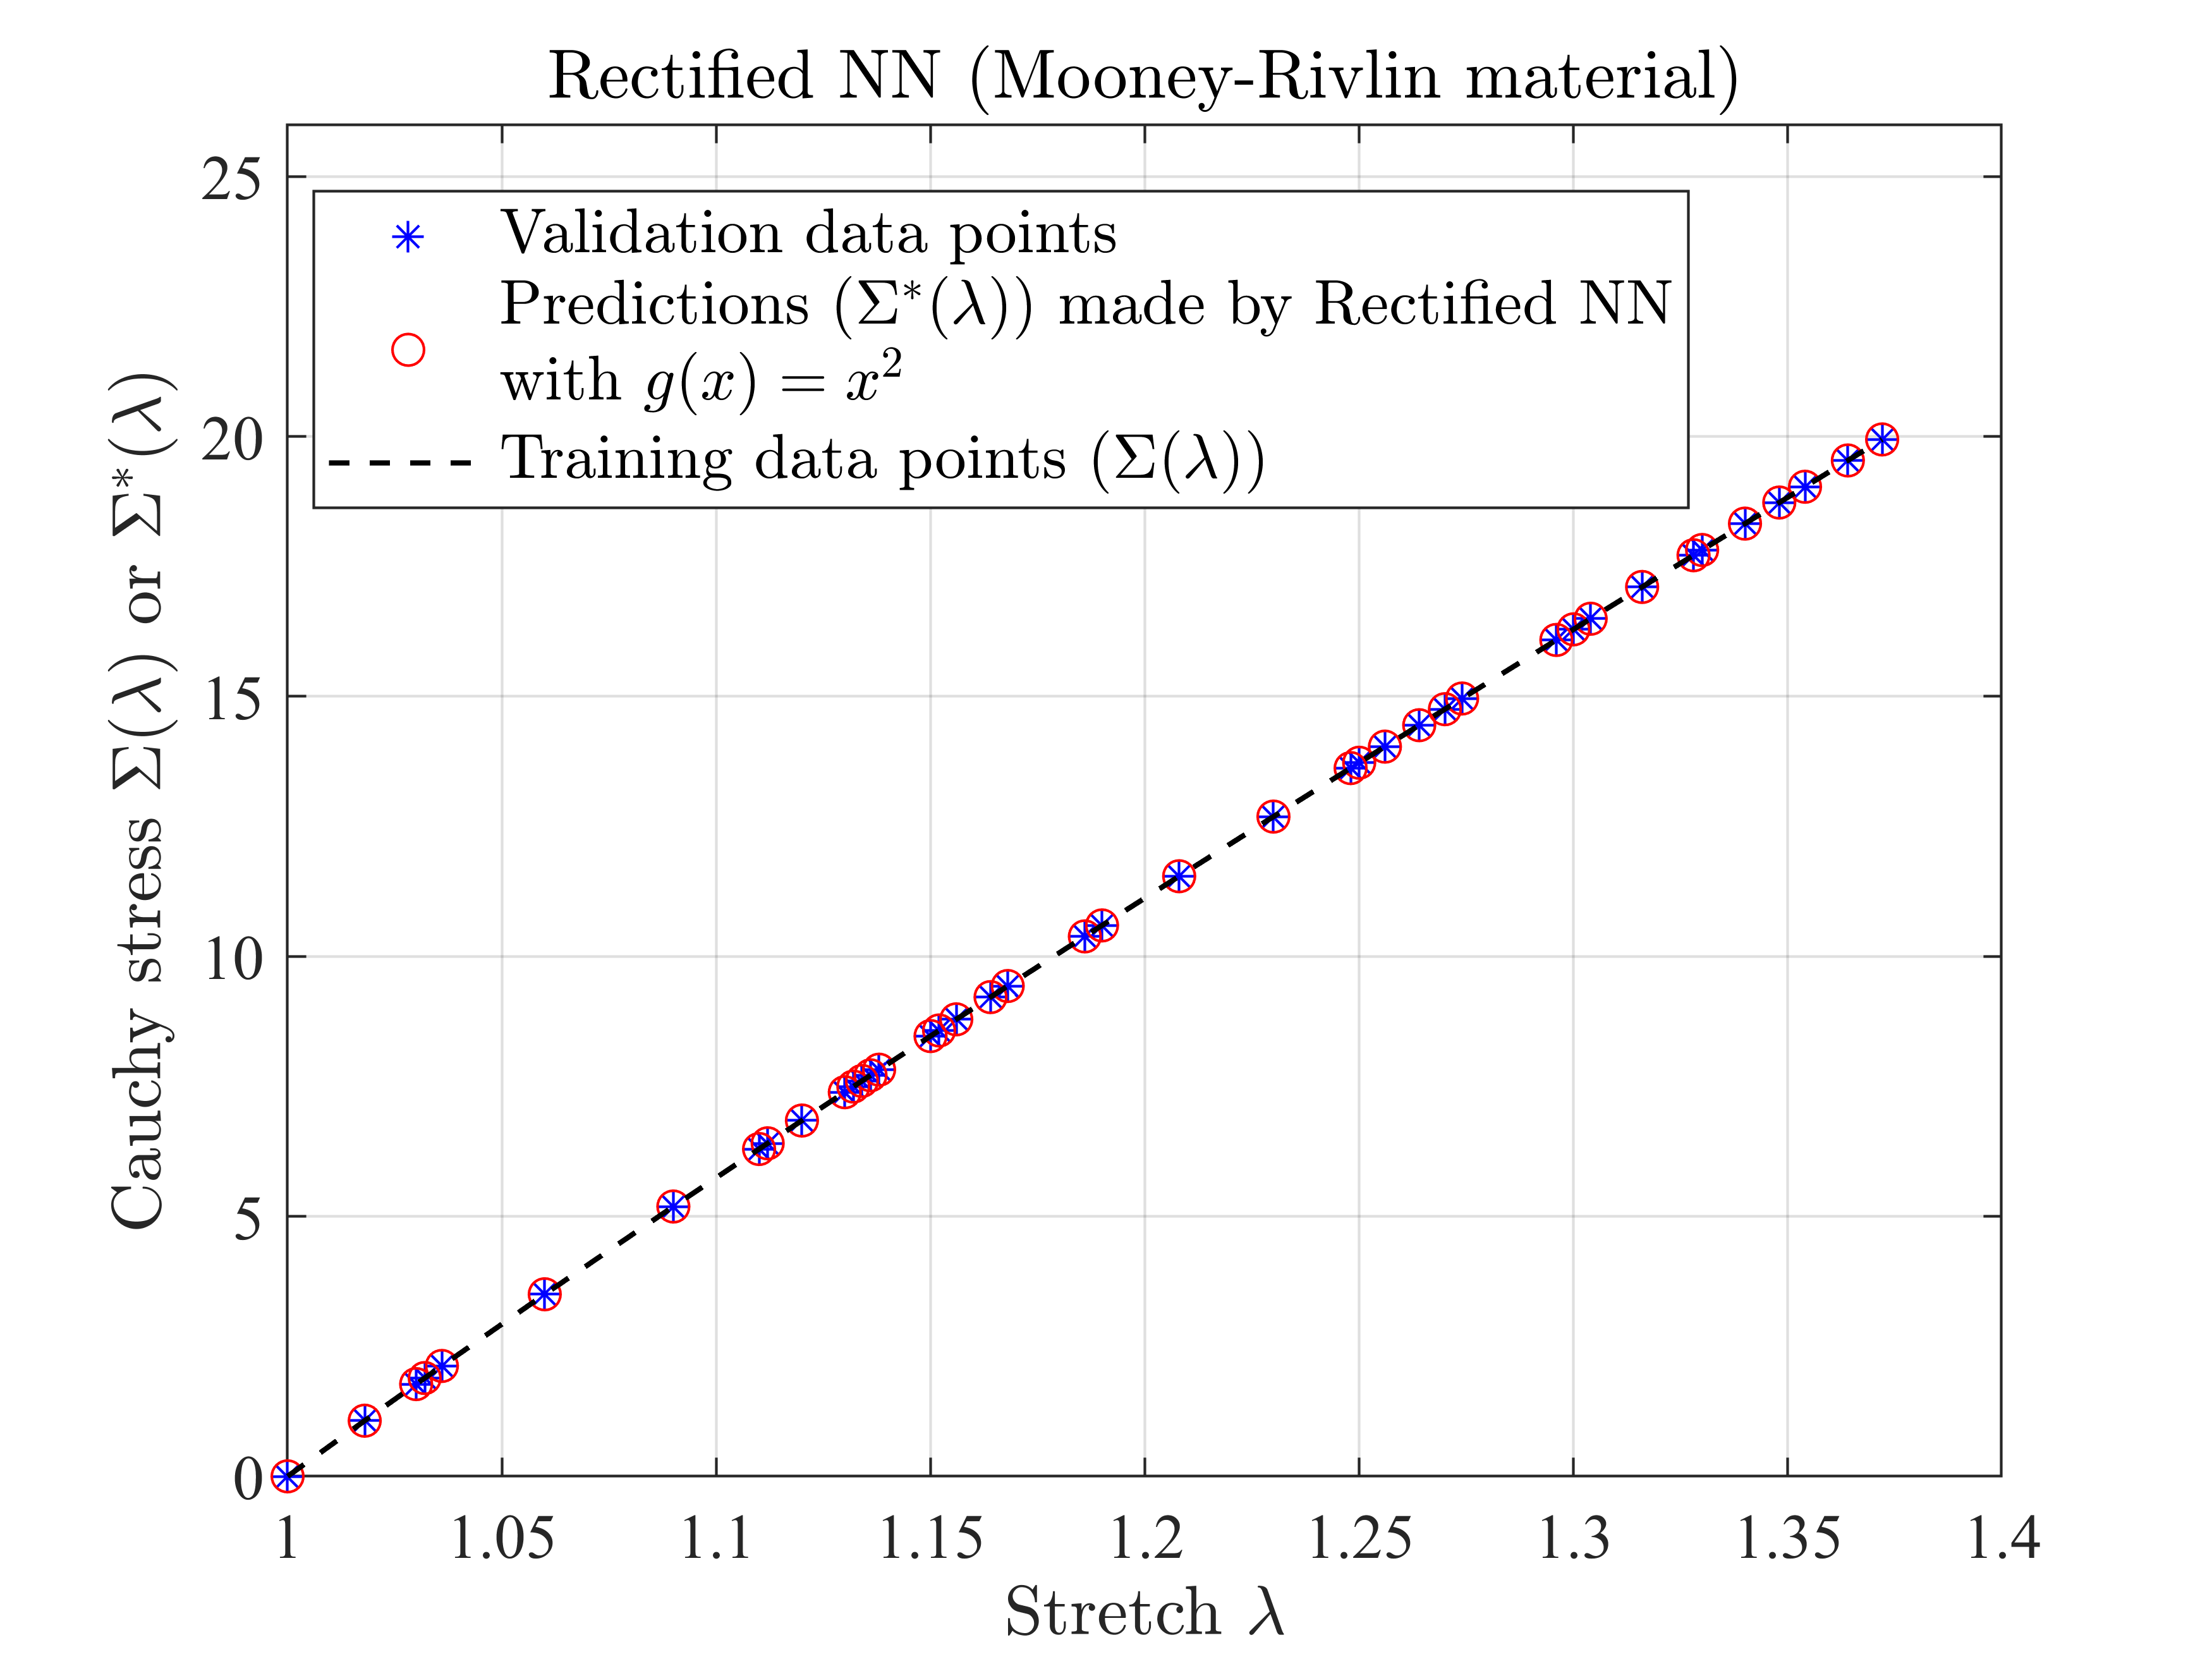
\includegraphics[width=0.5\textwidth]{Pictures/sigma_MR.png}
    \end{center}
    \caption[Reference stress response and values, rectified NN predictions.]{Reference stress response $\lambda \mapsto \Sigma(\lambda)$ (black dashed line), reference values (blue star), and rectified neural network predictions (red circle) for the validation dataset (random selection). Here, 5 hidden layers and 40 neurons per layer are used.}
    \label{fig:MR best result 1}
\end{figure}

\begin{remark} As indicated before, Input-Convex Neural Networks (ICNNs) can be obtained by forcing all weights, except those connected to the input, to be non-negative, and by using only convex non-decreasing activation functions \cite{amos2017input, as2022mechanics,Asad-IJNME,KLEIN2022104703}. In order to evaluate the performance of such constrained neural networks in terms of training results, we consider a model of the form 
\begin{align}
    \psi_{\mathrm{ICNN}}(I_1, I_2) &= \psi_{\mathrm{ICNN}}^{(1)}(I_1) + \psi_{\mathrm{ICNN}}^{(2)}(I_2)\,,
\end{align}
where each ICNN involves unconstrained weights that are mapped to positive weights in the loss function, using the modified soft-plus activation function proposed in \cite{as2022mechanics,Asad-IJNME}. The validation loss history for each approach is shown in Fig.\ref{fig:ERR_history} for the Mooney-Rivlin dataset.
\begin{figure}[ht!]
    \begin{center}
        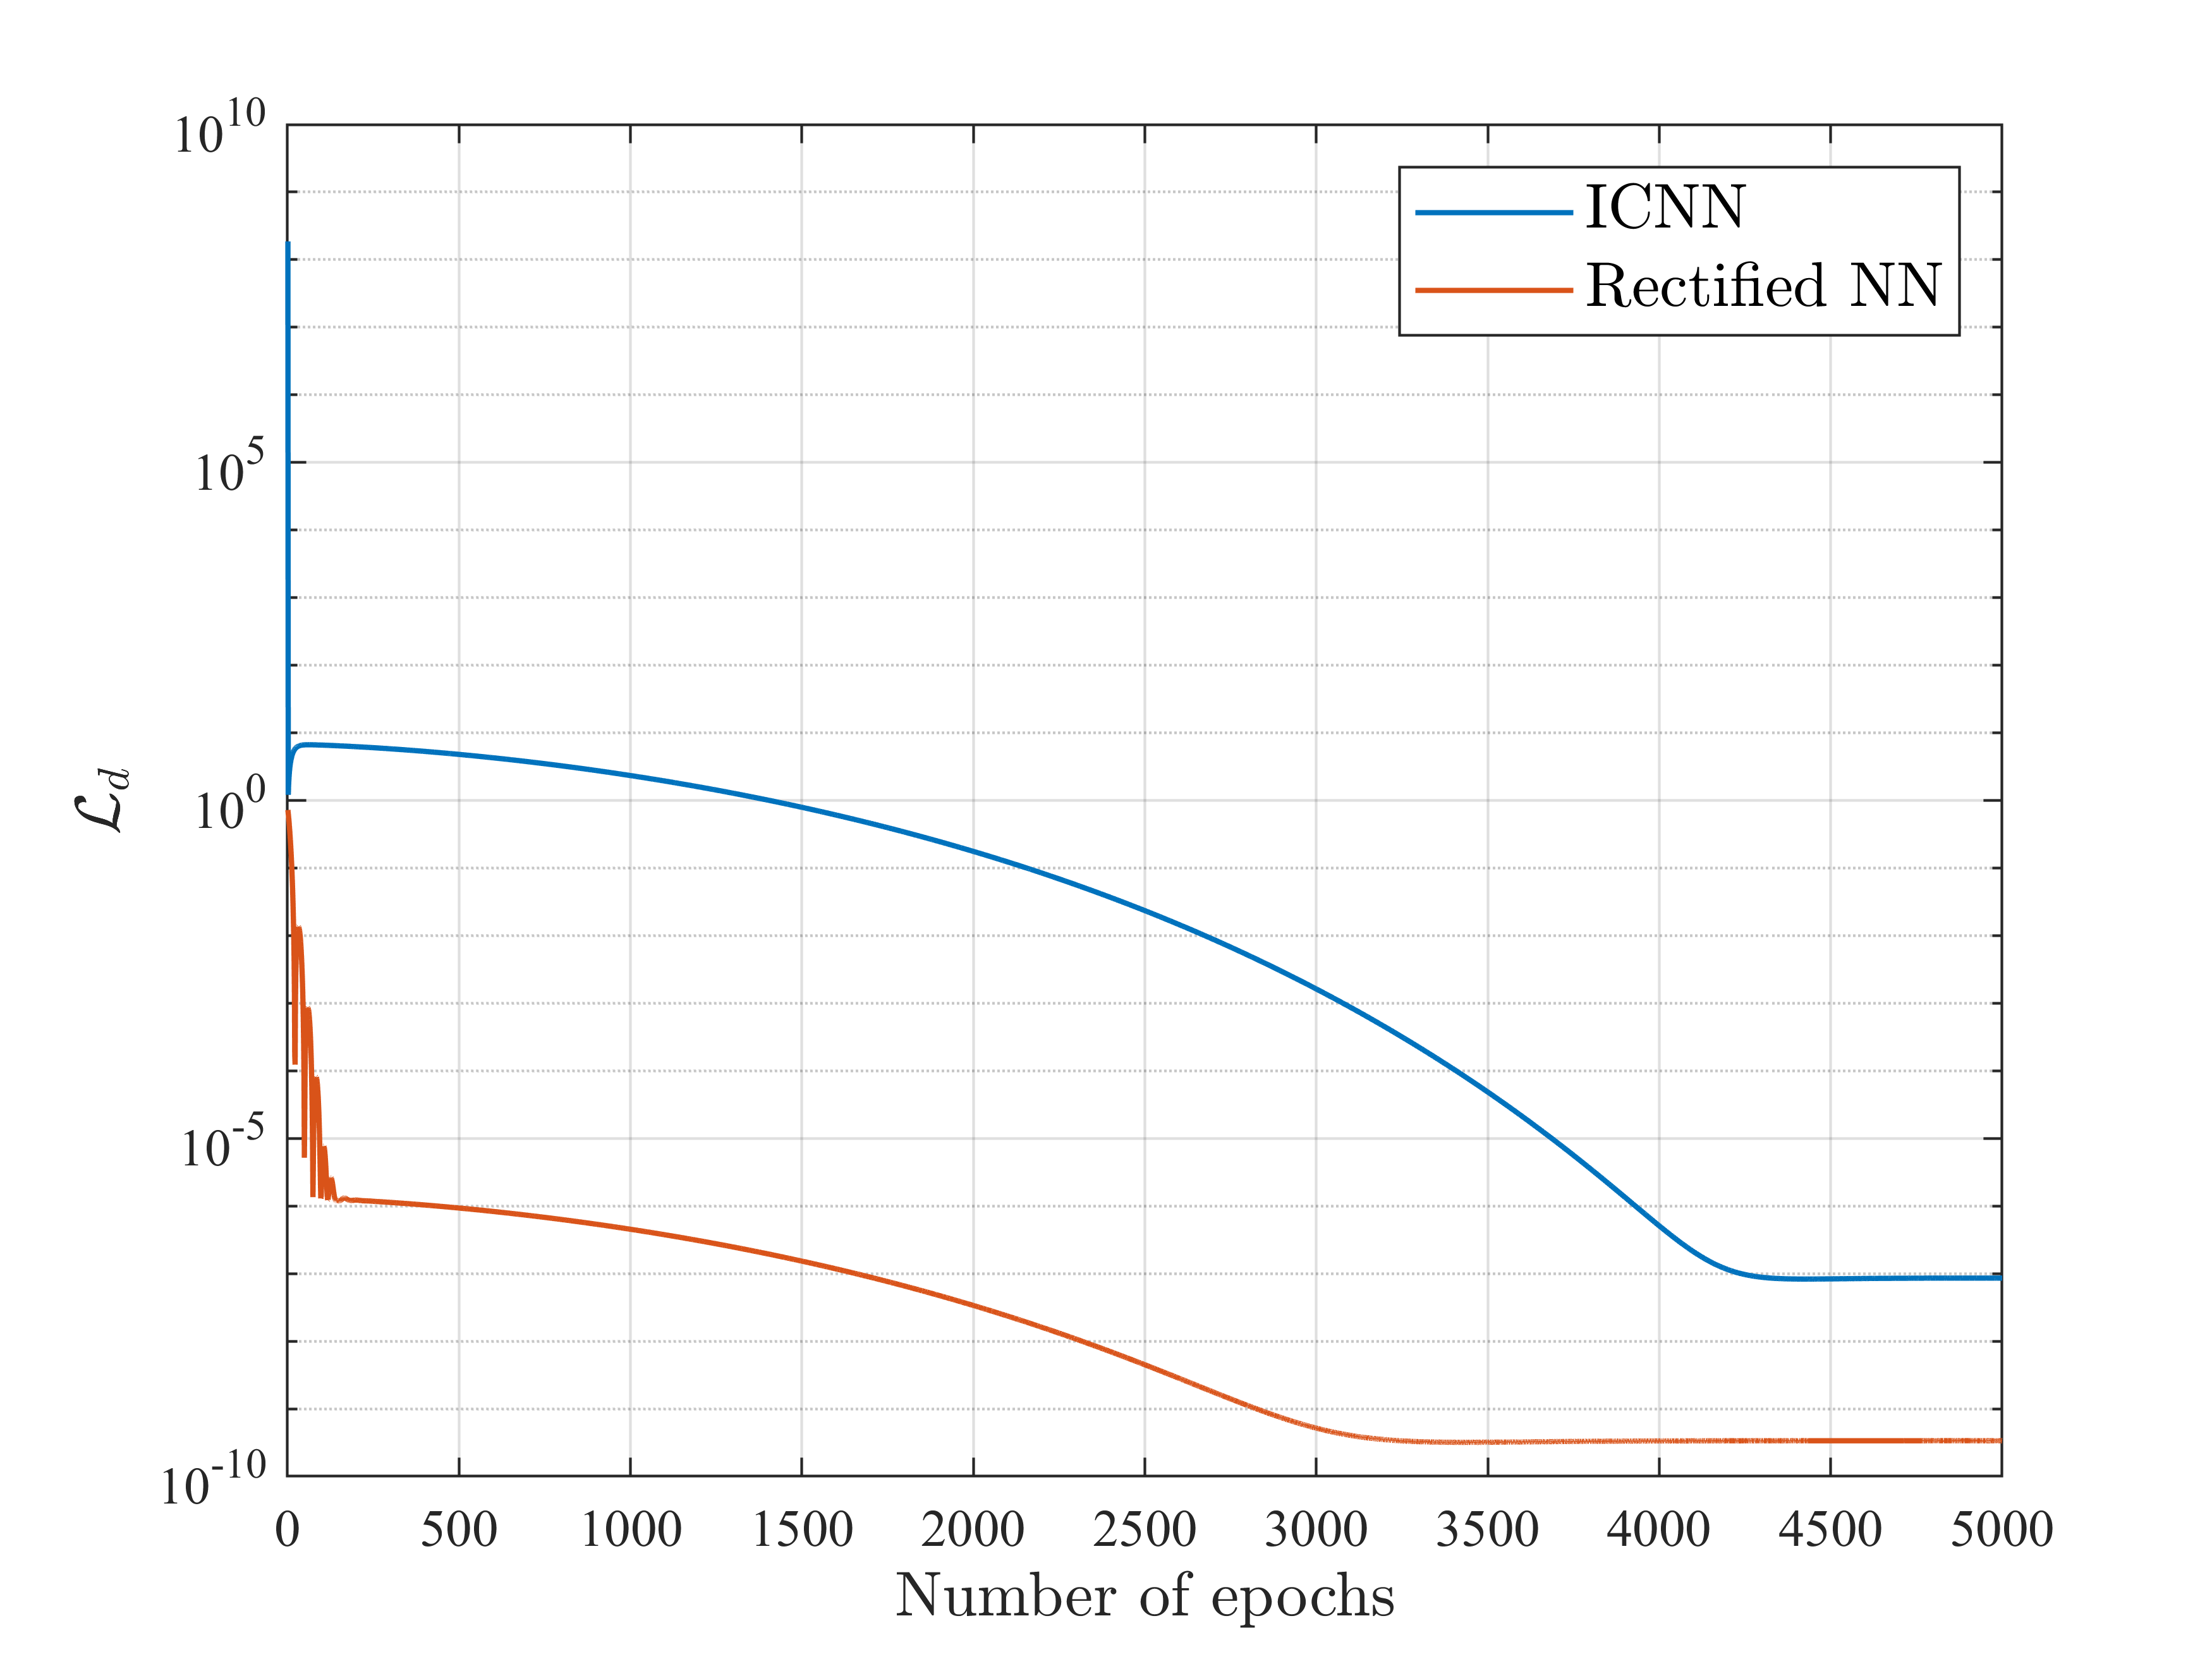
\includegraphics[width = 0.5\textwidth]{Pictures/loss_hist.png}
    \end{center}
    \caption[Loss history for ICNN and the proposed rectified NN.]{Loss history for ICNN and the proposed rectified NN.}
    \label{fig:ERR_history} 
\end{figure}
Reported results were obtained with 2 hidden layers and 20 neurons per layer for both strategies, based on a parametric convergence study on the validation metric. It is seen that the rectified NN converges much faster than the ICNN and leads to a lower training error. While similar results were obtained for a wide range of architectures, it should be pointed out that the computational cost per iteration is greater in the case of rectified NNs, which require numerical integration to be performed. In addition, opposite trends with respect to learning rates were observed: ICNNs tend to perform slightly better at large learning rates (\textit{e.g.}, 1.5) but require a very large number of iterations (greater than 40,000) at standard learning rates (\textit{e.g.}, 0.001). These observations are most likely imputable to the transformation of negative weights, which generates large regions with ``flat'' gradients in the optimization process. In contrast, rectified NNs were found to perform steadily in terms of training cost, regardless of the learning rate, and typically performs (much) better at smaller rates. An extensive comparison of the tradeoffs between these approaches is left for future work.
\end{remark}

\subsection{Anisotropic Model for Digital Dataset} \label{subsec:anisotropic-app}
We next consider an anisotropic strain energy density function, relevant to the modeling of soft biological tissues such as arterial vessels \cite{balzani2006polyconvex,staber2018stochastic}. It should be noticed such materials are often modeled as nearly-incompressible in a computational setting, in which case the strain energy density function is typically expressed in terms of isochoric invariants. The reference function is defined as
\begin{equation}
    w(I_1, I_2, J_4^{(1)}, J_4^{(2)}) = w{^\textnormal{MR}}(I_1,I_2) + w{^\textnormal{A}}(J_4^{(1)}, J_4^{(2)})\,,
\end{equation}
where $w{^\textnormal{MR}}$ is given by Eq.~\eqref{eq:MR} and the anisotropic term is defined as
\begin{equation}
    w{^\textnormal{A}}(J_4^{(1)}, J_4^{(2)}) = \sum_{k=1}^2 w^{\text{ti}} (J_4^{(k)})\,,
\end{equation}
with
\begin{align}
    w^{\text{ti}} (J_4^{(k)}) = \frac{\mu_4}{\beta_4} \left\{ \exp \left(\beta_4 w^B(I_1, J_4^{(k)}) \right) - 1\right\} \label{eq: psi tissue}
\end{align}
where $w^B(I_1, J_4^{(k)}) = (1-\rho)(I_1 - 3)^2 + \rho \langle J_4^{(k)} - 1 \rangle_m^2$, and $J_4^{(k)}= \tr(\bfC \bfM^{(k)})$. The structural tensors $\bfM^{(k)} = \bfa^{(k)} \otimes \bfa^{(k)}$ are defined in terms of the unit vectors 
\begin{subequations}
    \begin{align}
        \bfa^{(1)} &= \cos(\alpha) \bfe^{(1)} + \sin(\alpha)\bfe^{(2)}\,, \\ 
        \bfa^{(2)} &= \cos(\alpha) \bfe^{(1)} - \sin(\alpha)\bfe^{(2)}\,,
    \end{align}
\end{subequations}
where $\bfe^{(1)}$ and $\bfe^{(2)}$ are unit basis vectors and $\alpha$ is the angle defining the directions of anisotropy. In Eq.~\eqref{eq: psi tissue}, $\mu_4$, $\beta_4$, and $\rho$ are material parameters, and $\langle \cdot \rangle_m$ denotes the Macaulay bracket. Note that the angle $\alpha$ is also considered as a trainable parameter.

The rectified neural network is sought as
\begin{equation}\label{eq:rec-model-anisotropic-case}
    w_1^*(I_1) + w_2^*(I_2) + w_3^*(J_4^{(1)}) + w_4^*(J_4^{(2)})\,,
\end{equation}
where
\begin{equation}
    w_i^*(I_i) = \mathcal{R}\{\psi_i(\{\bfW_j^{(i)}, \bfb_j^{(i)}\}_{j = 1}^{n_i})\}(I_i)\,,\quad i=1,2\,,
\end{equation}
\begin{align}
    w_{3}^*(J_4^{(1)}) = \mathcal{R}\{\psi_3(\{\bfW_j^{(3)}, \bfb_j^{(3)}\}_{j = 1}^{n_3})\}(J_4^{(1)})\,,
\end{align}
and
\begin{align}
    w_{4}^*(J_4^{(2)}) = \mathcal{R}\{\psi_4(\{\bfW_j^{(4)}, \bfb_j^{(4)}\}_{j = 1}^{n_4})\}(J_4^{(2)})\,.
\end{align}
Biaxial tension is used for training purposes. The Cauchy stress associated with the reference model is obtained as
\begin{align}
     \Sigma(\lambda) = \Sigma^{\text{MR}}(\lambda) + \Sigma_{(1)}^{\text{ti}} (\lambda) + \Sigma_{(2)}^{\text{ti}} (\lambda)\,,
\end{align}
with
\begin{equation}
    \Sigma^{\text{MR}}(\lambda) = 2C_1(\lambda^2 - \frac{1}{\lambda^4}) - 2C_2(\frac{1}{\lambda^2} - \lambda^4)\,,
\end{equation}
and
\begin{align}
    \Sigma^{\text{ti}}_{(k)}(\lambda) = & \, 4 \lambda^2 \mu_4 \left\{ (1-\rho)(I_1 - 3)\left(1 - \frac{1}{\lambda^6}\right) \right.  \nonumber \\
    & \quad + \left. \rho \langle J_4^{(k)} - 1 \rangle_m \cos^2(\alpha) \right\}  \nonumber\\
    &\quad \times \exp(\beta_4 w^B(I_1, J_4^{(k)}))\,, \quad k = 1,2\,.
\end{align}
with a slight abuse of notation. The Cauchy stress for the rectified model defined by Eq.~\eqref{eq:rec-model-anisotropic-case} is given by
\begin{align}\label{eq:ANI_Cauchy}
    \Sigma^{*} = \Sigma^*_1(\lambda) + \Sigma^*_2(\lambda) +  \Sigma^*_3(\lambda) + \Sigma^*_4(\lambda)\,,
\end{align}
where terms in the right-hand side are defined as $\Sigma^*_1(\lambda) = 2 \frac{\partial w_1^*(I_1)}{\partial I_1} \left( \lambda^2 - \frac{1}{\lambda^4} \right)$, 
\begin{equation}
    \Sigma^*_1(\lambda) = 2 \frac{\partial w_1^*(I_1)}{\partial I_1} \left( \lambda^2 - \frac{1}{\lambda^4} \right)\,, 
\end{equation}
\begin{equation}
    \Sigma^*_2(\lambda) = -2 \frac{\partial w_2^*(I_2)}{\partial I_2} \left(\frac{1}{\lambda^2} - \lambda^4 \right)\,,
\end{equation}
\begin{equation}
    \Sigma_3^*(\lambda) = 2 \lambda^2 \frac{\partial w_3^*(J_4^{(1)})}{\partial J_4^{(1)}} \cos^2(\alpha)\,,
\end{equation}
\begin{equation}\label{eq:aniso-last-stress-component}
    \Sigma_4^*(\lambda) = 2 \lambda^2 \frac{\partial w_4^*(J_4^{(2)})}{\partial J_4^{(2)}} \cos^2(\alpha)\,.
\end{equation}
Since $\cos(\alpha) \neq 0$ in practice, the stress free constraint reduces to $\Sigma^*_3(1) + \Sigma^*_4(1) = 0$.
% \begin{align}\label{eq:stress-free-constraint-anisotropic-model}
%     \Sigma^*_3(1) + \Sigma^*_4(1) = 0\,.
% \end{align}
In the numerical example below, the material parameters correspond to the values identified in \cite{CHEN2022114897} for sample \#10 in the media layer: $C_1 = 0.7071$ [kPa], $C_2 = 0.0531$ [kPa], $\alpha = 0.2740$ [rad], $\mu_4 = 15.5753$ [kPa], $\beta_4 = 2.5561$, and $\rho = 0.0986$. Similarly to the previous case, we generated 200 datapoints, 20\% of which are used as the validation set. The learning rate is set to 0.005 for the first 3,000 epochs and then to 0.001 for 3,000 epochs, and presented results were obtained using the exponential function in the rectifier (i.e., $g(x) = \exp(x)$). The validation errors for different neural network architectures are shown in Fig.~\ref{fig:ani_err}.
\begin{figure}[ht!]
    \begin{center}
    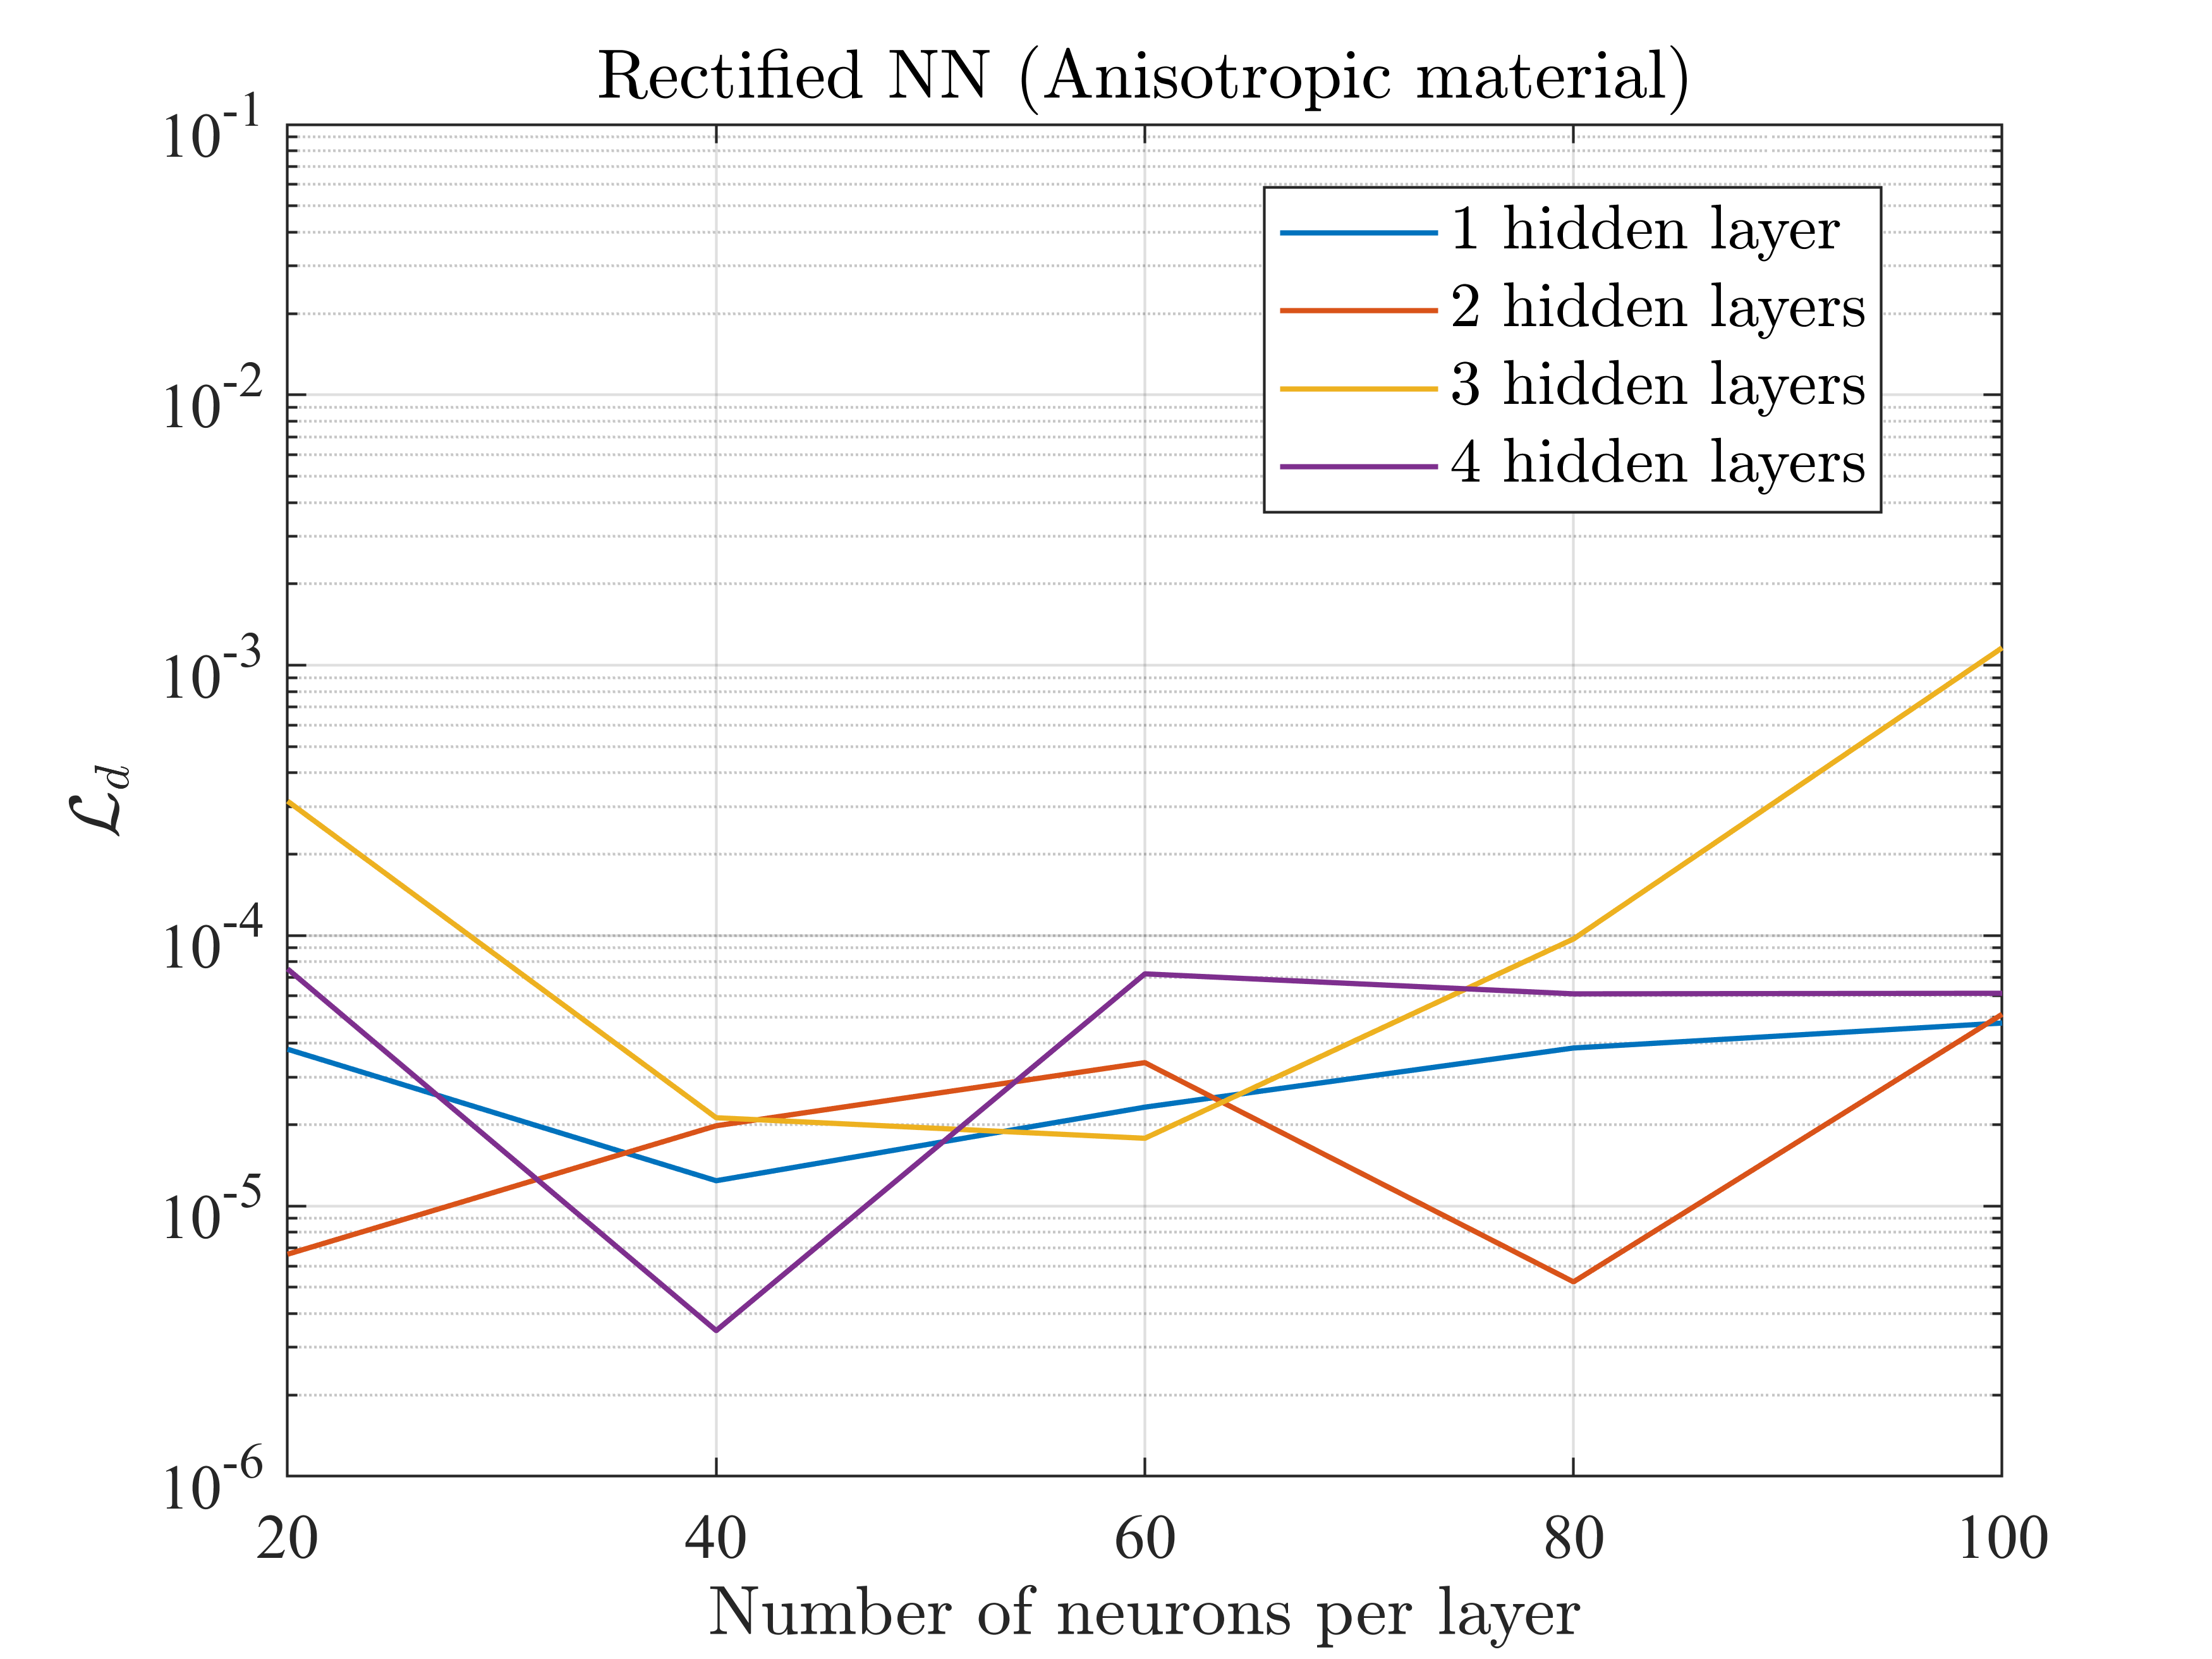
\includegraphics[width=0.5\textwidth]{Pictures/ANI_ERR.png}
    \end{center}
    \caption[Parametric study for RNN architectures.]{Parametric study of the mean squared error for different NN architectures on the validation dataset (Anisotropic material).}
    \label{fig:ani_err}
\end{figure}
Results predicted with the fitted rectified neural network model on the validation dataset are shown in Figs.~\ref{fig:ANI best result 1}.
\begin{figure}[ht!]
    \begin{center}
        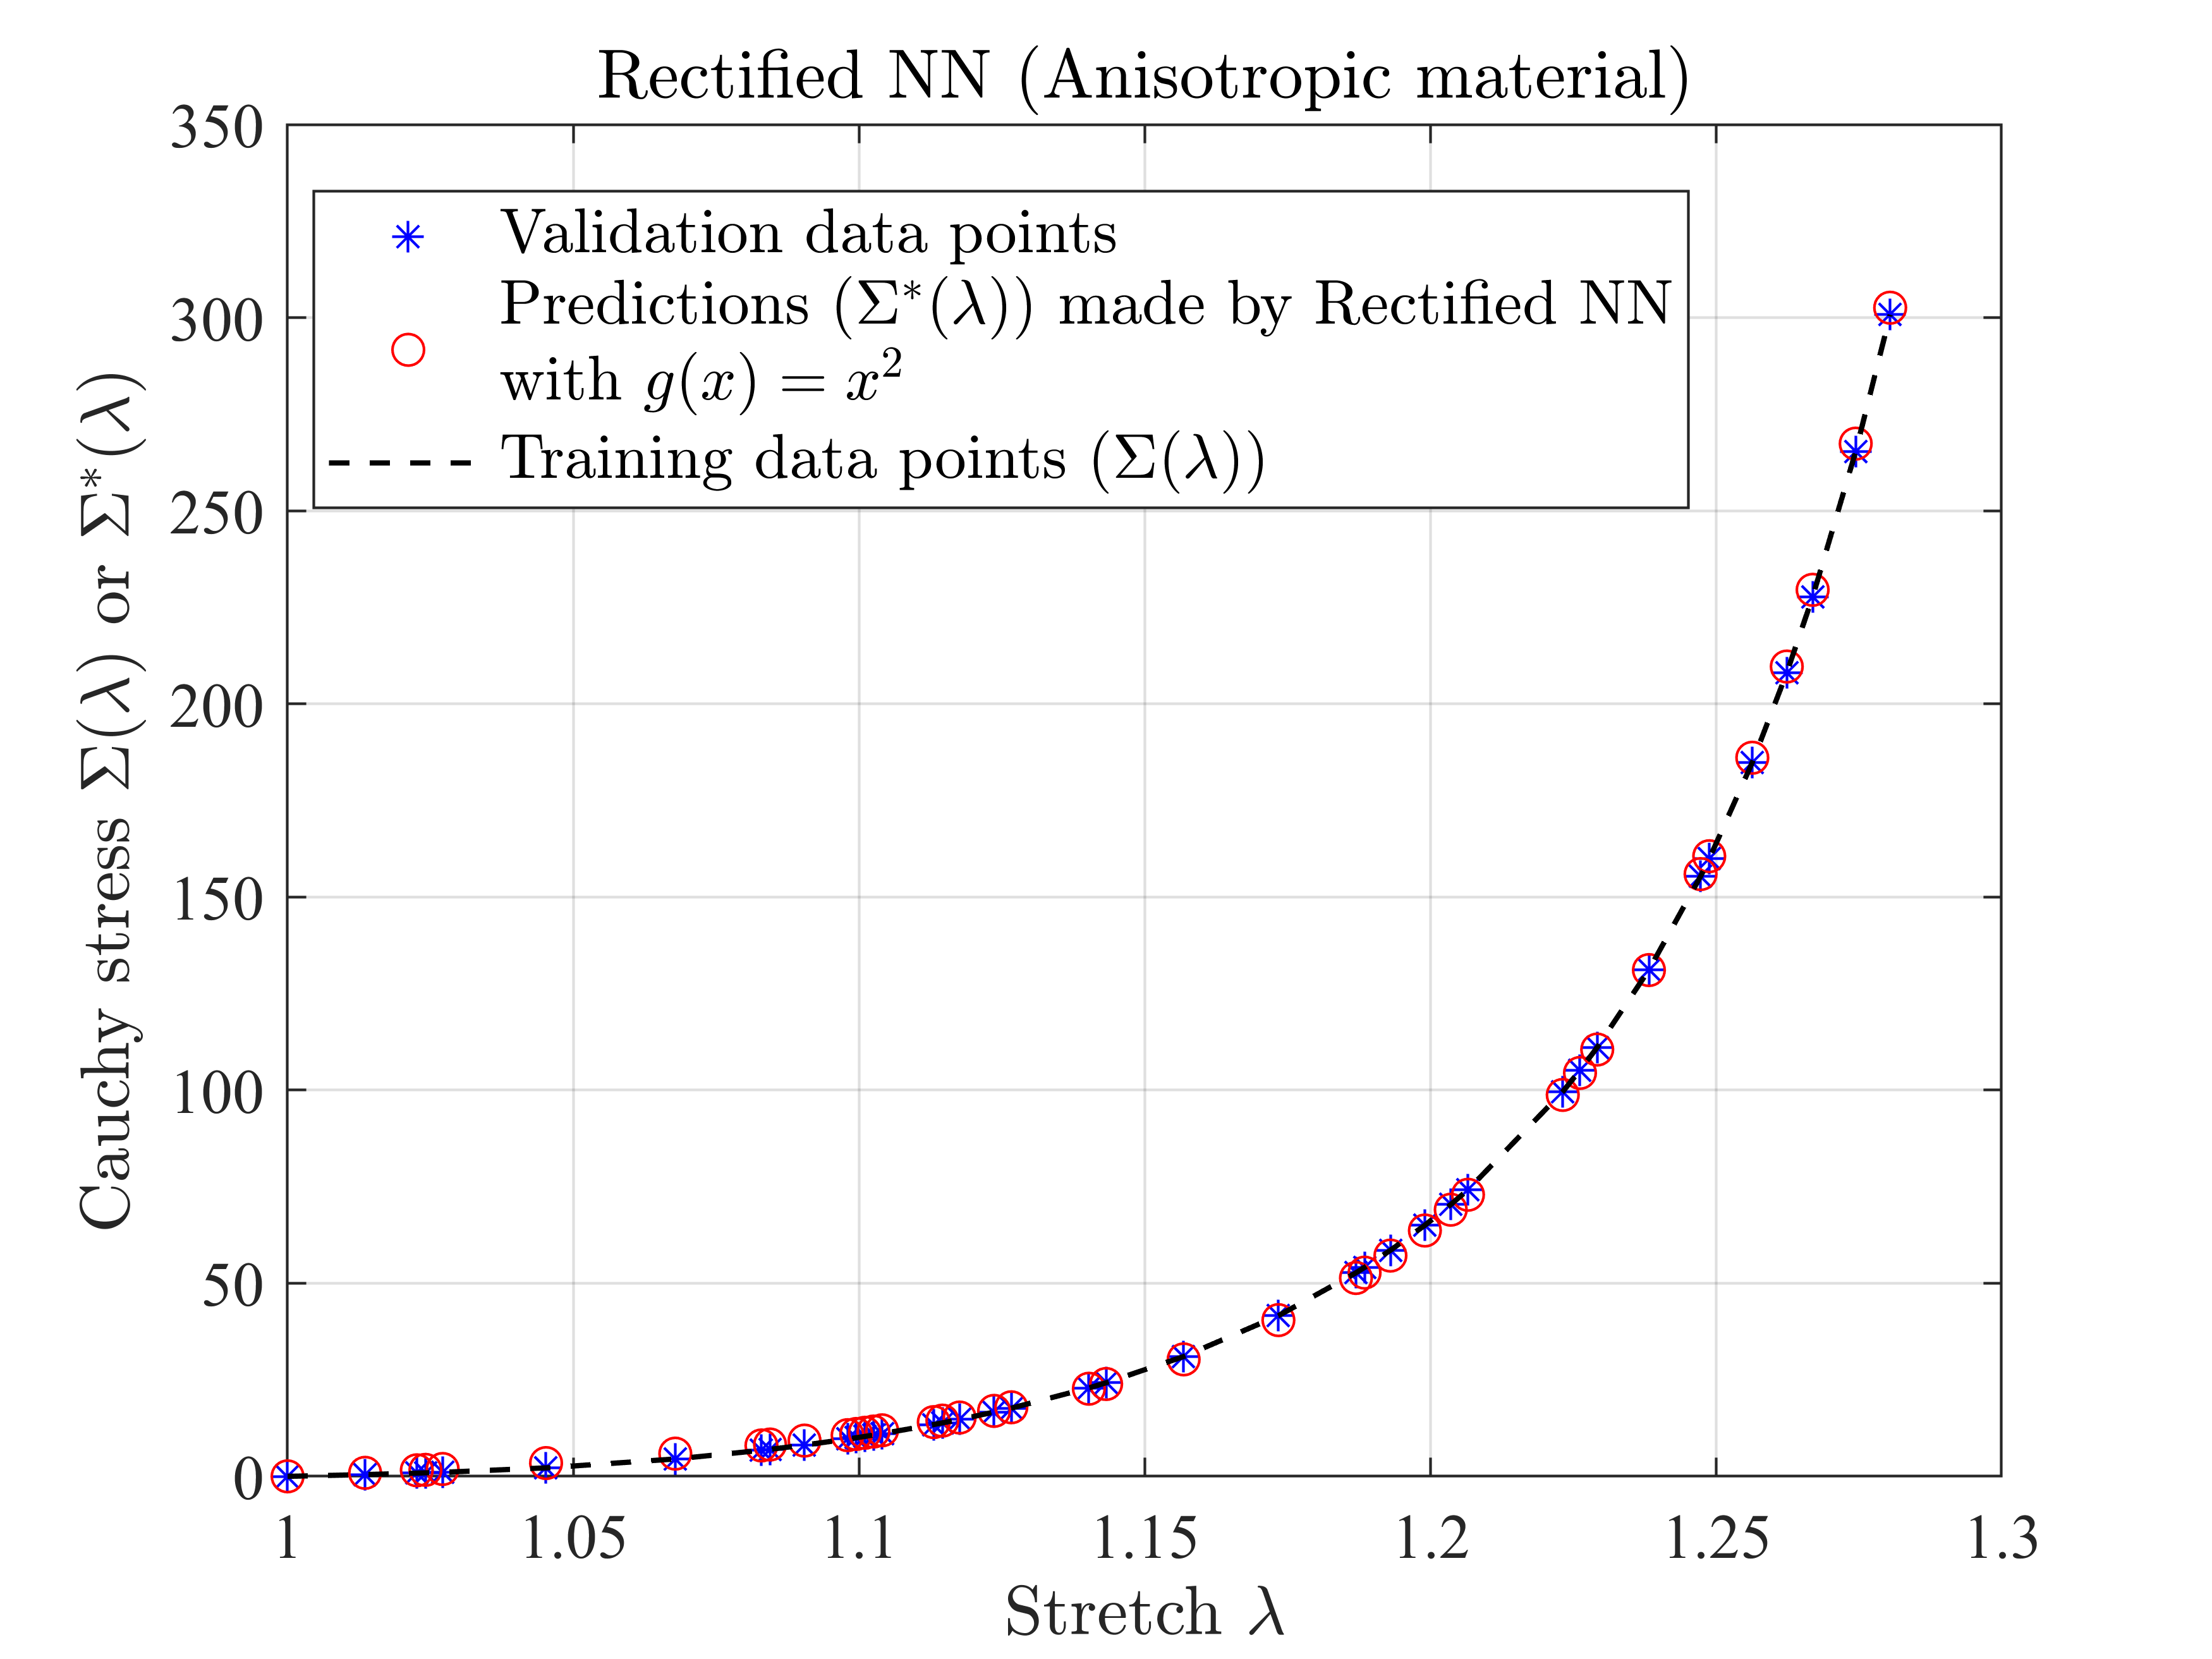
\includegraphics[width=0.5\textwidth]{Pictures/sigma_ANI.png}
    \end{center}
    \caption[Reference stress response and values, rectified NN predictions.]{Reference stress response $\lambda \mapsto \Sigma(\lambda)$ (black dashed line), reference values (blue star), and rectified neural network predictions (red circle) for the validation dataset (random selection). Here, the NN involves 4 hidden layers and 40 neurons per layer.}
    \label{fig:ANI best result 1}
\end{figure}
The validation metric in this example is $3.46 \times 10^{-6}$.

\subsection{Anisotropic Model for Experimental Dataset}\label{subsec:exp-app}
We finally apply the proposed rectification method to the experimental dataset presented in \cite{holzapfel2005determination}, corresponding to uniaxial extension tests on human illiac arterial walls. In those experiments, two different strips were harvested along the circumferential and longitudinal directions on each specimen to capture anisotropic effects. For the sake of illustration, two samples are randomly selected as target data for each layer defining the artery (adventitia, media, intima), and 10\% of the data is used as the validation dataset. The rectified neural network is similar to the one used in Section \ref{subsec:anisotropic-app} (see Eq.~\eqref{eq:rec-model-anisotropic-case}). 

Both axial and circumferential tension data are used for training. The Cauchy stress for the rectified model defined by Eq.~\eqref{eq:rec-model-anisotropic-case} in the circumferential direction reads as in Eq.~\eqref{eq:ANI_Cauchy}, in which
\begin{align}
    &\Sigma_1^*(\lambda) = 2 \frac{\partial w_1^*}{\partial I_1} \left(\lambda^2 - \frac{1}{\lambda}\right)\,, \\
    &\Sigma_2^*(\lambda) = 2 \frac{\partial w_2^*}{\partial I_2} \left(\lambda - \frac{1}{\lambda^2}\right)\,, \\
    &\Sigma_3^*(\lambda) = 2 \lambda^2 \frac{\partial w_3^*(J_4^{(1)})}{\partial J_4^{(1)}} \cos^2(\alpha)\,,
    \\
    &\Sigma_4^*(\lambda) = 2 \lambda^2 \frac{\partial w_4^*(J_4^{(2)})}{\partial J_4^{(2)}} \cos^2(\alpha)\,.
\end{align}
for uniaxial elongation.

The Cauchy stress for the tissue contribution in the longitudinal direction involves the terms
\begin{equation}
    \Sigma_3^*(\lambda) = 2 \lambda^2 \frac{\partial w_3^*(J_4^{(1)})}{\partial J_4^{(1)}} \sin^2(\alpha)
\end{equation}
and
\begin{equation}
    \Sigma_4^*(\lambda) = 2 \lambda^2 \frac{\partial w_4^*(J_4^{(2)})}{\partial J_4^{(2)}} \sin^2(\alpha)\,.
\end{equation}
The loss function in terms of datapoints is then defined as
\begin{align}
    \mathcal{L}_d = & \frac{\sum_{i=1}^{n_p^c} \left( \Sigma^{\text{exp}}(\lambda_{1}^c) - \Sigma^{*}(\lambda_{1}^c; \bfp) \right)^2}{\sum_{i=1}^{n_p^c} \Sigma^{\text{exp}}(\lambda_{1}^c)^2}  \nonumber \\ 
    & + \frac{\sum_{i=1}^{n_p^a} \left( \Sigma^{\text{exp}}(\lambda_{1}^a) - \Sigma^{*}(\lambda_{1}^a; \bfp) \right)^2}{\sum_{i=1}^{n_p^a} \Sigma^{\text{exp}}(\lambda_{1}^a)^2}\,,
\end{align}
where the superscripts ``c'' and ``a'' refer to data obtained by stretching along the circumferential and axial directions, respectively, $n_p^c$ and $n_p^a$ are the associated numbers of datapoints. As in Section \ref{subsec:anisotropic-app}, the stress free constraint is enforced in a strong sense by shifting the Cauchy stress.

Predictions obtained with the rectified neural network can be qualitatively compared with reference values in Fig.~\ref{fig:exp_circ} and Fig.~\ref{fig:exp_axial}, while validation errors can be found in Tab.~\ref{tab:val-err}. In this application, we used 2 hidden layers per neural network and 100 neurons per hidden layer. The rectified NN is trained for 2,000 epochs with a learning rate set to 0.01, then for 2,000 epochs with a learning rate taken as 0.001, and finally for 2,000 epochs at a learning rate set to 0.0001. 
\begin{figure}[ht!]
    \begin{center}
        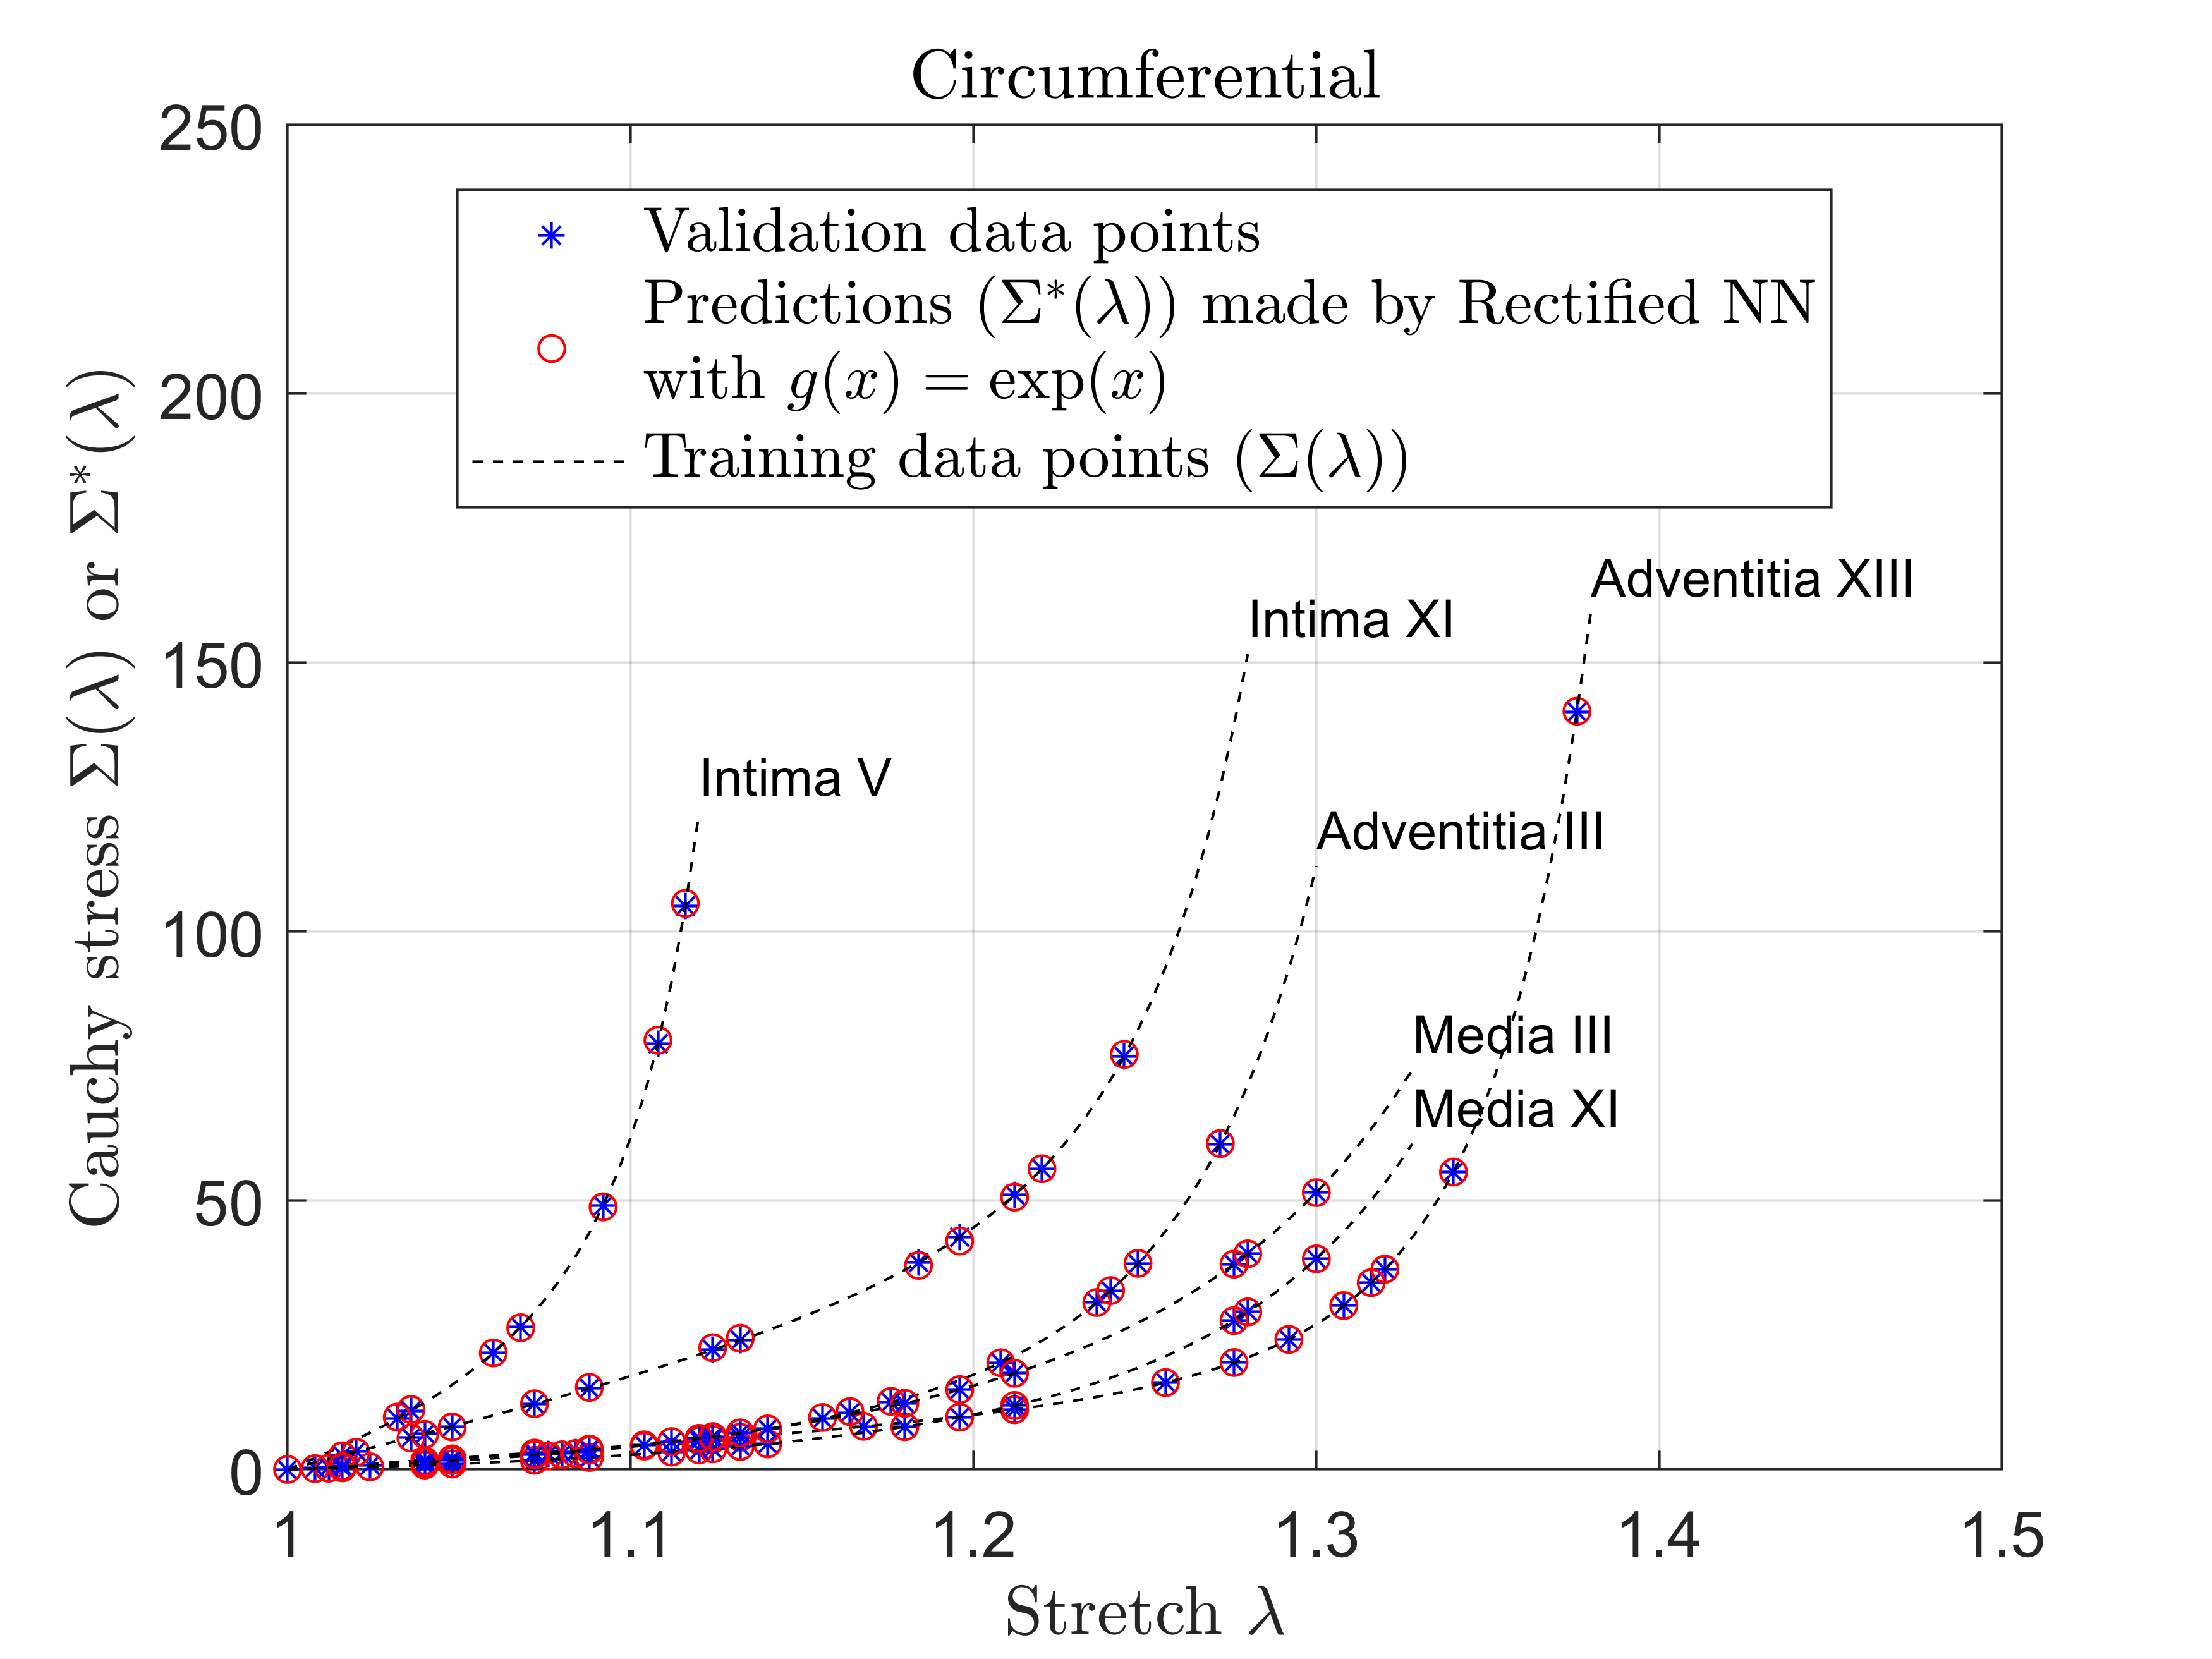
\includegraphics[width=0.5\textwidth]{Pictures/circ.png}
    \end{center}
    \caption[Reference stress response and values, RNN predictions (circumferential).]{Reference stress response $\lambda \mapsto \Sigma(\lambda)$ (black dashed line), reference values (blue star), and rectified neural network predictions (red circle) for the validation dataset in the circumferential direction (six experimental responses are considered for illustration purposes).}
    \label{fig:exp_circ}
\end{figure}
\begin{figure}[ht!]
    \begin{center}
        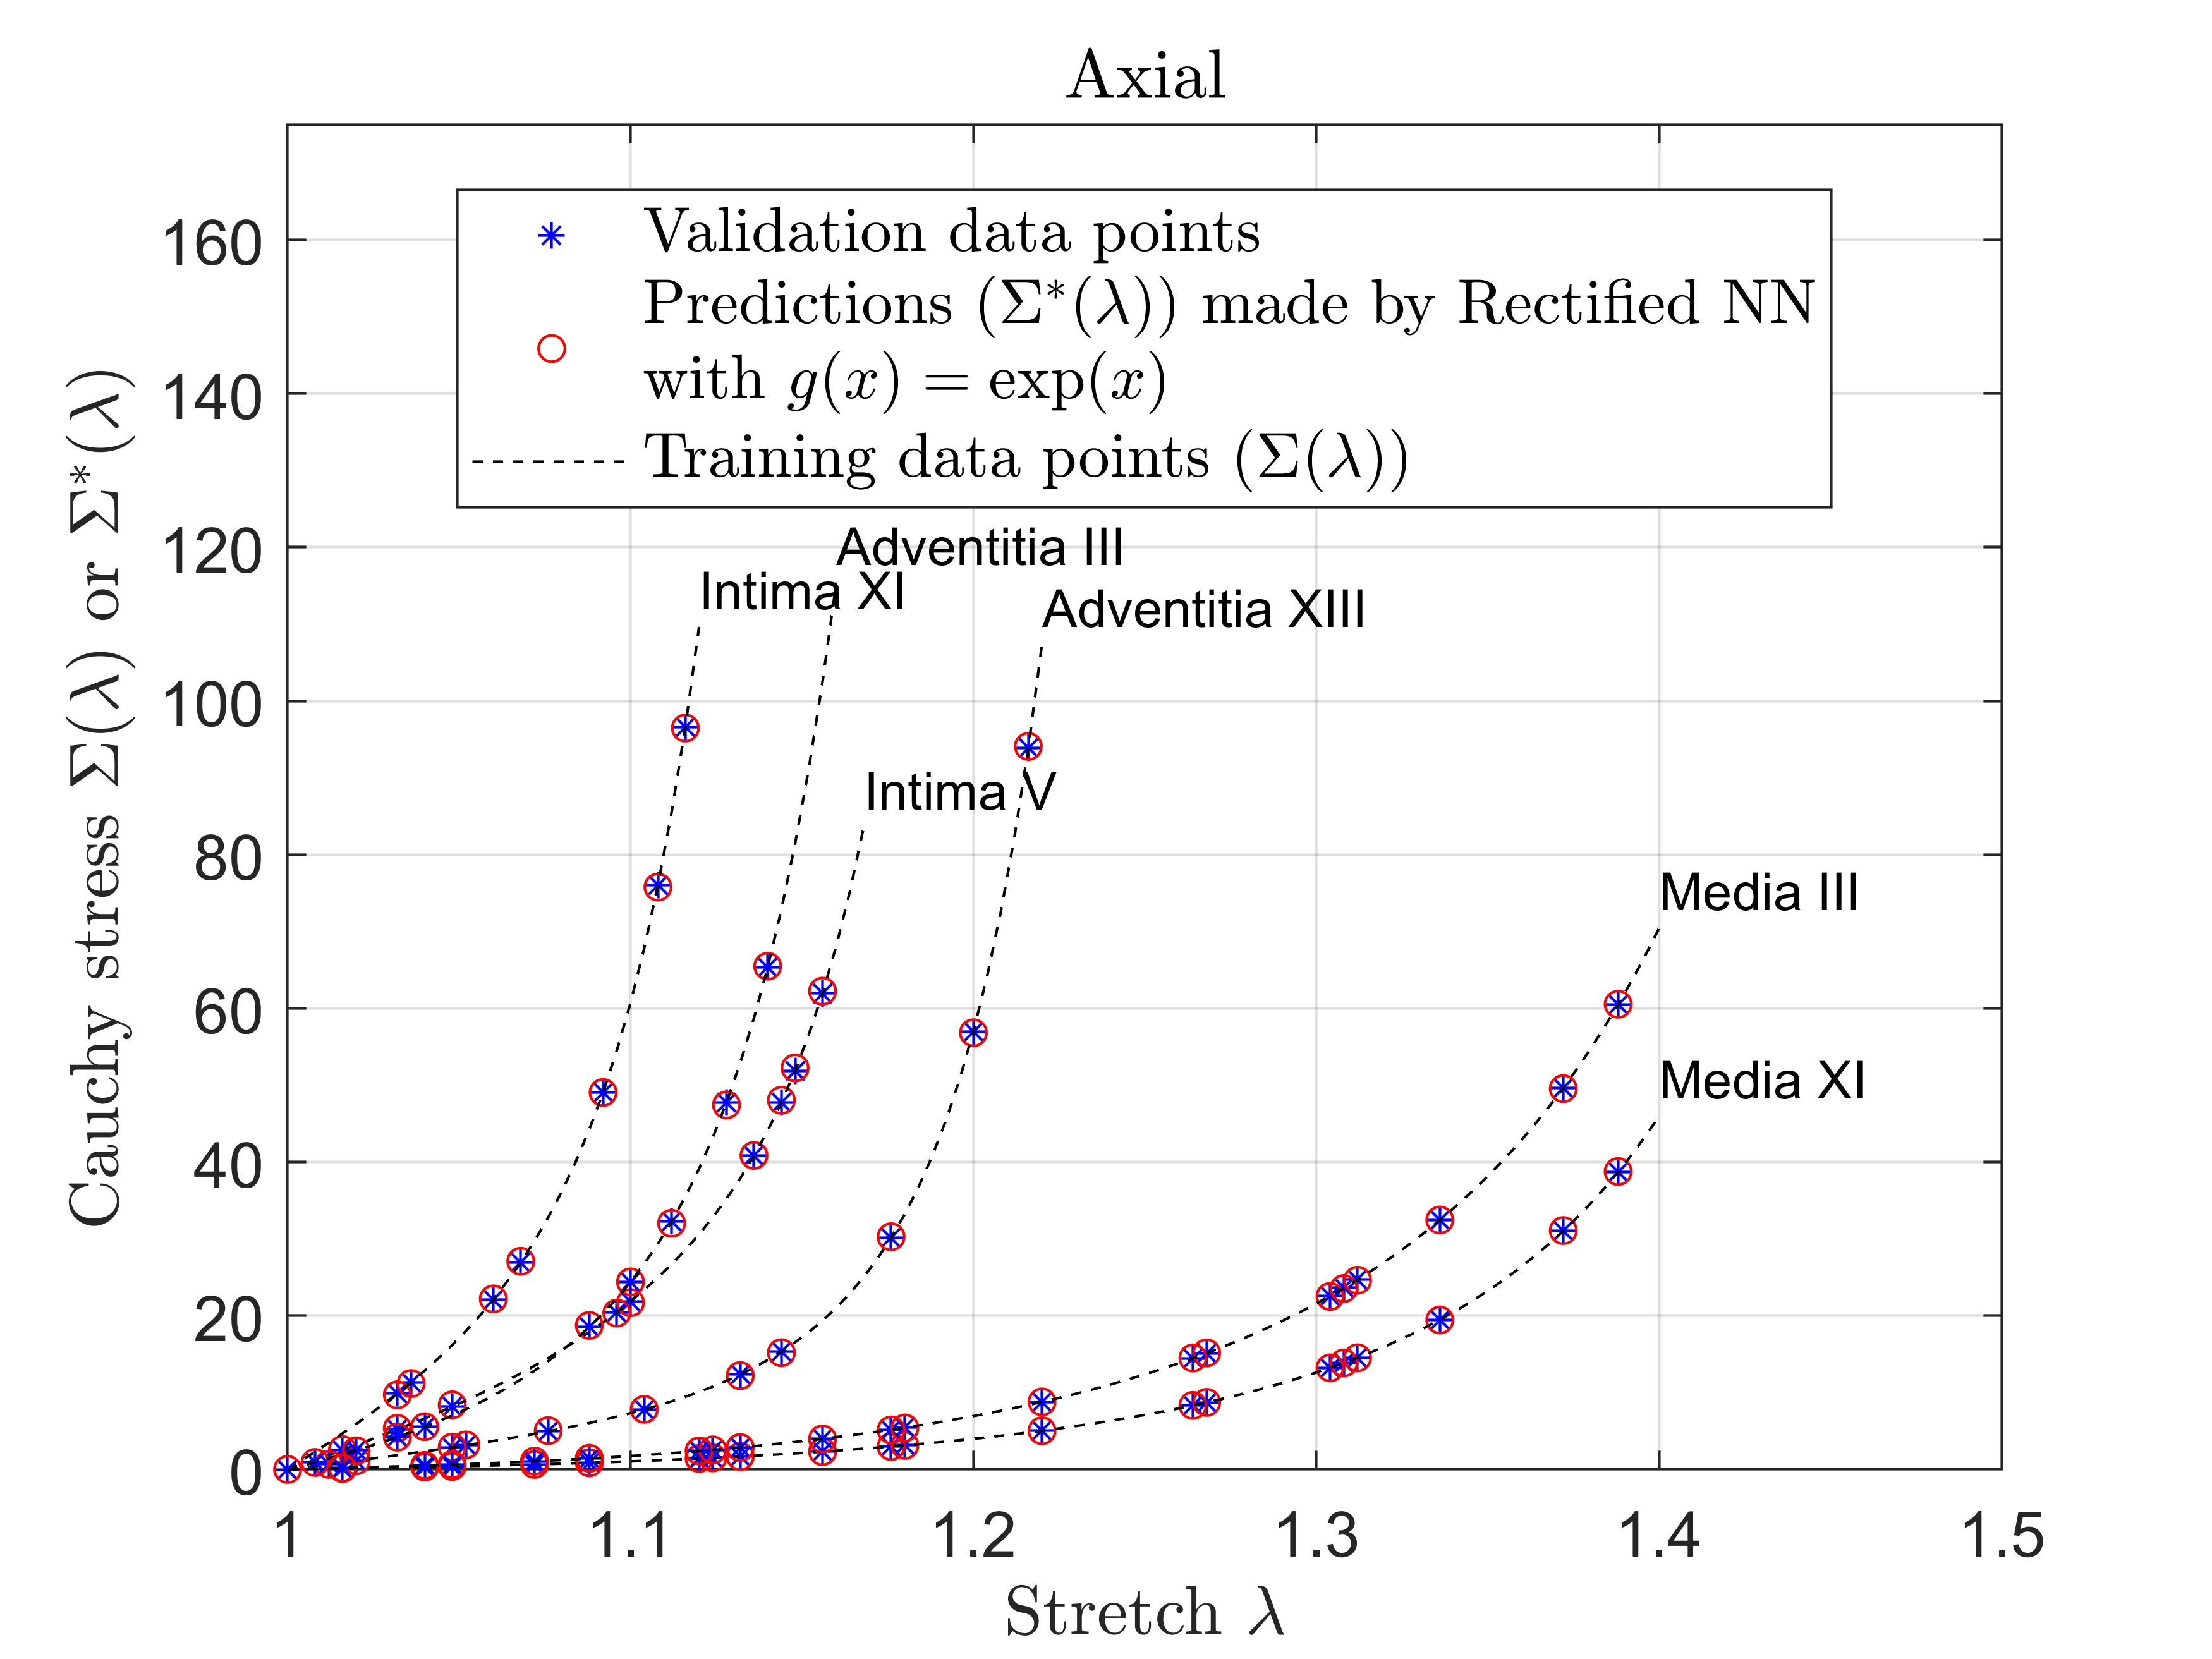
\includegraphics[width=0.5\textwidth]{Pictures/axial.png}
    \end{center}
    \caption[Reference stress response and reference values, RNN predictions (axial).]{Reference stress response $\lambda \mapsto \Sigma(\lambda)$ (black dashed line), reference values (blue star), and rectified neural network predictions (red circle) for the validation dataset in the axial direction (six experimental responses are considered for illustration purposes).}
    \label{fig:exp_axial}
\end{figure}
With a maximal validation error equal to $1.0096\times10^{-4}$ (obtained for sample \#XI, intima layer), it is seen that the rectified neural network can reproduce the experimental data very well, for all different layers in the two directions.

\begin{table}[ht!]
\caption[Validation errors for each sample.]{Validation errors for each sample. Specimen numbers are those reported in \cite{holzapfel2005determination}.}
\label{tab:val-err}
\begin{center}
    \begin{tabular}{|c|c|} 
 \hline
 Layer/Specimen number & Error $\mathcal{L}_d$ $\times 10^{-4}$ \\
 \hline
 Adventitia/\#III & 0.9972 \\
 Adventitia/\#XIII & 0.1331 \\
 Intima/\#V & 0.7994 \\
 Intima/\#XI & 1.0096 \\
 Media/\#III & 0.0252 \\
 Media/\#XI & 0.0355 \\
 \hline
\end{tabular}
\end{center}

\end{table}

\chapter{Nonsense text for layout proofing}
\label{hello}

Enjoy some Lorem Ipsum text!
This should create about two full pages of text so you can verify the
margins are correct (especially if you're doing two-sided).

\section{Lorem Ipsum}
Lorem ipsum dolor sit amet, consectetuer adipiscing elit. Sed vitae leo.
Pellentesque quis nisi id orci consectetuer posuere. Quisque malesuada
rhoncus dui. Vivamus mi. Mauris commodo. Phasellus lacus magna, feugiat ac,
blandit ut, rutrum id, massa. In consectetuer magna vel justo. Cras eu
diam. Nullam tortor turpis, bibendum non, consequat ac, tincidunt non,
nisi. 

Curabitur sagittis dignissim arcu. Pellentesque habitant morbi
tristique senectus et netus et malesuada fames ac turpis egestas.
Vestibulum ullamcorper. Curabitur faucibus euismod nulla. Vivamus sagittis.
Sed fermentum neque a risus vestibulum convallis. Morbi id massa ut arcu
mollis commodo. Aliquam erat volutpat.  Pellentesque fringilla pellentesque
nisi. Morbi tristique ornare libero. Vestibulum turpis sapien, iaculis ut,
cursus non, condimentum in, tortor. Aenean vehicula. Integer egestas
tincidunt erat. Aenean euismod ante vel lectus. Duis ac sapien vel erat
euismod aliquet. Vivamus tempor placerat nibh. Curabitur pharetra, orci
consequat pulvinar ultricies, orci enim tempor augue, non lacinia orci nisl
et nibh. Nunc gravida dictum turpis.  Duis sollicitudin commodo massa. Nam
ac nunc. Fusce sodales posuere velit. Nunc ullamcorper sodales urna. Donec
consectetuer accumsan ante. Morbi feugiat rutrum mauris. Praesent malesuada
auctor est. Pellentesque quis odio non nulla ornare imperdiet. Aliquam
dapibus. Suspendisse posuere, magna in molestie varius, ipsum velit rhoncus
nisi, nec bibendum pede mauris in urna. Morbi purus lectus, molestie quis,
laoreet id, tincidunt at, ligula. 

Praesent sit amet libero id arcu
adipiscing tristique. Quisque libero erat, bibendum nec, malesuada in,
gravida et, urna. Phasellus molestie vulputate nisi. Nullam massa magna,
dignissim ac, accumsan a, scelerisque eu, erat. Nam tellus augue, tempus
nec, molestie sit amet, rhoncus vel, libero. Vestibulum at neque. Aliquam
laoreet tincidunt mi. Ut laoreet ligula ac urna. Nullam nisl pede, posuere
id, dictum a, fermentum vitae, turpis.  Nulla ante mauris, euismod et,
mollis eu, tempor in, quam. 

In pede augue, elementum varius, tincidunt in,
condimentum ut, erat. Etiam vulputate faucibus velit. Aliquam porttitor.
Nam fringilla adipiscing nisi. Sed in magna. Aenean non ante. Aenean
facilisis, nunc sed aliquam porta, magna est aliquam nisi, vitae semper
turpis orci ac dolor. Praesent nec tellus. Cras vulputate rhoncus sem.
Curabitur eu mi. Mauris euismod lacinia nibh. Suspendisse eget sapien et
nunc accumsan elementum.  Nulla dapibus. Donec interdum elit mattis velit
imperdiet aliquet. Mauris feugiat, ante vel faucibus rutrum, eros mauris
sollicitudin neque, ut varius diam ipsum et massa. Nullam non nisi sit amet
tortor rhoncus molestie. Cras consectetuer condimentum ante. Phasellus
fermentum risus fermentum turpis. Mauris dignissim iaculis sem. Fusce nisi
lorem, viverra id, auctor et, scelerisque ut, massa. In hac habitasse
platea dictumst. Vestibulum ante ipsum primis in faucibus orci luctus et
ultrices posuere cubilia Curae; Aliquam pulvinar neque ac dolor.

\section{More nonsense}
Lorem ipsum dolor sit amet, consectetuer adipiscing elit. Sed vitae leo.
Pellentesque quis nisi id orci consectetuer posuere. Quisque malesuada
rhoncus dui. Vivamus mi. Mauris commodo. Phasellus lacus magna, feugiat ac,
blandit ut, rutrum id, massa. In consectetuer magna vel justo. Cras eu
diam. Nullam tortor turpis, bibendum non, consequat ac, tincidunt non,
nisi. 
Curabitur sagittis dignissim arcu. Pellentesque habitant morbi
tristique senectus et netus et malesuada fames ac turpis egestas.

Vestibulum ullamcorper. Curabitur faucibus euismod nulla. Vivamus sagittis.
Sed fermentum neque a risus vestibulum convallis. Morbi id massa ut arcu
mollis commodo. Aliquam erat volutpat.  Pellentesque fringilla pellentesque
nisi. Morbi tristique ornare libero. Vestibulum turpis sapien, iaculis ut,
cursus non, condimentum in, tortor. Aenean vehicula. 

Integer egestas
tincidunt erat. Aenean euismod ante vel lectus. Duis ac sapien vel erat
euismod aliquet. Vivamus tempor placerat nibh. Curabitur pharetra, orci
consequat pulvinar ultricies, orci enim tempor augue, non lacinia orci nisl
et nibh. Nunc gravida dictum turpis.  Duis sollicitudin commodo massa. Nam
ac nunc. Fusce sodales posuere velit. Nunc ullamcorper sodales urna. Donec
consectetuer accumsan ante. Morbi feugiat rutrum mauris. Praesent malesuada
auctor est. 

Pellentesque quis odio non nulla ornare imperdiet. Aliquam
dapibus. Suspendisse posuere, magna in molestie varius, ipsum velit rhoncus
nisi, nec bibendum pede mauris in urna. Morbi purus lectus, molestie quis,
laoreet id, tincidunt at, ligula. 
Praesent sit amet libero id arcu
adipiscing tristique. Quisque libero erat, bibendum nec, malesuada in,
gravida et, urna. Phasellus molestie vulputate nisi. Nullam massa magna,
dignissim ac, accumsan a, scelerisque eu, erat. Nam tellus augue, tempus
nec, molestie sit amet, rhoncus vel, libero. Vestibulum at neque. Aliquam
laoreet tincidunt mi. Ut laoreet ligula ac urna. Nullam nisl pede, posuere
id, dictum a, fermentum vitae, turpis.  Nulla ante mauris, euismod et,
mollis eu, tempor in, quam. 
In pede augue, elementum varius, tincidunt in,
condimentum ut, erat. Etiam vulputate faucibus velit. Aliquam porttitor.

Nam fringilla adipiscing nisi. Sed in magna. Aenean non ante. Aenean
facilisis, nunc sed aliquam porta, magna est aliquam nisi, vitae semper
turpis orci ac dolor. Praesent nec tellus. Cras vulputate rhoncus sem.
Curabitur eu mi. Mauris euismod lacinia nibh. Suspendisse eget sapien et
nunc accumsan elementum.  Nulla dapibus. Donec interdum elit mattis velit
imperdiet aliquet. Mauris feugiat, ante vel faucibus rutrum, eros mauris
sollicitudin neque, ut varius diam ipsum et massa. Nullam non nisi sit amet
tortor rhoncus molestie. Cras consectetuer condimentum ante. Phasellus
fermentum risus fermentum turpis. Mauris dignissim iaculis sem. Fusce nisi
lorem, viverra id, auctor et, scelerisque ut, massa. In hac habitasse
platea dictumst. Vestibulum ante ipsum primis in faucibus orci luctus et
ultrices posuere cubilia Curae; Aliquam pulvinar neque ac dolor.

\chapter{Conclusions}

In Chapter~\ref{chap:artery}, we developed a stochastic model for spatially-dependent anisotropic strain energy density functions. A least-informative model was obtained by applying the maximum entropy principle under constraints related to existence theorems in finite elasticity. This approach therefore ensures that the associated nonlinear boundary value problem is well posed almost surely. Information related to model linearization was also integrated and generate statistical dependencies in the variables parameterizing the stochastic strain energy density function. The identification of the model was performed using a database on human arteries, available in the literature. Here, maximum likelihood estimators were obtained and are provided for the three layers constituting the arterial wall. Finally, uncertainty propagation on a realistic, patient-specific geometry was conducted to demonstrate some capabilities of the stochastic modeling framework.

Avenues for future work include the use of the proposed framework to derive generative models for data-driven methodologies, the integration of the active response exhibited by arteries in in-vivo conditions, as well as refined identification using nondestructive techniques resolving spatial scales.

In Chapter~\ref{chap:polyconvex}, a method to correct unconstrained neural networks for hyperelastic models was proposed. The approach relies on a composite mapping that transforms any function into a convex function, hence ensuring the polyconvexity of the neural network---without constraints on the weights and  activation functions. 

The strategy was first illustrated on a toy problem to characterize the impact of the positive function used to enforce monotonicity (in terms of accuracy and training effort). The rectified NN models were then deployed on digitally synthesized and experimental datasets, relevant to both isotropic and anisotropic materials. Good fitting capabilities were observed in all applications. It was shown that the proposed rectified models typically convergence faster than \textit{a priori} constrained models, at the expense of a greater computational cost per iteration. 

Avenues for future research include the generalization to other types of strain energy density functions, as well as more extensive comparisons with \textit{a priori} constrained representations. 

%==============================================================================

%-----------------------------------------------------------------------------%
% APPENDICES -- OPTIONAL. These are just chapters enumerated by Appendix A,
%                Appendix B, Appendix C...
%-----------------------------------------------------------------------------%
\begin{appendices}
	\titleformat{\chapter}[block]
	{
		\usefont{T1}{phv}{b}{n}\fontsize{16pt}{\normalbaselines}
		\normalbaselines
		\usefont{T1}{phv}{b}{n}\fontsize{16pt}{\normalbaselineskip}}
	{Appendix \thechapter.}{.2em}{\normalbaselines}
	\titlespacing\chapter{0pt}{-10pt plus 4pt minus 0pt}{6pt plus 2pt minus 0pt}
	
	\appendixtitleon

\chapter{Artery}

\section{code verification}
\label{app:VV-artery}


In this work, code verification is performed by considering a cube $B = [0,1]^3$ and a manufactured displacement field taken as 
\begin{equation}
    \bfu^{\textnormal{MMS}}(\bfx) = (-0.01\exp(x_3), 0, 0)^T\,.
\end{equation}
Dirichlet boundary conditions in accordance with the above solution are prescribed on all boundaries. A body force is defined such that the manufactured solution corresponds to the nonlinear boundary value problem defined in Section \ref{subsec:def-NBVP}. The convergence order is measured by the $L^2$-norm of the difference between the approximation and the manufactured solution. The $h$-convergence of the norm is shown in Fig.~\ref{fig:mms}, and a third-order convergence rate is observed as expected.
\begin{figure}[ht!]
    \begin{center}
        \includegraphics[trim = {2cm 9cm 2cm 9cm}, clip, width = 0.6\textwidth]{MMS-Convergence.pdf}
    \end{center}
    \caption[Convergence of the $L^2$ error for the manufactured solution.]{Convergence of the $L^2$ error ($h$-refinement) for the manufactured solution.}
    \label{fig:mms}
\end{figure}

\section{Strategy for Solving the Fractional Stochastic Partial Differential Equation}\label{sec:solver-SPDE}
For the sake of self-consistency, the numerical strategy to solve the anisotropic fractional stochastic partial differential equation
\begin{equation}
    (\gamma^2 \mathcal{I} -\langle \nabla, \bs{D}\nabla\rangle)^{\alpha/2} U = \dot{W}\,,
    \label{eq:spdeH-app}
\end{equation}
is recalled in this appendix. Following \cite{Lindgren2011}, a finite-dimensional representation associated with a set $\{\psi_i\}_{i=1}^{N}$ of piecewise linear basis functions (with a mesh comprising $N$ nodes) is introduced as follows:
\begin{equation}
U(\bs{x}) = \sum_{i=1}^{N} U_i \psi_i(\bs{x})\,.
\end{equation}
Let $\bs{U} = (U_1, \ldots, U_N)^T$ be the Gaussian random vector of nodal values. For $\alpha = 2$, it was shown in the above reference that the weak Galerkin stochastic solution satisfies
\begin{equation}
    \bs{U} \sim \mathcal{N}(\bs{0}_N, \bs{\Sigma})\,,
\end{equation}
where the covariance matrix $\bs{\Sigma}$ is given by 
\begin{equation}
    \bs{\Sigma} = \left(\kappa^2 \bs{M} + \bs{G}\right)^{-1} \bs{M} \left(\kappa^2 \bs{M} + \bs{G}\right)^{-1}]\,,
\end{equation} 
with
\begin{equation}
M_{ij} = \int_{\Omega} \psi_i(\bs{x})\psi_j(\bs{x})\,d\bs{x}
\label{eq:M}
\end{equation}
and
\begin{equation}
G_{ij} = \int_{\Omega} \langle \bs{\nabla}\psi_i(\bs{x}), \bs{D}(\bs{x})\bs{\nabla}\psi_j(\bs{x})\rangle \, d\bs{x}
\end{equation}
for $1 \leqslant i,j \leqslant N$, respectively. For computational efficiency, the sampling task is then usually recast using the precision matrix 
\begin{equation}
    \bs{\Sigma}^{-1} = \left(\kappa^2 \bs{M} + \bs{G}\right) \bs{M}^{-1} \left(\kappa^2 \bs{M} + \bs{G}\right)\,,
\end{equation}
where $\bs{M}^{-1}$ can be evaluated by applying a lumping procedure. For $\alpha \neq 2$, recursive formula can be applied, see \cite{Lindgren2011}.


\section{Reduced-Order Model Solutions}
In this Appendix, additional solution snapshots are provided, together with absolute errors, to assess the accuracy of the presented frameworks.
\begin{figure}[!htb]
     \begin{center}
        \begin{subfigure}[b]{0.23\textwidth}
            \begin{center}
                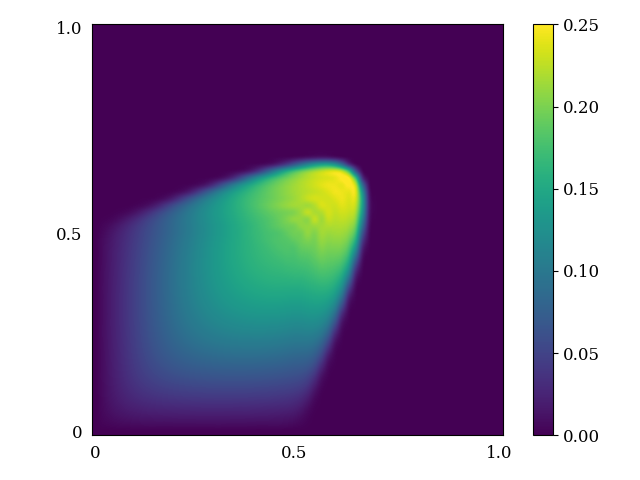
\includegraphics[trim = {0, 0, 3cm, 0}, clip, width=\textwidth]{X-rom-LE-DAE-5.png}
            \end{center}
            \caption{Solution $r = 5$}
        \end{subfigure}
   \begin{subfigure}[b]{0.23\textwidth}
            \begin{center}
                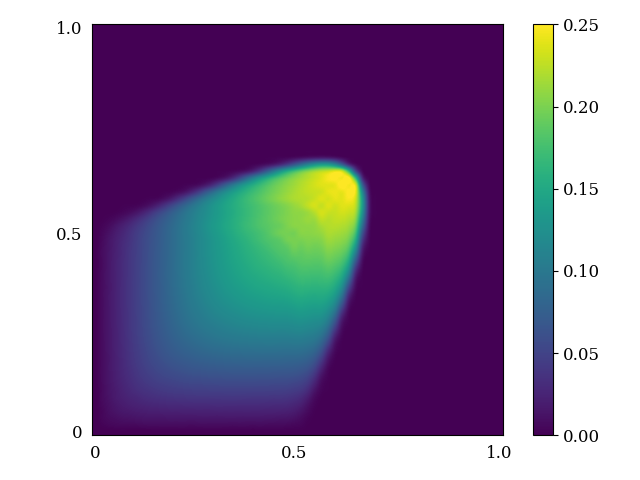
\includegraphics[trim = {0, 0, 3cm, 0}, clip, width=\textwidth]{X-rom-LE-DAE-10.png}
            \end{center}
            \caption{Solution $r = 10$}
        \end{subfigure}
   \begin{subfigure}[b]{0.23\textwidth}
            \begin{center}
                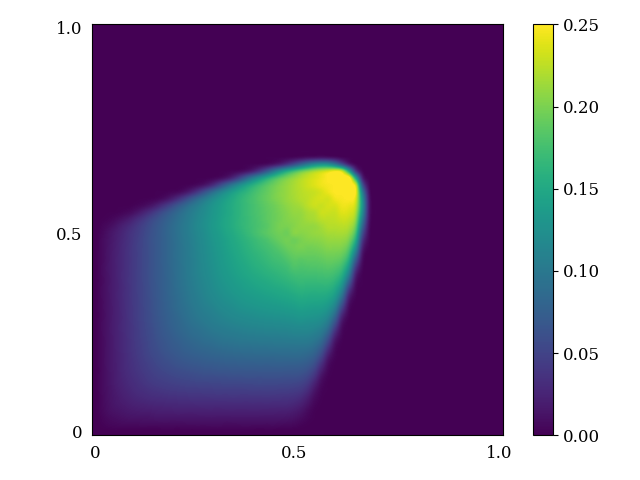
\includegraphics[trim = {0, 0, 3cm, 0}, clip, width=\textwidth]{X-rom-LE-DAE-15.png}
            \end{center}
            \caption{Solution $r = 15$}
        \end{subfigure}
   \begin{subfigure}[b]{0.23\textwidth}
            \begin{center}
                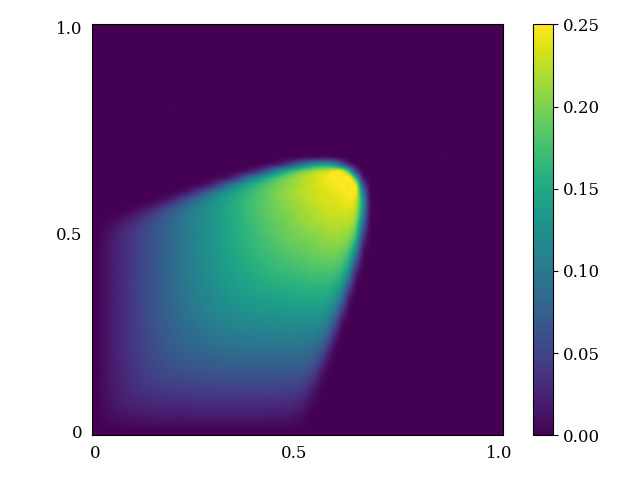
\includegraphics[trim = {0, 0, 3cm, 0}, clip, width=\textwidth]{X-rom-LE-DAE-20.png}
            \end{center}
            \caption{Solution $r = 20$}
        \end{subfigure}\\  
        \begin{subfigure}[b]{0.23\textwidth}
            \begin{center}
                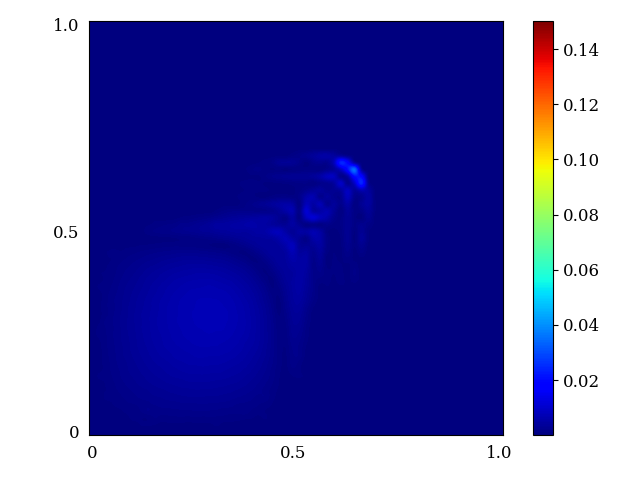
\includegraphics[trim = {0, 0, 3cm, 0}, clip, width=\textwidth]{X-rom-LE-DAE-5-abs-err.png}
            \end{center}
            \caption{Absolute error $r = 5$}
        \end{subfigure}  
        \begin{subfigure}[b]{0.23\textwidth}
            \begin{center}
                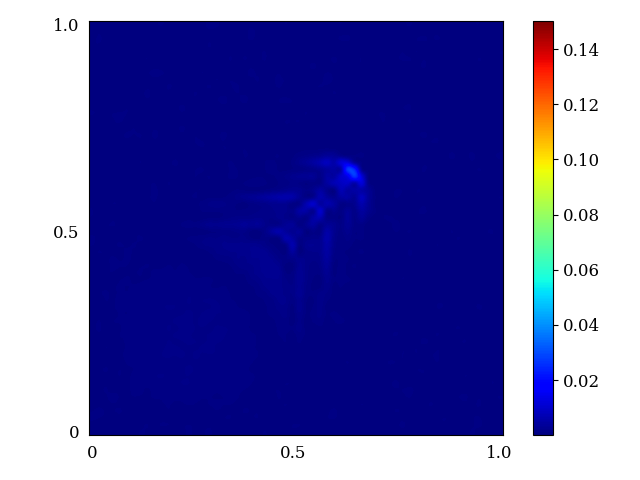
\includegraphics[trim = {0, 0, 3cm, 0}, clip, width=\textwidth]{X-rom-LE-DAE-10-abs-err.png}
            \end{center}
            \caption{Absolute error $r = 10$}
        \end{subfigure}   
        \begin{subfigure}[b]{0.23\textwidth}
            \begin{center}
                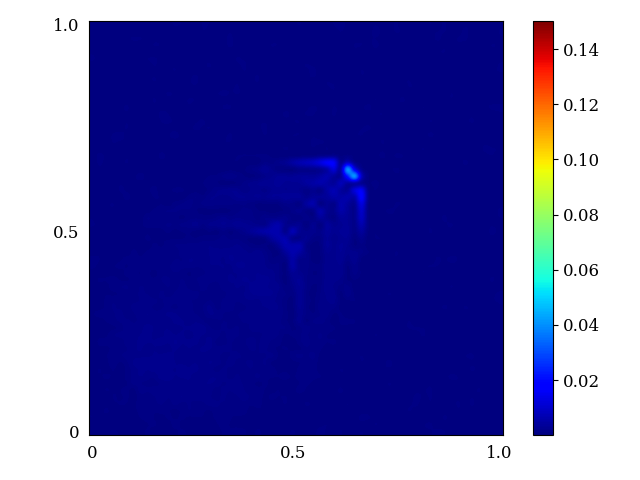
\includegraphics[trim = {0, 0, 3cm, 0}, clip, width=\textwidth]{X-rom-LE-DAE-15-abs-err.png}
            \end{center}
            \caption{Absolute error $r = 15$}
        \end{subfigure}    
        \begin{subfigure}[b]{0.23\textwidth}
            \begin{center}
                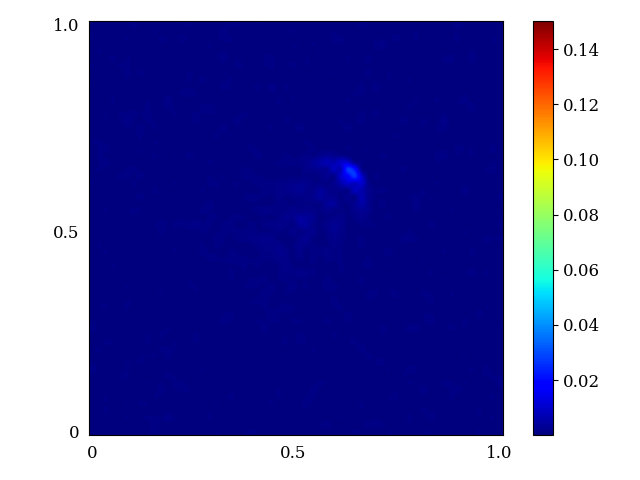
\includegraphics[trim = {0, 0, 3cm, 0}, clip, width=\textwidth]{X-rom-LE-DAE-20-abs-err.png}
            \end{center}
            \caption{Absolute error $r = 20$}
        \end{subfigure}
     \end{center}
     \caption[Solutions and pointwise errors for LE-DAE-DNNOp.]{Solutions (a, b, c, d) and pointwise errors (e, f, g, h) for LE-DAE-DNNOp with different latent space dimensions.}
        \label{fig: ledae-burger}
\end{figure}

\begin{figure}[!htb]
     \begin{center}
        \begin{subfigure}[b]{0.23\textwidth}
            \begin{center}
                \includegraphics[trim = {0, 0, 3cm, 0}, clip, width=\textwidth]{X-rom-LE-SAE-5.png}
            \end{center}
            \caption{Solution $r = 5$}
        \end{subfigure}
   \begin{subfigure}[b]{0.23\textwidth}
        \begin{center}
            \includegraphics[trim = {0, 0, 3cm, 0}, clip, width=\textwidth]{X-rom-LE-SAE-10.png}
        \end{center}
            \caption{Solution $r = 10$}
        \end{subfigure}
   \begin{subfigure}[b]{0.23\textwidth}
       \begin{center}
        \includegraphics[trim = {0, 0, 3cm, 0}, clip, width=\textwidth]{X-rom-LE-SAE-15.png}
       \end{center}
            \caption{Solution $r = 15$}
        \end{subfigure}
   \begin{subfigure}[b]{0.23\textwidth}
       \begin{center}
        \includegraphics[trim = {0, 0, 3cm, 0}, clip, width=\textwidth]{X-rom-LE-SAE-20.png}
       \end{center}
            \caption{Solution $r = 20$}
        \end{subfigure}\\  
        \begin{subfigure}[b]{0.23\textwidth}
            \begin{center}
                \includegraphics[trim = {0, 0, 3cm, 0}, clip, width=\textwidth]{X-rom-LE-SAE-5-abs-err.png}
            \end{center}
            \caption{Absolute error $r = 5$}
        \end{subfigure}  
        \begin{subfigure}[b]{0.23\textwidth}
            \begin{center}
                \includegraphics[trim = {0, 0, 3cm, 0}, clip, width=\textwidth]{X-rom-LE-SAE-10-abs-err.png}
            \end{center}
            \caption{Absolute error $r = 10$}
        \end{subfigure}   
        \begin{subfigure}[b]{0.23\textwidth}
            \begin{center}
                \includegraphics[trim = {0, 0, 3cm, 0}, clip, width=\textwidth]{X-rom-LE-SAE-15-abs-err.png}
            \end{center}
            \caption{Absolute error $r = 15$}
        \end{subfigure}    
        \begin{subfigure}[b]{0.23\textwidth}
            \begin{center}
                \includegraphics[trim = {0, 0, 3cm, 0}, clip, width=\textwidth]{X-rom-LE-SAE-20-abs-err.png}
            \end{center}
            \caption{Absolute error $r = 20$}
        \end{subfigure}
     \end{center}
     \caption[Solutions and pointwise errors for LE-SAE-DNNOp.]{Solutions (a, b, c, d) and pointwise errors (e, f, g, h) for LE-SAE-DNNOp with different latent space dimensions.}
        \label{fig: lesae-burger}
\end{figure}


\begin{figure}[!htb]
     \begin{center}
        \begin{subfigure}[b]{0.23\textwidth}
            \begin{center}
                \includegraphics[trim = {0, 0, 3cm, 0}, clip, width=\textwidth]{X-rom-LE-CNNAE-5.png}
            \end{center}
             \caption{Solution $r = 5$}
         \end{subfigure}
    \begin{subfigure}[b]{0.23\textwidth}
            \begin{center}
                \includegraphics[trim = {0, 0, 3cm, 0}, clip, width=\textwidth]{X-rom-LE-CNNAE-10.png}
            \end{center}
             \caption{Solution $r = 10$}
         \end{subfigure}
    \begin{subfigure}[b]{0.23\textwidth}
            \begin{center}
                \includegraphics[trim = {0, 0, 3cm, 0}, clip, width=\textwidth]{X-rom-LE-CNNAE-15.png}
            \end{center}
             \caption{Solution $r = 15$}
         \end{subfigure}
    \begin{subfigure}[b]{0.23\textwidth}
            \begin{center}
                \includegraphics[trim = {0, 0, 3cm, 0}, clip, width=\textwidth]{X-rom-LE-CNNAE-20.png}
            \end{center}
             \caption{Solution $r = 20$}
         \end{subfigure}\\  
         \begin{subfigure}[b]{0.23\textwidth}
             \begin{center}
                \includegraphics[trim = {0, 0, 3cm, 0}, clip, width=\textwidth]{X-rom-LE-CNNAE-5-abs-err.png}
             \end{center}
             \caption{Absolute error $r = 5$}
         \end{subfigure}  
         \begin{subfigure}[b]{0.23\textwidth}
             \begin{center}
                \includegraphics[trim = {0, 0, 3cm, 0}, clip, width=\textwidth]{X-rom-LE-CNNAE-10-abs-err.png}
             \end{center}
             \caption{Absolute error $r = 10$}
         \end{subfigure}   
         \begin{subfigure}[b]{0.23\textwidth}
             \begin{center}
                \includegraphics[trim = {0, 0, 3cm, 0}, clip, width=\textwidth]{X-rom-LE-CNNAE-15-abs-err.png}
             \end{center}
             \caption{Absolute error $r = 15$}
         \end{subfigure}    
         \begin{subfigure}[b]{0.23\textwidth}
             \begin{center}
                \includegraphics[trim = {0, 0, 3cm, 0}, clip, width=\textwidth]{X-rom-LE-CNNAE-20-abs-err.png}
             \end{center}
             \caption{Absolute error $r = 20$}
         \end{subfigure}
     \end{center}
     \caption[Solutions and pointwise errors for LE-CNNAE-DNNOp.]{Solutions (a, b, c, d) and pointwise errors (e, f, g, h) for LE-CNNAE-DNNOp with different latent space dimensions.}
        \label{fig: lecnnae-burger}
\end{figure}

\begin{figure}[!htb]
     \begin{center}
        \begin{subfigure}[b]{0.23\textwidth}
       \begin{center}
        \includegraphics[trim = {0, 0, 3cm, 0}, clip, width=\textwidth]{X-rom-NE-DAE-5.png}
       \end{center}
            \caption{Solution $r = 5$}
        \end{subfigure}
   \begin{subfigure}[b]{0.23\textwidth}
        \begin{center}
            \includegraphics[trim = {0, 0, 3cm, 0}, clip, width=\textwidth]{X-rom-NE-DAE-10.png}
        \end{center}
            \caption{Solution $r = 10$}
        \end{subfigure}
   \begin{subfigure}[b]{0.23\textwidth}
            \begin{center}
                \includegraphics[trim = {0, 0, 3cm, 0}, clip, width=\textwidth]{X-rom-NE-DAE-15.png}
            \end{center}
            \caption{Solution $r = 15$}
        \end{subfigure}
   \begin{subfigure}[b]{0.23\textwidth}
            \begin{center}
                \includegraphics[trim = {0, 0, 3cm, 0}, clip, width=\textwidth]{X-rom-NE-DAE-20.png}
            \end{center}
            \caption{Solution $r = 20$}
        \end{subfigure}\\  
        \begin{subfigure}[b]{0.23\textwidth}
            \begin{center}
                \includegraphics[trim = {0, 0, 3cm, 0}, clip, width=\textwidth]{X-rom-NE-DAE-5-abs-err.png}
            \end{center}
            \caption{Absolute error $r = 5$}
        \end{subfigure}  
        \begin{subfigure}[b]{0.23\textwidth}
            \begin{center}
                \includegraphics[trim = {0, 0, 3cm, 0}, clip, width=\textwidth]{X-rom-NE-DAE-10-abs-err.png}
            \end{center}
            \caption{Absolute error $r = 10$}
        \end{subfigure}   
        \begin{subfigure}[b]{0.23\textwidth}
            \begin{center}
            \includegraphics[trim = {0, 0, 3cm, 0}, clip, width=\textwidth]{X-rom-NE-DAE-15-abs-err.png}
            \end{center}
            \caption{Absolute error $r = 15$}
        \end{subfigure}    
        \begin{subfigure}[b]{0.23\textwidth}
            \begin{center}
                \includegraphics[trim = {0, 0, 3cm, 0}, clip, width=\textwidth]{X-rom-NE-DAE-20-abs-err.png}
            \end{center}
            \caption{Absolute error $r = 20$}
        \end{subfigure}
     \end{center}
     \caption[Solutions and pointwise errors for NE-DAE-DNNOp.]{Solutions (a, b, c, d) and pointwise errors (e, f, g, h) for NE-DAE-DNNOp with different latent space dimensions.}
        \label{fig: nedae-burger}
\end{figure} % Start with '\chapter{Title}'
\end{appendices}


%You can always add more appendices here if you want

%-----------------------------------------------------------------------------%
% BIBLIOGRAPHY -- uncomment \nocite{*} to include items in 'mybib.bib' file
% that aren't cited in the text.  Change the style to match your
% discipline's standards.  Of course, if your bibliography file isn't called
% 'mybib.bib' you might want to change that here too :)
%-----------------------------------------------------------------------------%
\nocite{*} %- if you use this it will put EVERYTHING in your .bib file into the references even if you don't cite it in the text
\cleardoublepage
\normalbaselines %Fixes spacing of bibliography
\addcontentsline{toc}{chapter}{Bibliography} %adds Bibliography to your table of contents
\printbibliography
%-----------------------------------------------------------------------------%

%-----------------------------------------------------------------------------%
% BIOGRAPHY -- Start file with '\biography'.  Mandatory for Ph.D.
%-----------------------------------------------------------------------------%
\biography
This page is optional. If you do plan to use it, keep in mind that it should have a page number and it should be listed in the Table of Contents. The bio should appear on the very last page of your dissertation.

A brief biography, ordinarily no more than one page in length, unless listing publications or academic honors.  Be sure to not include sensitive information like your date or place of birth.  

Although, your biography should not resemble a CV, it could include the following in an essay format  (1) the colleges and universities that you attended with the degrees received and their dates, (2) a list of scholarships, fellowships, memberships in honorary societies, and academic honors you have received since obtaining the bachelor’s degree.  You can also list the titles of all books and articles you have published.  If you choose to list publications, be sure the format is similar to the bibliography/references section.  Each entry should be single spaced, with a double space between each entry.




%-----------------------------------------------------------------------------
% You're done :)
\end{document}